% Compile this document with XeLaTeX or LuaLaTeX, not pdfLaTeX!

\documentclass[12pt,oneside]{report}

\usepackage{array}
\usepackage{lipsum}
\usepackage[utf8]{inputenc}
\usepackage{graphicx}
\usepackage[a4paper,width=150mm,top=25mm,bottom=25mm,bindingoffset=6mm]{geometry}
\usepackage{amsmath}
\usepackage{tabularx}
\usepackage{longtable}
\usepackage{listings}
\usepackage{tikz}
\usepackage{float}
\usepackage{setspace}
\usepackage{fontspec}
\usepackage{url}

\usepackage{multirow}
\usepackage{booktabs}

\usepackage{caption}
\usepackage{subcaption}

\usepackage{fancyhdr}

\usepackage[sorting=none]{biblatex}
\addbibresource{references.bib}

\input{codeFormat}

\setmainfont{Times New Roman}

\graphicspath{ {images/} }

\title{Implementing a Hybrid Access Control Model for Fine-Grained Authorization in Hospital Management Application}
\author{Tu Trung Tin}
\date{\today}

\setlength{\parindent}{0pt}

\begin{document}

% Rename bibliography
\renewcommand\bibname{References}

\thispagestyle{empty}
\newgeometry{left=2cm,right=2cm,top=2cm,bottom=2cm}

\singlespacing
\begin{center}

    \begin{tikzpicture}[remember picture,overlay]
        % Inner Line
        \draw[line width=1pt] ([xshift=-1.75cm,yshift=-1.75cm]current page.north east) rectangle ([xshift=1.75cm,yshift=1.75cm]current page.south west);
        % Mid Line
        \draw[line width=1pt] ([xshift=-1.5cm,yshift=-1.5cm]current page.north east) rectangle ([xshift=1.5cm,yshift=1.5cm]current page.south west);
        % Outer Line
        \draw[line width=1pt] ([xshift=-1.25cm,yshift=-1.25cm]current 
        page.north east) rectangle ([xshift=1.25cm,yshift=1.25cm]current page.south west);
    \end{tikzpicture}

    % Main title
    \par\vspace{1cm}
    \makeatletter
    \begin{minipage}{\textwidth}
      \centering

      
\includegraphics[scale=1.5]{images/Co-Logo.png}
      \par\vspace{1cm}
      
      \fontsize{16pt}{16pt}\selectfont\scshape\textbf{VIETNAMESE-GERMAN UNIVERSITY} \\
      \fontsize{16pt}{16pt}\selectfont \textbf{DEPARTMENT OF COMPUTER SCIENCE} \\[1cm]
      
      % 
\includegraphics[scale=0.6]{images/VGU_Logo.png}
      % \par\vspace{1cm}
      
      \fontsize{16pt}{16pt}\selectfont 
        \textbf{Frankfurt University of Applied Science}\\
        \textbf{Faculty 2: Computer Science and Engineering}\\ [1cm]

      % 
\includegraphics[scale=0.4]{images/Frankfurt_Logo.png}
      % \par\vspace{1cm}
      
      \fontsize{14pt}{14pt}\selectfont\scshape Thesis topic: \@ Implementing a Hybrid Access Control Model for Fine-Grained Authorization in Hospital Management Application \\ [2cm]
      
    \end{minipage}
    \makeatother
    \par\vspace{1.5cm}

    \fontsize{16pt}{24pt}\selectfont Full Name:
    \makeatletter\ TU TRUNG TIN \makeatother\\
    
    \par\vspace{2cm}

    Matriculation Number: 10421106 \\
    % {\bfseries{Supervisors:}} \\
    First supervisor: LE LAM SON \\
    Second supervisor: NGUYEN DUY HUNG \\ [1cm]

    \vspace{1.5cm}
    \fontsize{16pt}{16pt}\selectfont\textbf{BACHELOR THESIS} \\ [0.5cm]
    
    \fontsize{13pt}{13pt}\selectfont Submitted in partial fulfillment of the requirements for the degree of Bachelor Engineering in study program Computer Science, Vietnamese - German University, 2026 \\ [1cm]
    
    Binh Duong, Vietnam
\end{center}


\chapter*{\centering Declaration}
I, Tu Trung Tin, hereby declare that this thesis represents my work that has been completed after registering for the Bachelor of Computer Science degree at Vietnamese-German University, under the guidance and supervision of Le Lam Son and Nguyen Duy Hung. This paper contains no material that has previously been included in a thesis or dissertation submitted to this or any other institution for a degree, diploma, or other qualification, in whole or in part.

\begin{flushright}
    \begin{tabular}{m{7cm}}
        \centering Signature
    \end{tabular}
\end{flushright}

\vspace*{4em}
\begin{flushright}
    \begin{tabular}{m{7cm}}
        \centering Tu Trung Tin \\
        Student at Computer Science Department \\
        Vietnamese – German University
    \end{tabular}
\end{flushright}

\chapter*{\centering Acknowledgement}
I wish to begin this acknowledgment page by thanking and expressing my profound gratitude toward Le Lam Son, my first supervisor, who suggested this topic and provided me with invaluable feedback and guidance along the way. Secondly, I am grateful to Nguyen Duy Hung, my second supervisor, for his words of encouragement and willingness to assist during the creation of this thesis. Last and most importantly, I would like to show my appreciation to my family and friends from the bottom of my heart for the help and support, their writing suggestions and study recommendations, as well as their love and encouragement which helped to strengthen my resolve to push through with completing this thesis. I thank everyone who has helped me throughout this journey.

\chapter*{\centering Abstract}
Lorem ipsum dolor sit amet, consectetur adipiscing elit. Morbi interdum lectus ac augue congue semper. Sed hendrerit accumsan luctus. Sed id dui tortor. Etiam vestibulum pharetra accumsan. Praesent ut lectus arcu. Etiam vitae sodales dui, ut cursus lectus. Morbi bibendum sem sed convallis laoreet. Integer ac porttitor velit, id posuere turpis. Suspendisse lacus ante, viverra ac bibendum ac, malesuada non ipsum. Aliquam tempor quam quis tempus suscipit. Fusce a neque posuere, egestas orci eu, eleifend mi. Maecenas sit amet purus ex..\\

\textbf {Keywords:} <Insert keywords here>

\chapter*{Abbreviation}
ABAC \dotfill Attribute-Based Access Control \\
API \dotfill Application Programming Interface \\
AuthN \dotfill Authentication \\
AuthZ \dotfill Authorization \\
BFF \dotfill Backend For Frontend \\
CI/CD \dotfill Continuous Integration / Continuous Delivery \\
DB \dotfill Database \\
HMS \dotfill Hospital Management System \\
HTTP \dotfill Hypertext Transfer Protocol \\
IdP \dotfill Identity Provider \\
JWT \dotfill JSON Web Token \\
ML \dotfill Machine Learning \\
OIDC \dotfill OpenID Connect \\
OPA \dotfill Open Policy Agent \\
PAP \dotfill Policy Administration Point \\
PDP \dotfill Policy Decision Point \\
PEP \dotfill Policy Enforcement Point \\
PIP \dotfill Policy Information Point \\
RBAC \dotfill Role-Based Access Control \\
RBAC-A \dotfill Role-centric hybrid RBAC/ABAC (RBAC with attribute constraints) \\
REST \dotfill Representational State Transfer \\
SPI \dotfill Service Provider Interface \\
TLS \dotfill Transport Layer Security \\


\listoffigures
\listoftables

\renewcommand{\contentsname}{Table of Contents}
\tableofcontents

\pagestyle{fancy}

\fancyhead{}
\fancyhead[L]{Vietnamese-German University \\ Computer Science Program}
\fancyhead[R]{Tu Trung Tin - 10421106}
\fancyfoot{}
\fancyfoot[L]{Implementing a Hybrid Access Control Model for Fine-Grained Authorization in Hospital Management Application}
\fancyfoot[R]{\thepage}

\renewcommand{\headrulewidth}{0.4pt}
\renewcommand{\footrulewidth}{0.4pt}

\chapter{Introduction}
\section{Background and Motivation}
Hospital Management Systems (HMS) store and process sensitive information such as medical records, lab results, diagnoses, prescriptions, and personal patient data. In a hospital, authorization is not only about security. It also affects clinical response time. Patient data must be protected because it is confidential, but doctors and nurses must be able to access the right information immediately, especially in emergencies. This makes access control in hospitals a constant trade-off between confidentiality and availability.
\vspace{0.5cm}


Many hospitals still rely on Role-Based Access Control (RBAC) because it fits the hospital structure and is easy to manage. Roles such as \textit{Doctor}, \textit{Nurse}, \textit{Lab Technician}, and \textit{Pharmacist} map naturally to daily responsibilities. However, traditional RBAC is often too rigid for real hospital workflows. A doctor should not automatically have access to every patient record just because the role is ``Doctor''. Access usually depends on the ward, the care-team, and the current assignment. Similarly, a nurse may update patient observations during an active shift, but the same action should be restricted outside duty hours. These are common dynamic situations, and RBAC alone does not capture them well without adding many special-case roles or manual exceptions.
\vspace{0.5cm}


Attribute-Based Access Control (ABAC) can describe these situations better because it uses context such as ward membership, shift status, record sensitivity, and emergency conditions. For example, in an emergency case, a doctor on call may need immediate access even if the patient is not yet assigned to that care-team. ABAC supports this type of decision logic. However, a pure ABAC approach is difficult to operate in practice. Policies can grow quickly, and the system becomes harder to manage, test, and audit. In a long-running hospital system, this operational complexity is a real problem.
\vspace{0.5cm}


For these reasons, this thesis implements a Hybrid RBAC/ABAC model in a role-centric manner for a microservices-based HMS. RBAC is used as the stable baseline because it matches the hospital hierarchy and is familiar to administrators. ABAC is used as a constraint layer to refine RBAC decisions using dynamic context, such as ward, care-team, shift, emergency flags, and record sensitivity. This role-centric hybrid approach keeps policies readable and maintainable while still supporting the flexibility required in hospital operations.
\vspace{0.5cm}


This design also matches microservices deployment. In a microservices HMS, data and functions are distributed across services, for example medical records, laboratory results, prescriptions, and billing. If each service enforces authorization differently, inconsistencies and security gaps are likely to appear. A hybrid approach with a clear decision flow helps enforce consistent access rules across services while keeping the model practical for maintenance.

\section{Problem Statement}
A microservices-based HMS needs an authorization mechanism that protects confidential patient data, supports immediate clinical access when needed, and remains manageable as the system evolves. Traditional RBAC is simple and widely used, but it cannot handle dynamic hospital context well without becoming overly permissive or overly complex. Pure ABAC is flexible, but it can be difficult to maintain and audit due to policy growth and increasing rule complexity.
\vspace{0.5cm}


In addition, the HMS environment changes over time. New services may be added, workflows may be updated, and policies may increase in number. Therefore, the system should maintain consistent enforcement across services, keep decision latency acceptable under policy growth, and provide a way to detect and handle policy conflicts to avoid contradictory authorization outcomes.

\subsection{Research Objectives}
This thesis aims to (i) define hospital roles, resources, actions, and key access constraints; (ii) build an RBAC baseline for core HMS functions; (iii) refine authorization using role-centric ABAC constraints for dynamic context; (iv) design and implement an enforcement architecture for microservices (e.g., PEP--PDP--PIP); and (v) evaluate correctness, performance, scalability under increasing policy counts, and policy conflict detection.

\section{Research Scope}
This thesis focuses on application-level authorization for an HMS. The scope includes a role-centric Hybrid RBAC/ABAC model where RBAC provides the baseline and ABAC refines decisions using context. The thesis covers typical HMS operations such as reading and updating medical records, accessing lab results, and prescription-related actions. Infrastructure-level security topics such as advanced network hardening and low-level storage encryption are not the main focus, except when they directly support the access control discussion.

\section{Methodology and Evaluation Plan}

\subsection{Methodology}
This thesis follows a practical development process for building and validating a role-centric Hybrid RBAC/ABAC solution in a microservices-based HMS. First, hospital workflows are analyzed to identify the main users, resources, and actions, together with realistic access constraints (e.g., ward restriction, care-team membership, duty shift, emergency access, and record sensitivity). Based on these requirements, an RBAC baseline is defined to reflect the hospital’s natural hierarchy and job functions. After that, ABAC constraints are designed as a refinement layer on top of RBAC to capture dynamic context without making the overall policy set difficult to operate.
\vspace{0.5cm}


Next, the thesis designs an authorization architecture suitable for microservices, following the PEP--PDP--PIP pattern. Policies are stored in a central policy store, enforcement is placed at service boundaries, and attributes are retrieved from relevant sources to form complete request context. Finally, the model is implemented and integrated into selected services to support consistent enforcement and auditing.

\subsection{Evaluation Plan}
The evaluation focuses on whether the implemented model is correct, practical, and scalable under realistic policy growth. The thesis evaluates correctness using scenario-based test cases with expected decisions. It evaluates system performance by measuring decision latency and throughput under workload. It studies scalability by increasing the number of policies and observing how evaluation time and resource usage change. In addition, the thesis evaluates policy conflict detection to ensure policy evolution does not create contradictory outcomes.

\begin{table}[H]
\centering
\renewcommand{\arraystretch}{1.2}
\setlength{\tabcolsep}{6pt}
\begin{tabularx}{0.98\textwidth}{|
>{\centering\arraybackslash}p{0.9cm}|
>{\raggedright\arraybackslash}p{3.2cm}|
>{\raggedright\arraybackslash}X|
>{\raggedright\arraybackslash}p{4.2cm}|
}
\hline
\textbf{ID} & \textbf{Evaluation aspect} & \textbf{What is evaluated} & \textbf{How it is measured} \\
\hline
1 & Correctness &
Whether authorization decisions match the intended policies across realistic HMS scenarios. &
Scenario-based test matrix (expected vs. actual permit/deny); report false-permit and false-deny cases. \\
\hline
2 & Performance &
The runtime cost of authorization evaluation in microservices (PDP decision time and end-to-end enforcement time). &
Decision latency (ms) and throughput (requests/sec) under controlled workloads; compare average and tail latency (e.g., P95/P99) if available. \\
\hline
3 & Scalability (policy growth) &
How decision time and resource usage change when the number of policies increases. &
Run the same workload with increasing policy counts (e.g., 100 / 500 / 1000); measure latency, throughput, and memory usage. \\
\hline
4 & Scalability (context size) &
Sensitivity to the number of attributes and context elements used in evaluation. &
Increase the number of attributes in the request context (subject/resource/environment) and measure the effect on decision latency and memory usage. \\
\hline
5 & Policy conflict detection &
Ability to detect and handle contradictory or overlapping policies during policy updates. &
Number of conflicts found and detection time under different policy set sizes; describe conflict types and resolution strategy (e.g., deny-overrides, specificity). \\
\hline

\end{tabularx}
\end{table}

\begin{table}[H]
    \centering
\renewcommand{\arraystretch}{1.2}
\setlength{\tabcolsep}{6pt}
\label{tab:evaluation-plan}
\begin{tabularx}{0.98\textwidth}{|
>{\centering\arraybackslash}p{0.9cm}|
>{\raggedright\arraybackslash}p{3.2cm}|
>{\raggedright\arraybackslash}X|
>{\raggedright\arraybackslash}p{4.2cm}|
}
\hline
\textbf{ID} & \textbf{Evaluation aspect} & \textbf{What is evaluated} & \textbf{How it is measured} \\
\hline
6 & Consistency across services &
Whether enforcement remains consistent across multiple microservices that share policies. &
Cross-service test cases using the same user/context; check decision consistency and audit logs for the same policy intent. \\
\hline
\end{tabularx}
    \caption{Evaluation plan for the role-centric Hybrid RBAC/ABAC model}
\label{tab:evaluation-plan}
\end{table}

\section{Thesis Structure}
The thesis is organized as follows:
\begin{itemize}
    \item \textbf{Chapter 2:} presents related background: authentication and authorization, RBAC and ABAC models, hybrid RBAC/ABAC, and microservices concepts related to access control.
    \item \textbf{Chapter 3:} describes system analysis and design: requirements, use cases, the proposed hybrid model design, system architecture, and data/policy modeling.
    \item \textbf{Chapter 4:} presents implementation and evaluation: how the services and authorization logic are implemented, how attributes are collected, the evaluation setup, and the results with discussion.
    \item \textbf{Chapter 5:} concludes the thesis and suggests future improvements.
\end{itemize}

\input{chapters/RelatedWorks}


\chapter{Literature Review \& Background}
\section{Authentication \& Authorization}
\label{sec:auth-authz}

In a hospital environment, access control is not only a technical feature. It directly affects patient safety and privacy. Medical data is highly sensitive, but clinicians also need fast access to the right information to make decisions in time. This creates a difficult balance between confidentiality and availability. In practice, a good security design must support both: it must protect the data from unauthorized access, and it must still allow legitimate staff to access information when care requires it \cite{Shin2015, SantosPereira2013}.
\vspace{0.5cm}


This section introduces two core concepts: authentication and authorization. Authentication is needed to establish who is making a request. Authorization then decides what that requester is allowed to do. In this thesis, the main focus is authorization because it is where access control models such as RBAC and ABAC are applied.



\subsection{Authentication}
\label{subsec:authentication}

Authentication answers a simple question: \textit{“Who are you?”} It is the process used by a system to verify the identity of an entity (a user, a service, or an application). The output of authentication is usually an identity claim that the system trusts enough to continue processing the request.
\vspace{0.5cm}


In healthcare systems, authentication is especially important because the same record may be accessed by many different parties (doctors, nurses, lab staff, administrative staff, and sometimes external institutions). If a system cannot reliably authenticate the requester, then any authorization decision becomes meaningless. In an interoperability scenario, authentication also supports secure communication across domains, where systems may belong to different institutions \cite{SantosPereira2013}.
\vspace{0.5cm}


However, authentication alone does not prevent misuse. A user can be correctly authenticated and still request data that is outside their responsibility. This is why authentication must be followed by authorization.

\subsection{Authorization}
\label{subsec:authorization}

Authorization answers the next question: \textit{“What are you allowed to do?”} After authentication establishes an identity, authorization checks whether that identity is permitted to perform a specific action on a specific resource. In practice, authorization is the core of an access control system.

In healthcare, authorization must support normal clinical workflows and also handle special situations. For example, a physician in the patient’s care team may be allowed to read the patient’s clinical notes, while an administrative staff member may be limited to billing-related data. The challenge is that hospital contexts change frequently. Patients move across departments, staff work in shifts, emergencies happen, and access needs can change within minutes. A system that only supports static rules will either block necessary care or become too permissive.
\vspace{0.5cm}


Many healthcare systems therefore discuss the need to balance confidentiality and availability. A well-known example is emergency override (often described as “break-glass” behavior), where access rules can be overridden in a controlled way, with strong auditing and justification requirements \cite{SantosPereira2013}. This shows an important point: in hospitals, authorization is not just about denying access; it is also about enabling safe access in time-critical cases.
\vspace{0.5cm}


Because authorization is where most complexity lives, this thesis focuses on designing and implementing authorization logic using access control models. The next section introduces the most common models used for authorization decisions.

\section{Access Control Models}
\label{sec:ac-models}

An access control model defines how authorization decisions are made. It describes the policy structure (how permissions are expressed) and the evaluation process (how requests are checked). In healthcare, the most widely deployed approach in real systems is Role-Based Access Control (RBAC), because hospital job functions map naturally to roles such as doctor, nurse, pharmacist, and receptionist \cite{SantosPereira2013}.
\vspace{0.5cm}


However, modern hospital systems also face requirements that do not fit cleanly into roles alone. Many decisions depend on context, such as the current department, time, shift, emergency status, or whether the requester is part of a care team. These issues motivate extensions and hybrid approaches, which will be discussed later in this chapter. This subsection first reviews RBAC, because it is the baseline for most hospital authorization systems.

\subsection{Role-Based Access Control (RBAC)}
\label{subsec:rbac}

Role-Based Access Control (RBAC) is one of the most widely adopted authorization approaches in real organizations because it matches how people and responsibilities are organized in practice. Instead of assigning permissions directly to each individual user, RBAC assigns permissions to \textit{roles}. Users then receive permissions through the roles they hold. This simple idea reduces administrative effort and makes it easier to reason about “who can do what” at an organizational level \cite{Sandhu1996, Ferraiolo2007RBAC2E}.

\begin{figure} [H]
    \centering
    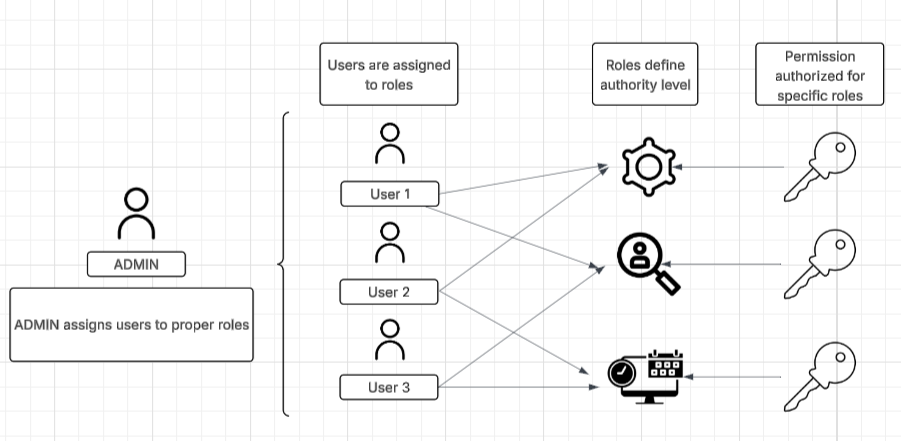
\includegraphics[width=0.75\linewidth]{images/rbac.png}
    \caption{Role-based Access Control}
    \label{fig:rbac}
\end{figure}

This role-driven view fits hospital environments naturally. Hospitals already classify staff by job function and responsibility, such as doctor, nurse, lab technician, or billing staff. When a new staff member joins or changes department, administrators typically think in terms of assigning or removing job functions rather than manually managing hundreds of fine-grained permissions. For this reason, many healthcare systems adopt RBAC as a practical baseline for authorization management \cite{SantosPereira2013, Shin2015}.
\vspace{0.5cm}


To understand RBAC in a concrete way, it helps to follow the typical decision path that a system takes during authorization. After a user is authenticated, the system knows the user identity. RBAC then checks which roles this user has been assigned. Each role represents a set of permissions, where a permission can be understood as an approved operation on a protected resource (for example, \textit{read medical record}, \textit{update lab result}, or \textit{approve discharge}). In daily operation, RBAC often uses the concept of a \textit{session}, where a user activates one or more roles to perform tasks, which supports the principle of least privilege in practice \cite{Sandhu1996, Ferraiolo2007RBAC2E}. In short, RBAC makes authorization decisions by mapping:
\textit{user} $\rightarrow$ \textit{roles} $\rightarrow$ \textit{permissions}.
\vspace{0.5cm}


RBAC also supports more structured control beyond basic role assignment. A common extension is a \textit{role hierarchy}, where senior roles inherit permissions from junior roles. This mirrors real organizational structures (for example, a department head may inherit permissions of a regular physician). RBAC systems can also enforce \textit{constraints}, such as separation of duty, to reduce the risk of misuse and ensure that sensitive workflows cannot be completed by a single user without checks \cite{Sandhu1996, Ferraiolo2007RBAC2E}. These features are particularly relevant in regulated domains like healthcare, where accountability and policy compliance are important \cite{Shin2015}.
\vspace{0.5cm}


However, while RBAC is practical and understandable, hospitals also expose its limitations. Clinical work often depends on \textit{dynamic context}. Access is not decided only by job title. It depends on factors such as whether a doctor is part of the treating team for a particular patient, whether a nurse is on shift and assigned to the same ward, or whether an emergency situation requires controlled override access. A hospital may also classify some records as more sensitive than others, where access rules become stricter \cite{SantosPereira2013}. These conditions change frequently and can be different for the same user across time and location.
\vspace{0.5cm}


When RBAC is used alone, a common response is to create more roles to represent these situations (for example, splitting roles by department, ward, or shift). Over time, this creates an operational burden: the number of roles grows, exceptions accumulate, and policy management becomes harder and more error-prone. In healthcare, this is risky because policy mistakes can either block legitimate care or expose sensitive data \cite{SantosPereira2013, Shin2015}. In addition, emergency access patterns (often described as “break-glass”) show that the system must sometimes allow access outside normal role boundaries while still ensuring strong auditing and justification \cite{SantosPereira2013}. Such requirements are difficult to capture cleanly using roles alone.
\vspace{0.5cm}


For these reasons, RBAC is a strong baseline but not sufficient by itself for fine-grained hospital scenarios. This thesis therefore treats RBAC as the foundation that captures stable organizational responsibilities, and it motivates the need for additional mechanisms that can express context-based conditions in a controlled way. This leads to Attribute-Based Access Control (ABAC) and hybrid RBAC/ABAC approaches, which aim to improve flexibility without losing manageability.


\subsection{Attribute-Based Access Control (ABAC)}
\label{subsec:abac}

RBAC matches the stable structure of a hospital, but many hospital decisions depend on the current situation: which patient is assigned, which ward the staff is working in, whether the staff is on duty, or whether the case is an emergency. ABAC is designed for this kind of problem. Instead of relying mainly on roles, ABAC evaluates an access request by looking at the attributes that describe the request. A common abstraction is that an ABAC decision is driven by the attributes of the subject, the object (resource), the operation (action), and the environment (context) \cite{Zheng2019ABAC}. This makes ABAC naturally suitable for policies like “permit only if the requester is on the care team” or “permit only if ward matches and the request is inside the shift time window.”
\vspace{0.5cm}


To make ABAC usable in real systems, authorization is usually organized into a small set of functional components. Policy Decision Point (PDPs) is component that computes access decisions, and state that one of their primary functions is to \emph{mediate or deconflict} policies  according to metapolicies \cite{NIST800162}. The Policy Enforcement Point (PEP) is responsible for enforcing the PDP decision at the place where the request is made \cite{NIST800162}. The PDP cannot decide without attributes, so it queries a Policy Information Point (PIP), which serves as the retrieval source for the attributes needed for policy evaluation \cite{NIST800162}. In healthcare-oriented ABAC designs, the same idea appears in a practical form: the PDP evaluates policies and attributes, the PEP enforces the permit/deny result, and the PIP provides user, patient, and environment attributes required for correct decisions \cite{Afshar2017ABAC}.

This separation is important for a microservices-based HMS. The PEP can be placed close to each service endpoint (or at an API gateway), while the PDP can be managed centrally as an authorization service. \cite{NIST800162} highlights that PDP and PEP functionality can be centralized or distributed, and that an organization may use a centrally controlled decision service that evaluates attributes and policy and passes decisions back to PEPs \cite{NIST800162}. This is a practical direction for avoiding inconsistent authorization logic across services.


\begin{figure}[H]
    \centering
    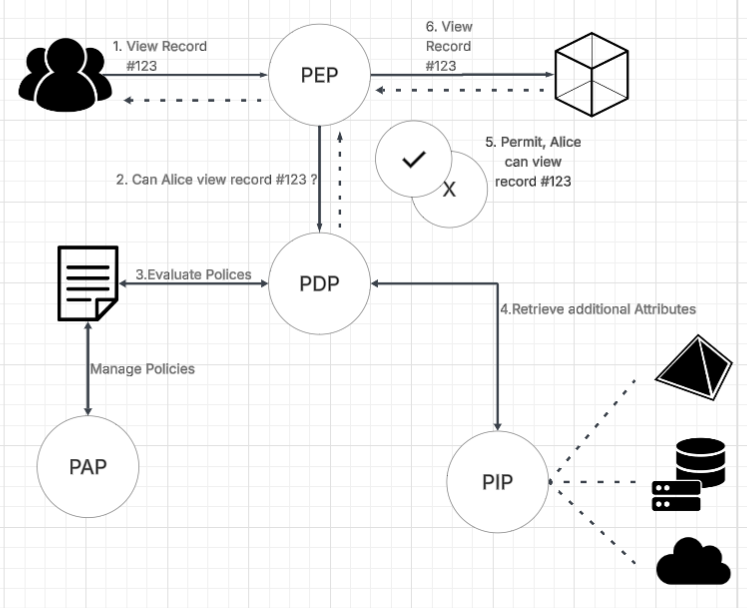
\includegraphics[width=0.75\linewidth]{images/abac.png}
    \caption{The standard architecture for ABAC}
    \label{fig:abac}
\end{figure}
However, ABAC also introduces operational challenges that become visible as policies and systems scale. First, ABAC is only as reliable as its attributes. If attributes such as shift status, ward assignment, care-team relationship, or record sensitivity are missing or outdated, decisions can be wrong even if the policy logic is correct. Second, ABAC tends to grow complex because policies often include many attribute predicates and combinations. \cite{Zheng2019ABAC} points out that ABAC policies become huge and complex in practice, making management difficult and conflicts frequent; they also emphasize that many real security failures come from policy misconfiguration rather than from cryptographic failures \cite{Zheng2019ABAC}. \cite{NIST800162Cost} similarly notes that ABAC is more complicated and therefore more costly to implement and maintain than simpler access control systems \cite{NIST800162Cost}.
\vspace{0.5cm}


One concrete problem that appears in large ABAC deployments is \textbf{policy conflict}. In simple terms, two or more rules may apply to the same request conditions but produce different decisions, which makes the overall behavior hard to predict and difficult to audit. \cite{Shu2009Conflicts} describe this clearly: conflicting rules make different assertions for the same set of user requests, and if conflicts are not detected and resolved, access control can become either too open or too restrictive \cite{Shu2009Conflicts}. Although some policy languages can use rule-combining strategies (e.g., deny-overrides), \cite{Shu2009Conflicts} warn that the result can be unpredictable when the rule set becomes too large to be comprehensible for administrators \cite{Shu2009Conflicts}. Because of this, conflict analysis is often treated as a \emph{pre-deployment} activity: detect conflicts early, fix them before policies are deployed into PDPs.


\subsubsection*{Policy conflict detection}
At a practical level, conflict detection methods aim to do three things:
\begin{enumerate}
    \item \textbf{Identify overlap:} find rules whose conditions can be satisfied by the same request (i.e., they overlap in the attribute space).
    \item \textbf{Check decision disagreement:} among overlapping rules, detect cases where the decision differs (permit vs deny).
    \item \textbf{Output actionable results:} return the pairs (or sets) of conflicting rules, often with supporting information such as which attribute predicates cause the overlap, so that a policy author can fix the policy.
\end{enumerate}

Because ABAC policies can contain many rules and many predicates, the key challenge is efficiency: a naive approach would compare every rule with every other rule and quickly becomes expensive.

\subsubsection*{Method A: Rule reduction + binary search (efficient pre-deployment detection)}
\textbf{Step 1 — Rule reduction (remove redundancy and normalize predicates):}  
The method starts from the observation that large policy sets contain redundancy: multiple rules may share attribute identifiers and overlapping ranges. Rule reduction transforms the original rules into a set of reduced rules whose attribute predicates do not intersect, while keeping the reduced policy \emph{semantically equivalent} to the original one \cite{Shu2009Conflicts}. The benefit is that conflict checking becomes more structured: the reduced rules are compact, and the method avoids repeatedly examining the same predicate patterns across many rules \cite{Shu2009Conflicts}.
\vspace{0.5cm}


\textbf{Step 2 — Binary search (find intersecting predicates efficiently)}  
After reduction, attribute predicates can be sorted, and binary search can be used to quickly identify which predicates intersect with a target predicate. The \cite{Shu2009Conflicts} paper explains that binary search becomes possible because non-intersection is guaranteed by the reduction step, allowing the search space to be halved repeatedly \cite{Shu2009Conflicts}. In implementation, the method also uses bitmap-based set operations for fast intersection/union of candidate rule sets \cite{Shu2009Conflicts}. 
\vspace{0.5cm}


The output is a list of statically-conflicting rules (conflicts detectable without executing real user requests), which can then be reviewed and corrected before deployment \cite{Shu2009Conflicts}. In other words, it supports administrators by turning a large, hard-to-read policy set into a smaller set of clear “conflict candidates”.

\subsubsection*{Method B: Binary sequence encoding + bitwise operations (fast overlap checking)}
This method encodes each ABAC rule into a set of binary sequences and then detects conflicts using bitwise AND operations \cite{Zheng2019ABAC}. The motivation is to improve efficiency when policies are large and complex. The paper explicitly states that the rule is transformed into binary sequences and conflicts are detected via AND operations, which improves detection efficiency \cite{Zheng2019ABAC}.  
\vspace{0.5cm}


Similar to Method A, the practical output is a set of detected conflicts among rules. The key advantage is speed: encoding and bitwise operations provide a computationally efficient way to test overlaps in the attribute space, which becomes useful when the rule set is large \cite{Zheng2019ABAC}.
\vspace{0.5cm}


ABAC provides a strong answer to dynamic hospital constraints because policies can directly reference context and relationships using attributes. At the same time, ABAC introduces new operational risks: attribute governance, policy complexity, and conflicts caused by overlapping rules. Conflict detection methods such as rule reduction + binary search, or binary sequence encoding + bitwise operations, are therefore useful as supporting tools to keep ABAC policies maintainable and safer before deployment \cite{ Zheng2019ABAC}.
\vspace{0.5cm}


These trade-offs lead naturally to hybrid RBAC/ABAC approaches. RBAC offers stability and organizational alignment, while ABAC offers context-sensitive precision. A hybrid model keeps the role structure as the baseline and uses ABAC constraints where hospital workflows require dynamic conditions.


\subsection{Hybrid RBAC/ABAC}
\label{sec:hybrid-rbac-abac}

RBAC and ABAC are often presented as two ends of the same spectrum. RBAC is strong when an organization already has a clear job structure, because administrators can reason in terms of job functions and stable responsibilities. ABAC is strong when access decisions must depend on the current situation, because policies can use subject, object, and environment attributes to express fine-grained rules. In real systems, especially in healthcare, the access control problem usually needs both: a stable role structure \emph{and} frequent context checks. This is the main motivation behind hybrid RBAC/ABAC models: they try to combine the administrative simplicity of RBAC with the expressive power of ABAC, without fully inheriting the weaknesses of either one \cite{KuhnCoyneWeil2010,Penelova2021HRABAC}.
\vspace{0.5cm}


Conceptually, a hybrid RBAC/ABAC decision can be viewed as a conjunction of two checks:

\[
\textit{Permit} \;\Leftrightarrow\; \underbrace{\textit{RBAC}(u,r,p)}_{\text{baseline eligibility}}
\;\wedge\;
\underbrace{\textit{ABAC}(s,o,a,e)}_{\text{contextual constraint}}
\]

where RBAC determines whether the user (or session) has an eligible role and permission, and ABAC evaluates attribute- and context-based conditions (e.g., IP, location, time, sensi tivity) before the permission is actually exercised. Depending on how roles and attributes are combined, the literature commonly distinguishes the following hybrid variants.
\vspace{0.5cm}


A hybrid model is not a single fixed architecture. It is a family of designs that connect roles and attributes in different ways. A useful way to think about hybridization is to ask: \emph{Where do roles end and where do attributes begin in the decision?} Some systems use attributes mainly to \emph{choose} roles, while others keep roles as the main structure and use attributes mainly to \emph{constrain} permissions. \cite{KuhnCoyneWeil2010} describes common RBAC-with-attributes directions (often called RBAC-A) and show that hybridization can reduce policy complexity compared to encoding everything as roles or everything as attribute rules \cite{KuhnCoyneWeil2010}. In other words, hybrid models are mostly about \emph{splitting the decision problem} so that each part is handled by the mechanism that fits it best. Across existing work, three practical hybrid patterns appear frequently.
\vspace{0.5cm}


First, \textbf{attribute-driven role activation (dynamic roles)} uses attributes to decide which roles are active for a user in a given session. The system keeps a role structure, but the role activation becomes context-dependent. This can reduce manual role switching and can be suitable when a small number of context variables controls access (e.g., on-site vs off-site). However, if the environment is rich in attributes, dynamic-role designs can quickly become hard to manage because many role activation combinations need to be considered \cite{KuhnCoyneWeil2010}.
\vspace{0.5cm}

\begin{figure} [H] 
    \centering
    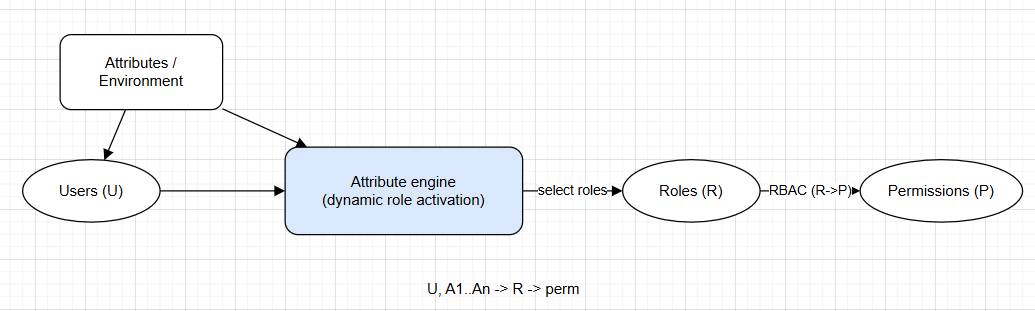
\includegraphics[width=0.75\linewidth]{images/dynamics-role.png}
    \caption{Attribute-driven role activation (dynamic roles) \cite{KuhnCoyneWeil2010}}
    \label{fig:dynamics-role}
\end{figure}

Second, \textbf{role-as-an-attribute (attribute-centric hybrids)} treats the role itself as one attribute among others. The access decision is computed by an ABAC-style policy engine, but one of the key attributes is the user’s job function or organizational position. This approach is conceptually simple because there is one evaluation mechanism (ABAC). The trade-off is that the policy layer can grow large, and the system may lose some of the practical benefits of RBAC administration (such as role hierarchy reasoning and simple permission reviews) unless the policy tooling is strong \cite{KuhnCoyneWeil2010}.
\begin{figure}[H]
    \centering
    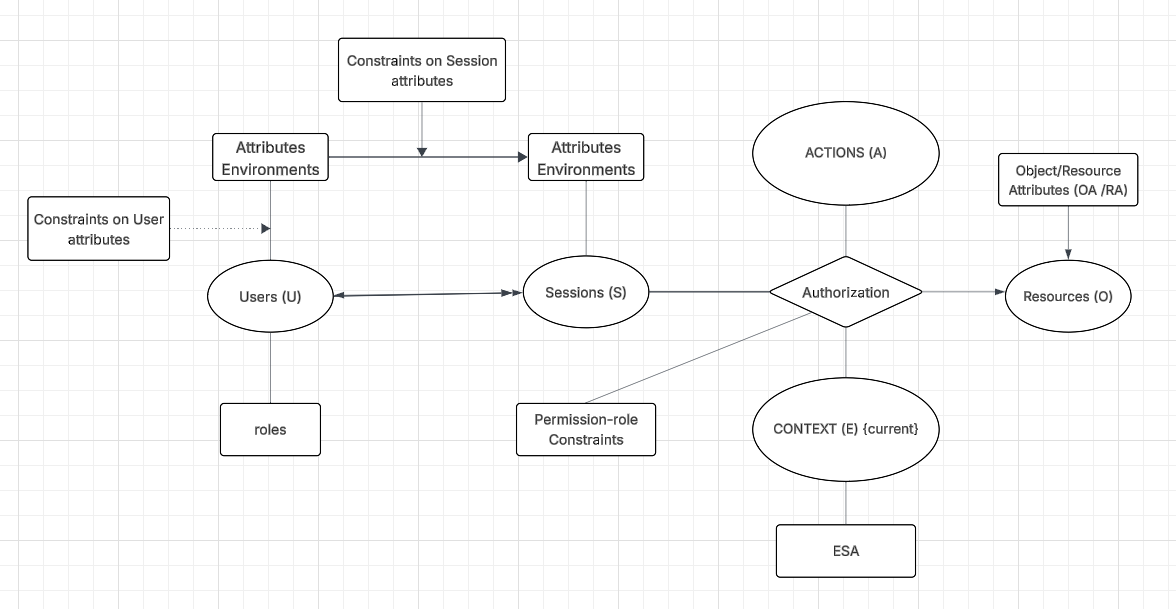
\includegraphics[width=0.75\linewidth]{images/attribute-centric.png}
    \caption{Attribute-centric (ABAC-first) hybrid model \cite{KuhnCoyneWeil2010}}
    \label{fig:placeholder}
\end{figure}


Third, \textbf{role-first with attribute constraints (role-centric hybrids)} starts from RBAC permissions but refines the decision using attributes. In this pattern, roles define the baseline permission set, and attributes act as constraints (for example, patient relationship, shift, location, data sensitivity, or emergency state). The key benefit is that organizations keep the familiar role hierarchy as the “main map” of responsibilities, while still enforcing fine-grained rules where needed \cite{KuhnCoyneWeil2010}. Many practical “RBAC + extra checks” implementations fall into this category; for example, Penelova proposes HRABAC as an extension of RBAC that adds attribute-based policy functions to protect data even when a role-level action is granted \cite{Penelova2021HRABAC}.
\begin{figure}[H]
    \centering
    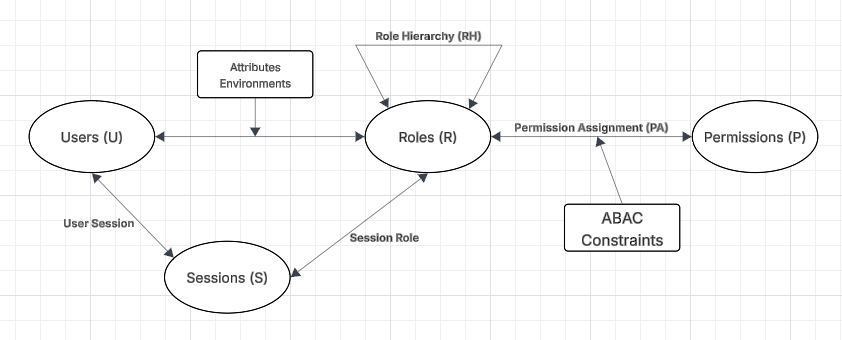
\includegraphics[width=0.75\linewidth]{images/role-centric.png}
    \caption{Role-centric (RBAC-first) hybrid model \cite{Houhou2024HyARBAC}}
    \label{fig:placeholder}
\end{figure}
Beyond RBAC-A, there are also \textbf{composite or layered designs} that explicitly combine multiple engines. One common form is a two-step decision: an RBAC step checks whether the action is allowed in principle for the user’s role, and an ABAC step then checks additional constraints. A cloud-oriented example is HyARBAC, which combines RBAC and ABAC so that access is not granted purely by role membership but also depends on attribute checks, aiming to improve flexibility while keeping RBAC’s administrative structure \cite{Houhou2024HyARBAC}. Layered hybrids are appealing in distributed systems because they naturally support separation of concerns: role administration can remain stable, while attribute policies evolve as business and compliance requirements change.
\vspace{0.5cm}


Hybridization does not automatically remove RBAC and ABAC problems; instead, it allows the system to apply \emph{targeted} solutions from each side.
\vspace{0.5cm}


From the RBAC side, role engineering (defining roles, hierarchies, and constraints) remains important because roles are still the main organizational structure in most hybrids. Role hierarchies and separation-of-duty constraints keep the baseline permissions consistent and reviewable. In a hybrid design, this baseline acts as the first control layer: it limits the maximum set of actions a user can attempt, which reduces the number of attribute rules that need to be evaluated for every request \cite{KuhnCoyneWeil2010}.
\vspace{0.5cm}


From the ABAC side, governance of attributes (where attributes come from, how they are validated, and how policies are maintained) becomes the main quality factor. Importantly, the policy-conflict detection techniques discussed in Section~2.2.2 become directly useful in hybrids as well. Even if RBAC defines the baseline permissions, the ABAC constraints still need to be correct and consistent. In practice, conflict detection in a hybrid model should do two things: (1) detect conflicts inside the attribute policy set itself (e.g., contradictory rules for the same request context), and (2) detect mismatches between role permissions and attribute constraints (e.g., a role grants an action broadly, but attribute rules deny it in almost all contexts, which may indicate a design error or a missing role refinement). Because the ABAC part is usually the more complex and more frequently updated part, applying conflict detection and policy validation there helps keep the entire hybrid model stable over time \cite{Houhou2024HyARBAC}.
\vspace{0.5cm}


This thesis targets an HMS deployed as a microservices-based application, where authorization must be both strict and operationally practical. In a hospital, job functions and reporting structure are stable and well understood (e.g., doctor, nurse, lab technician, pharmacist, receptionist). At the same time, real access needs are highly context-dependent: ward assignment, care-team relationship, shift schedule, emergency state, and data sensitivity can change frequently. For this reason, a hybrid model is a natural fit: it allows the system to keep a clear role baseline while enforcing the dynamic checks that appear in everyday clinical workflows.
\vspace{0.5cm}


Based on the hybrid patterns above, the implementation in this thesis will adopt a \emph{role-first hybrid approach} for the HMS, but only as the final design choice after reviewing the broader hybrid space. Concretely, roles will define the baseline permissions and the organizational hierarchy, while ABAC constraints will refine access for sensitive operations and patient-specific data access. This direction matches the hospital’s natural structure and supports clear auditing: administrators can still explain \emph{who is allowed to do what} at the role level, while the attribute layer explains \emph{under which conditions} the action is allowed. This choice also aligns with practical hybrid designs that extend RBAC with additional attribute-based checks to protect sensitive records \cite{KuhnCoyneWeil2010,Penelova2021HRABAC}.




\section{Microservices}
\label{sec:microservices}

\subsection{Definition of Microservices}
\label{sec:microservices-definition}
Microservices are commonly understood as an architectural style where an application is built as a set of small services that run independently and cooperate through lightweight communication. Each service is designed around a clear business capability, so teams can develop, test, and deploy services without having to ship the whole system at the same time. This is one of the main reasons microservices are often chosen for large domains like hospital management systems, where the system naturally splits into areas such as patient records, appointments, laboratory workflows, billing, and reporting.
\vspace{0.5cm}

In practice, microservices are less about “splitting code into many repositories” and more about setting boundaries that reduce tight coupling. A useful rule is that a service should hide its internal implementation details and expose only what other services need through an interface. This supports independent evolution: when one service changes internally, other services do not need to change as long as the interface remains compatible. Microservices are also typically associated with automation and fast release cycles, because small services are easier to build and deploy repeatedly than a large monolith \cite{BaresiGarriga2020,AbdelfattahCerny2022}.

\subsection{Design Principles of Microservices Architecture}
\label{sec:microservices-principles}
When building an application using microservices, the first practical step is choosing service boundaries. A common approach is to align services with business capabilities and keep each service scope “bounded”, meaning it owns a coherent part of the domain. This reduces cross-service dependencies and makes it realistic for teams to work in parallel. Once boundaries are defined, the architecture should aim for “share as little as possible” between services. Shared databases or shared internal libraries may look convenient at first, but they often recreate the same tight coupling that microservices are meant to avoid \cite{BaresiGarriga2020}.
\vspace{0.5cm}

The second step is defining how services communicate. In most microservice systems, service-to-service calls are implemented using lightweight mechanisms (for example REST APIs or messaging), with clear contracts. This contract-first mindset matters because it forces the system to be explicit about what data is exchanged and why. It also makes it easier to introduce versioning and gradual rollout strategies when interfaces evolve. In other words, microservices work well when services can tolerate change around them without breaking \cite{BaresiGarriga2020}.
\vspace{0.5cm}

The third step is enabling independent deployment through automation. Microservices are expected to be independently deployable, so the engineering workflow usually includes CI/CD pipelines, container-based packaging, and operational monitoring. The point is not the specific tool, but the capability: each service should be buildable, testable, and deployable on its own. This also implies that failures must be handled as normal conditions in distributed systems. Typical practices include health checks, timeouts, and resilience patterns to avoid one failing service causing a full-system outage \cite{AbdelfattahCerny2022,Yarygina2018}.
\vspace{0.5cm}

Finally, microservices require operational visibility. Because requests often pass through multiple services, teams need logging and monitoring that can follow a request across service boundaries. Without this, troubleshooting becomes difficult and security incidents become harder to investigate. As a result, observability is not an optional “nice-to-have” in microservices; it is part of what makes the architecture manageable \cite{AbdelfattahCerny2022}.

\subsection{Direct Connection to Hybrid Access Control}
\label{sec:microservices-hybrid-connection}
Microservices change the access control problem in a very direct way: instead of one application making one decision, there are many services making decisions across a request chain. If each microservice implements authorization rules in its own way, the system can quickly accumulate duplication and inconsistency. Prior work highlights a recognized need to apply security control policies consistently across microservices in the same system \cite{AbdelfattahCerny2022}.
\vspace{0.5cm}


A common architectural response is to use an API gateway as a controlled entry point. The gateway can act as a proxy and policy enforcement point that separates external clients from internal services, and it often takes responsibility for request routing and authentication at the edge \cite{AbdelfattahCerny2022}. However, edge checks alone are not sufficient for healthcare scenarios, because fine-grained authorization frequently depends on internal context (e.g., care-team relationship, ward assignment, emergency status). Therefore, authorization must remain enforceable at the service level as well.
\vspace{0.5cm}


This is where the connection to Hybrid RBAC/ABAC becomes natural. RBAC provides a stable baseline that matches hospital structure (roles such as doctor, nurse, lab technician), while ABAC provides the dynamic conditions that appear in real workflows (shift, location, patient consent, emergency override). In microservices, those decisions must also be consistent along the full request path. Research emphasizes that distributed components require propagating the user’s authentication and authorization identity throughout the full communication cycle, commonly using token-based mechanisms such as JWT \cite{AbdelfattahCerny2022,Yarygina2018}. This aligns well with a hybrid design where role information can be carried as a base claim, while required attributes can be fetched or evaluated when a service makes a decision.
\vspace{0.5cm}


In this thesis, these microservice properties motivate implementing authorization as a reusable capability rather than scattered logic: an authorization decision function (PDP-like) can be shared as a service, while each microservice acts as a local enforcement point (PEP-like) at the time it performs a sensitive operation. This structure supports consistent decisions, reduces duplicated rules, and keeps the access model aligned with the hospital’s role hierarchy while still handling dynamic clinical context \cite{AbdelfattahCerny2022}.





\chapter{System Analysis \& Design}
\section{System Design Overview}

\subsection{Scope and design goals}
This thesis designs and demonstrates a hospital management system (HMS) using a microservices architecture, with a focus on enforcing access control through a role-centric hybrid RBAC/ABAC model (RBAC-A) as presented in \cite{KuhnCoyneWeil2010}. The goal is to show how fine-grained authorization can be applied in a realistic hospital setting without making the system difficult to maintain.
\vspace{0.5cm}


To keep implementation and evaluation manageable for a bachelor thesis, the prototype scope is intentionally limited to seven core services that represent the most common clinical and administrative workflows. These services include the User Service for staff profiles and role bindings, the Patient Service for patient information and medical records, the Appointment Service for scheduling, the Lab Service for lab orders and results, the Pharmacy Service for prescriptions and dispensing, the Billing Service for invoices and payments, and the Audit Service for access logs. Each service follows independent data ownership (database per service). Supporting services that can exist in a full HMS (such as notifications or reporting) are not included because they are not required to demonstrate and evaluate the hybrid authorization model.
\vspace{0.5cm}


Even with this limited scope, the system still covers the main situations where access control matters most: viewing patient records, booking appointments, issuing and dispensing prescriptions, and handling billing. These workflows also differ in resource types and sensitivity, which makes them suitable for demonstrating policies that depend on both roles and context. At the same time, keeping the scope small helps keep the policy set understandable and testable.

\subsection{Actors}
\label{subsec:actors}
The prototype is built around common hospital roles and their daily tasks. Doctors access patient records, document clinical information, order lab tests, and issue prescriptions. Nurses support patient care and update information based on assigned duties. Receptionists handle appointment booking and basic administrative updates, typically without access to detailed medical content. Lab technicians create or update test status and publish lab results, mostly within the Lab Service. Pharmacists verify prescriptions and dispense medicine, with operations centered around prescription state and inventory updates. Billing clerks create invoices and record payments, and administrators manage users, roles, and authorization policies. The system also includes a patient role, which is usually restricted to viewing only personal information such as one’s own appointments and payment status.
\vspace{0.5cm}


These actors reflect a typical RBAC structure used in hospitals, but many real decisions still depend on attributes such as department, assignment, and time conditions. This is the motivation for combining RBAC with ABAC constraints in a controlled way.

\subsection{System Overview diagram}
Figure~\ref{fig:systemoverview} summarizes the overall system design using a layered view. The architecture separates client access, edge enforcement, authorization decision-making, and business microservices.


\subsubsection{Layer A — Client/UI:} Users interact with the system through the portal or mobile app. Authentication is handled by an Identity Provider that issues access tokens (JWT).

\subsubsection{Layer B — Edge:} The API Gateway/BFF acts as the primary Policy Enforcement Point (PEP). It intercepts incoming requests, validates the token, and requests an authorization decision before routing the request to a target service.

\subsubsection{Layer C — Authorization:} A centralized Authorization Service acts as the Policy Decision Point (PDP). It evaluates access requests using role-centric Hybrid RBAC/ABAC rules. Policy definitions and constraints are managed in a policy store, and required attributes/context can be provided via an attribute provider.

\subsubsection{Layer D — Business Services:} Domain microservices implement HMS business functions such as Patient record, scheduling, lab results, billing, pharmacy, etc. Each service owns its data store.

A typical request follows these steps:
\begin{itemize}
    \item The user logs in and receives a JWT from the Identity Provider.
    \item The client sends an HTTPS request with the JWT to the API Gateway/BFF.
    \item The Gateway sends an authorization decision request to the Authorization Service.
    \item The Authorization Service returns a Permit or Deny decision.
    \item If permitted, the Gateway routes the request to the target microservice.
\end{itemize}

\begin{figure}[H]
    \centering
    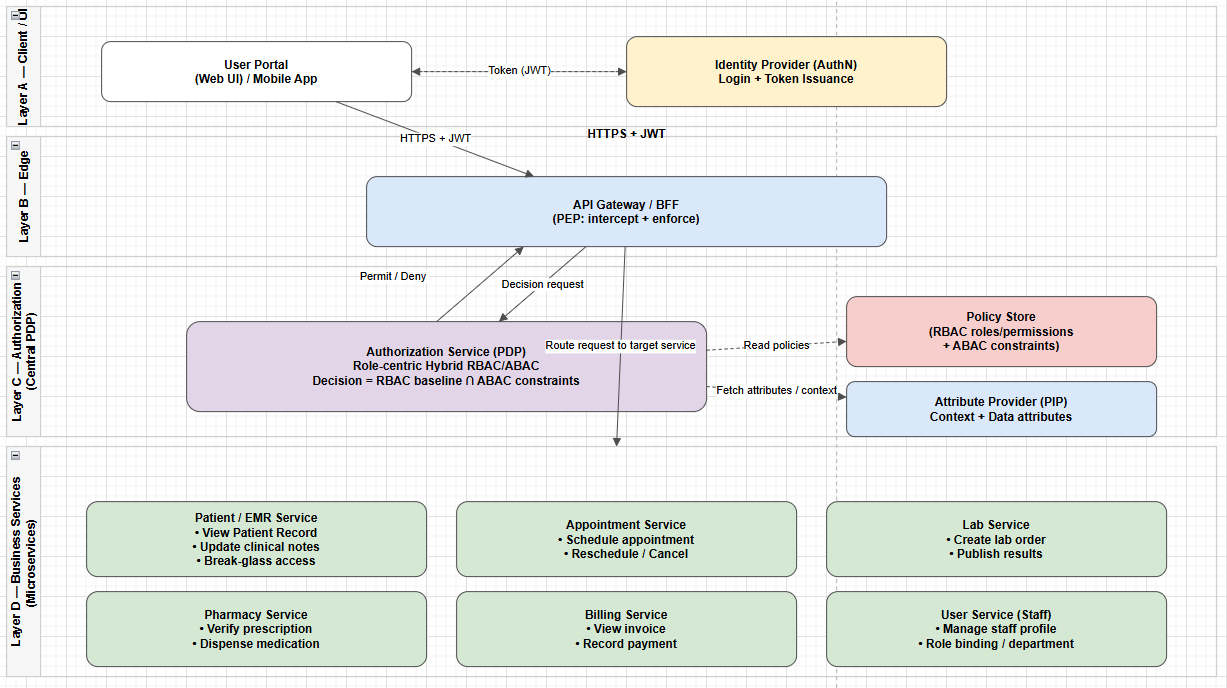
\includegraphics[width=1\linewidth]{images/systemoverview.png}
    \caption{System Overview Diagram}
    \label{fig:systemoverview}
\end{figure}
\section{System Architecture}
This section describes how the HMS prototype is structured and how requests move through the system. The design follows a microservices approach and uses a centralized authorization service (central PDP) to make access decisions consistently across services.

\subsection{Microservices decomposition}
The prototype is divided into seven business services with clear boundaries. The User Service stores staff profiles and organizational information that is relevant for authorization, such as department and job position. The Patient Service manages patient information and medical record data. The Appointment Service handles scheduling and appointment lifecycle. The Lab Service manages lab orders and results. The Pharmacy Service manages prescriptions and medication dispensing actions. The Billing Service handles invoices and payment records. Finally, the Audit Service records access decisions and request metadata to support traceability and compliance.
\vspace{0.5cm}


This decomposition is useful not only for modular development, but also for authorization clarity. Instead of treating the system as one large application, access can be controlled by resource type such as patient records, lab results, prescriptions, and invoices. This aligns well with hospital workflows and helps policies remain readable.


\subsection{Data ownership}
The application applies the database-per-service principle. Each microservice owns its database, and other services do not read it directly. Data sharing, when necessary, happens through APIs. This matters in a hospital setting because data is sensitive and should not be implicitly exposed through direct database access patterns.
\vspace{0.5cm}


At the same time, authorization decisions often require context from multiple sources. For example, a decision might depend on a staff member’s department (from the User Service) and a resource attribute such as the patient’s ward or record sensitivity (from the Patient Service). Instead of breaking data ownership by letting services query each other’s databases, this thesis uses an attribute provider pattern (PIP). The PIP retrieves only the minimal attributes needed for a decision by calling service APIs, which preserves isolation and reduces unintended data exposure.


\subsection{System Architecture Diagram}
\label{sec:sysarchitecture}
Figure~\ref{fig:archdiagram} illustrates the full architecture used in this thesis. The key idea is that enforcement happens at the edge, while decisions are evaluated centrally. This also defines a clear trust boundary: the client is not trusted to enforce access rules, so all requests must pass through the gateway.
\vspace{0.5cm}


The API Gateway/BFF is the main entry point for client requests and serves as the PEP. It validates JWT tokens, extracts basic identity claims, constructs an authorization decision request, calls the PDP, and forwards the request only when the result is Permit. Authentication is handled by an OIDC/OAuth2 Identity Provider, which manages users and roles and issues JWT tokens.
\vspace{0.5cm}


The Authorization Service is the PDP. It evaluates the role-centric hybrid model used in this thesis: RBAC provides the baseline role-to-permission mapping, and ABAC introduces constraints based on context and resource attributes. Policies are managed separately through a Policy Service (PAP) and stored in a dedicated policy database. The policy store acts as the source of truth, while OPA holds a deployed copy used for evaluation. When additional attributes are required, the PDP calls the PIP to fetch them from relevant domain services. Finally, the system records decision logs in the Audit Service to support traceability.

\subsubsection{API Gateway / BFF (PEP)}
The gateway is the entry point for client requests. It acts as the main enforcement point (PEP). Its job is:
\begin{itemize}
    \item receive HTTPS requests from clients,
    \item validate the access token (JWT),
    \item build an authorization request (who, what action, what resource, and basic context),
    \item ask the Authorization Service for a decision,
    \item only route the request to the target service if the decision is Permit.
\end{itemize}

\subsubsection{Identity Provider (Authentication)}
Authentication is handled by an identity provider (OIDC/OAuth2). Users log in and receive a JWT. The gateway uses this token to identify the user and extract basic claims.
\subsubsection{Authorization Service (PDP)}
This service is the decision point (PDP). It evaluates the hybrid model used in this thesis:
\begin{itemize}
    \item RBAC provides the baseline (role → permissions),
    \item ABAC adds constraints (context and data attributes).
\end{itemize}

The PDP returns \textbf{Permit/Deny}, and it may include simple obligations (e.g., logging requirements). The detailed policy logic is described later in Section 3.4.

\subsubsection{Policy Service (PAP) and Policy Store}
Policies are managed separately from business services. A policy admin updates policies through the PAP. Policies are stored in a dedicated policy store managed by the Policy Service, and the deployed policy set is published to OPA for evaluation by the PDP. This separates policy management from the application logic and keeps changes controlled.

\subsubsection{Attribute Provider (PIP)}
Some access decisions need extra data that is not in the JWT. For example: staff department, patient care-team relationship, and appointment assignment. The PIP fetches these attributes from the relevant services (User/Patient/Appointment). The PDP uses these attributes to evaluate ABAC constraints.
\subsubsection{Audit Service}
The system writes decision logs to an audit log store. This supports traceability, which is important in hospital systems. In this implementation, the audit flow is kept simple: it records the authorization decision and a small set of request metadata.
\begin{figure}[H]
    \centering
    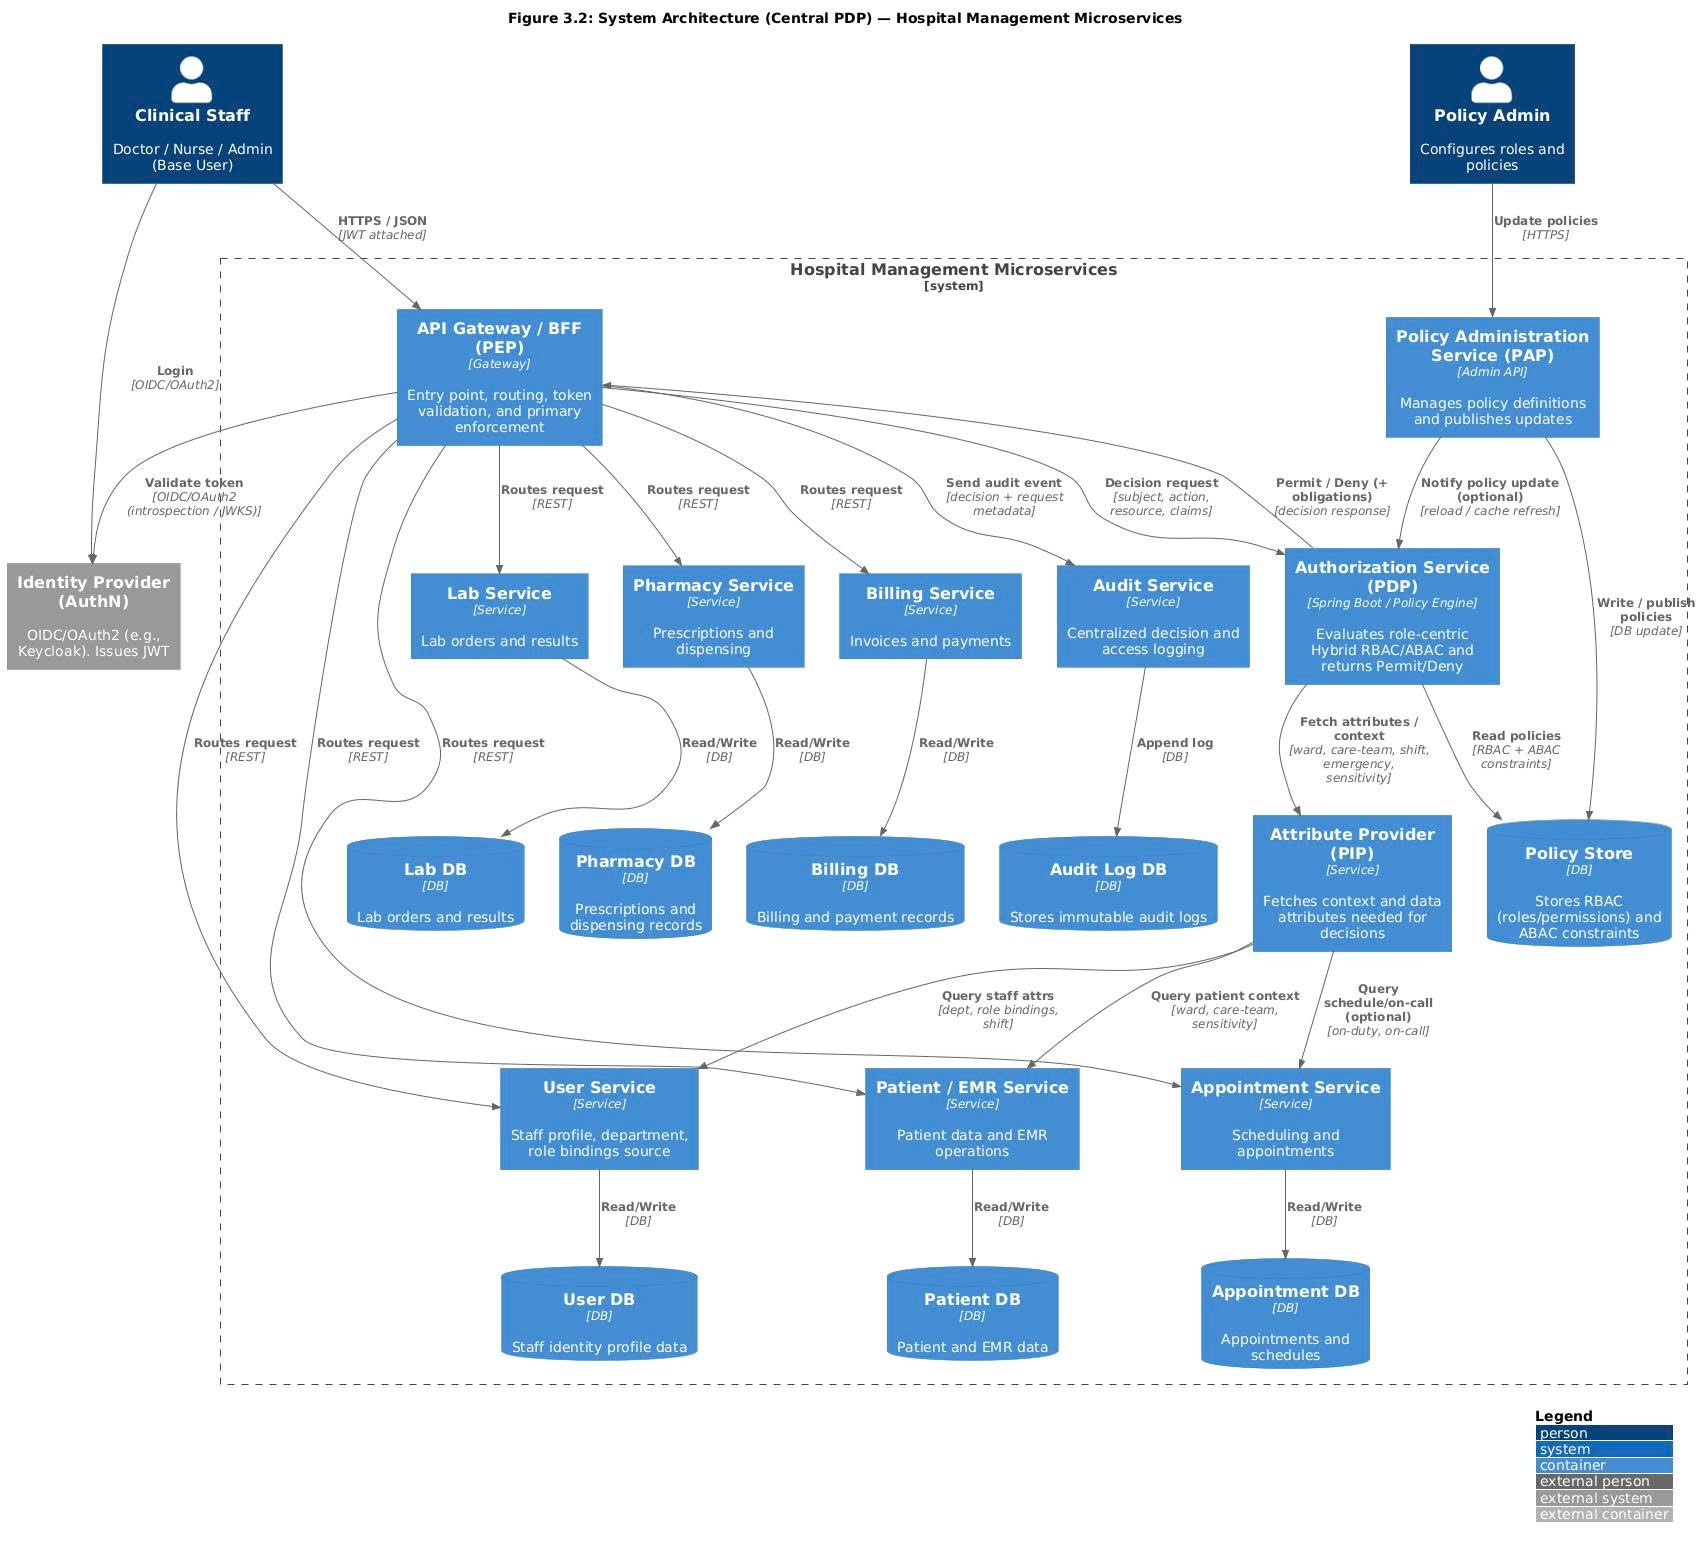
\includegraphics[width=1\linewidth]{images/architecturediagram.png}
    \caption{Architecture Diagram - Hospital Management Microservices}
    \label{fig:archdiagram}
\end{figure}
Figure~\ref{fig:archdiagram} also shows the trust boundary in the system. The client is not trusted to enforce access rules, so all requests must go through the gateway. Business services focus on domain logic and do not decide authorization on their own in this prototype. This keeps the behavior consistent: the same role and context should lead to the same Permit/Deny decision no matter which service is called.
\subsection{Authorization flow}
Figure~\ref{fig:seqdiagram} presents the request flow for a common HMS scenario: a doctor views a patient record. In this flow, the user has already logged in through the Identity Provider, so the client sends an HTTPS request with a valid JWT in the \texttt{Authorization: Bearer <JWT>} header. The gateway first validates the token and extracts basic claims such as user id and role. If the token is missing, expired, or invalid, the gateway stops the request early and returns \texttt{401 Unauthorized}.


\begin{figure}[H]
    \centering
    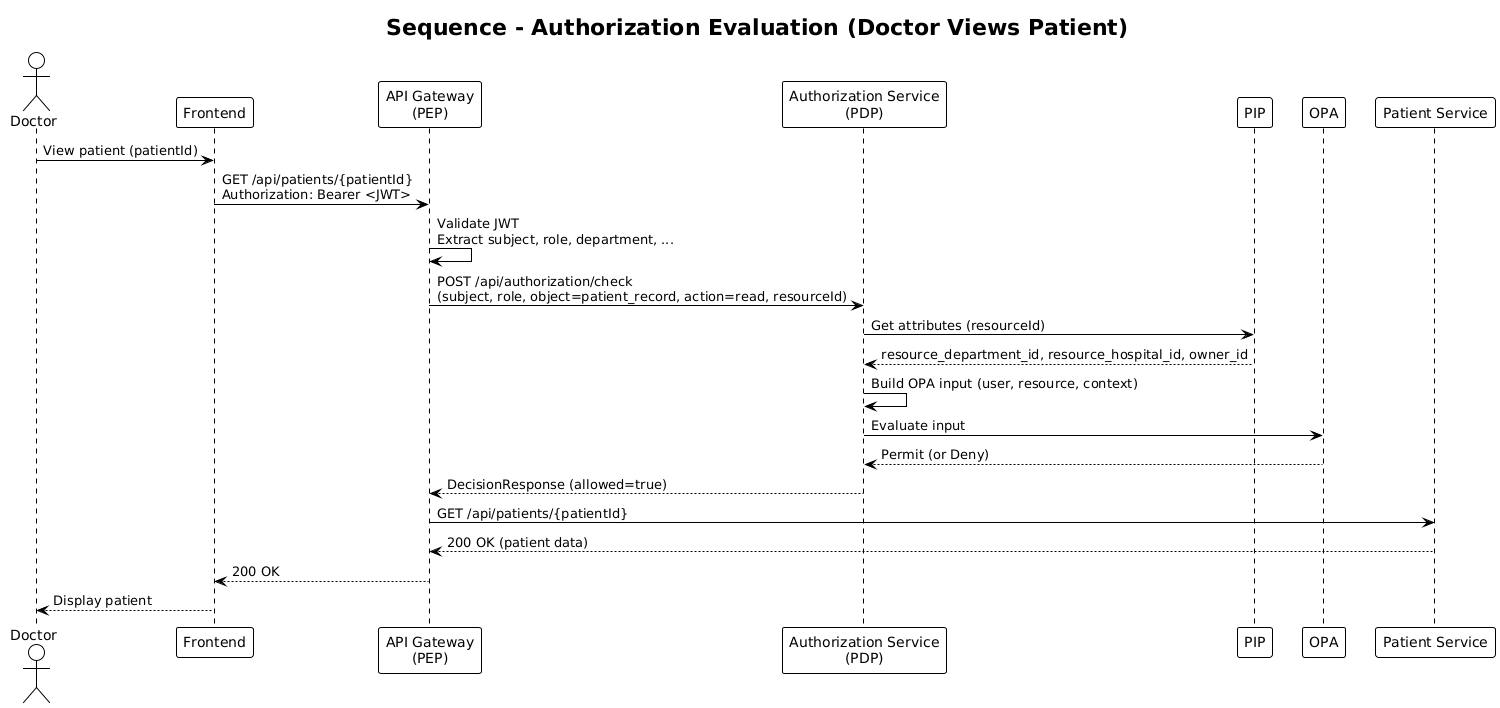
\includegraphics[width=1\linewidth]{images/sequencediagram.png}
    \caption{Sequence Diagram - Doctor View Patient}
    \label{fig:seqdiagram}
\end{figure}
When authentication succeeds, the gateway builds a decision request and sends it to the Authorization Service. The decision request captures the core information needed for authorization, including the subject, the requested action (such as \texttt{read} or \texttt{update}), the resource type and identifier (for example, \texttt{patient\_record} and \texttt{patientId}), and basic request context.
\vspace{0.5cm}


Next, the PDP requests additional attributes through the PIP when necessary. This is important because many hospital decisions cannot rely on JWT claims alone. For example, determining whether a doctor can access a specific patient record may require department matching, assignment information, or resource sensitivity flags. In this design, the PIP returns only the attributes required to evaluate constraints, not full domain payloads such as the complete medical record. This keeps authorization efficient and reduces the risk of exposing sensitive data during decision-making.
\vspace{0.5cm}


After collecting the needed attributes, the PDP builds the final policy input and evaluates it using the policy engine (OPA). OPA returns a Permit or Deny decision, optionally with small metadata for logging and debugging. The gateway then enforces the result: it forwards the original request only when access is permitted, and otherwise returns a forbidden response without calling the business service. The same pattern applies to other protected actions such as dispensing medication or creating an invoice. What changes across workflows is mainly which attributes are required for ABAC constraints.

\section{Key Workflows and Use Cases}
This section highlights representative workflows that are used later for implementation and evaluation. The intention is to show where RBAC is sufficient, where it becomes too rigid, and how the hybrid RBAC-A design helps by adding constraints in a controlled way. Diagrams provide a quick view of the flow, while short descriptions clarify how authorization is applied before state-changing operations reach domain services.


\subsection{Authorization and policy management}
\label{subsec:workflow_auth_policy}
Figure~\ref{fig:activityauthorization} illustrates how a protected request is evaluated by the system. The design separates enforcement from decision-making. The gateway enforces the outcome by allowing or blocking traffic, while the PDP evaluates policy logic and constraints. This separation keeps business services unchanged and avoids duplicating authorization checks inside every microservice.

\begin{figure}[H]
    \centering
    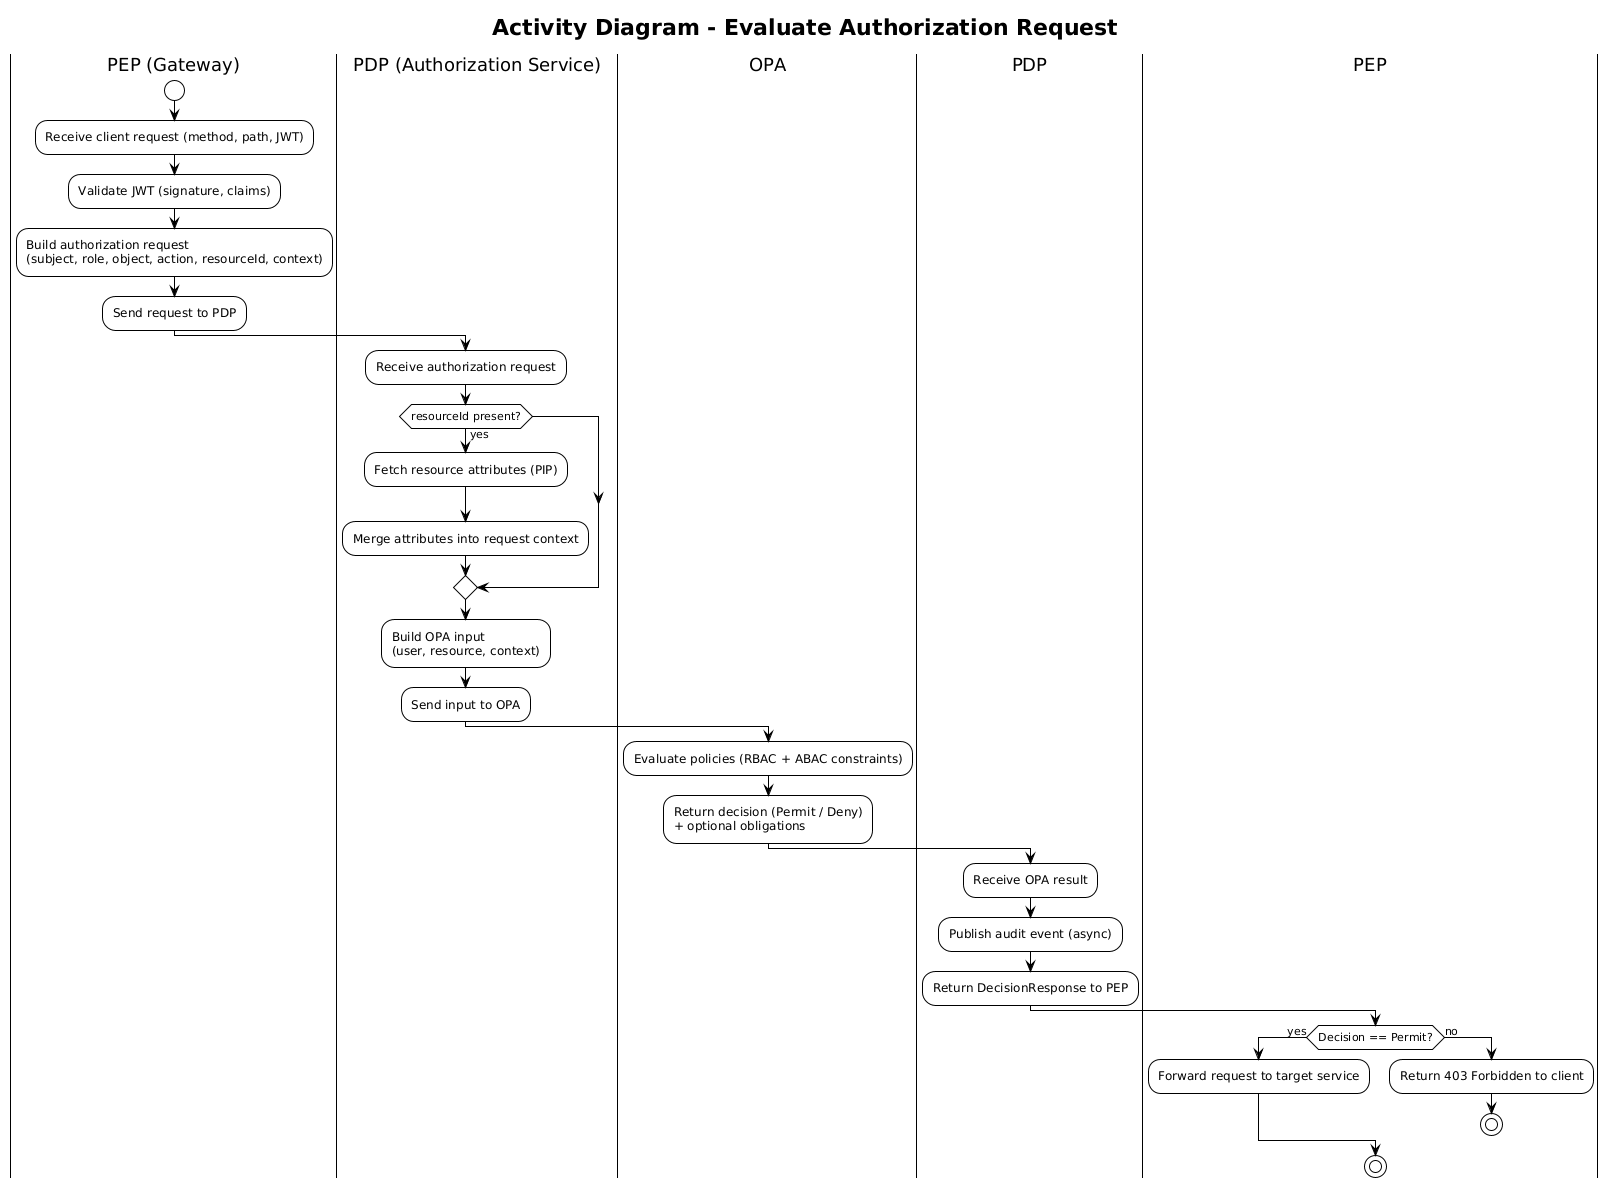
\includegraphics[width=1\linewidth]{images/activityauthorization.png}
    \caption{Activity Diagram - Evaluate Authorization Request}
    \label{fig:activityauthorization}
\end{figure}
In practice, the gateway translates an HTTP request into a decision request that contains the subject, action, resource, and basic context. The PDP enriches the request with missing attributes through the PIP when needed and evaluates constraints using OPA. If the final result is Deny, the request is stopped at the gateway and never reaches the target service. This is important because it reduces the chance of partial information leakage, such as revealing service behavior through timing differences or detailed error responses.
\subsection{Appointment Management}
\subsubsection{Use case diagram}
Booking an appointment is a workflow where RBAC alone is often not enough. Multiple roles may create an appointment, such as patients and receptionists, but the action should still be constrained by hospital scope, department, and other context. Figure~\ref{fig:usecaseappointment} shows the use case view for appointment booking. In this thesis, the action is modeled as \texttt{appointment:create} and the resource type is \texttt{appointment}. The authorization check is performed before the Appointment Service proceeds with slot availability checks and appointment creation.

\begin{figure}[H]
    \centering
    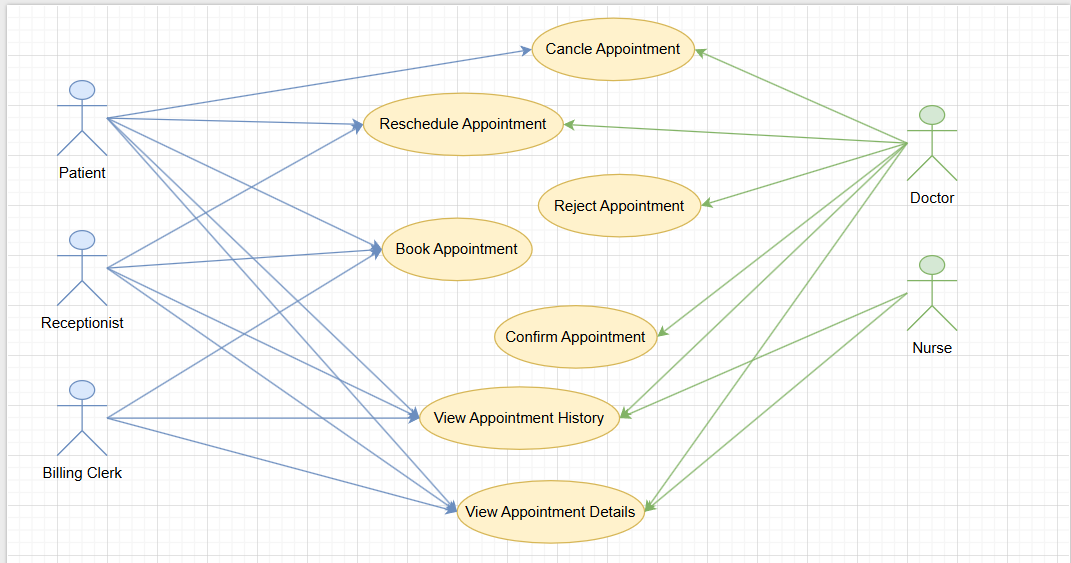
\includegraphics[width=1\linewidth]{images/use-case-appointment.png}
    \caption{Use Case Diagram - Booking Appointment}
    \label{fig:usecaseappointment}
\end{figure}


\subsubsection{Use case table}
\begin{table}[H]
\centering
\label{tab:uc-appointment}
\begin{tabular}{|l|p{9cm}|}
\hline
\textbf{Name} & \textbf{Description} \\
\hline
Actor & Patient, Receptionist, Billing Clerk, Doctor, Nurse \\
\hline
Main function & Book Appointment \\
\hline
Brief description & The Receptionist (or Patient) selects a patient and a preferred time slot, then submits a booking request. The system checks the user's authorization (role and context) and the availability of the slot. If permitted and the slot is available, a new appointment is created with status PENDING\_CONFIRMATION. The Doctor may later Confirm or Reject the appointment. \\
\hline
Context information & User is logged in; appointment management module is available. Patient and doctor/department are known. \\
\hline
\end{tabular}

\end{table}




\begin{table}[H]
\centering
\begin{tabular}{|l|p{9cm}|}
\hline
\textbf{Name} & \textbf{Description} \\
\hline
Triggers & User must be authenticated (JWT). User must have permission to create appointments (e.g. Receptionist, Billing Clerk, or Patient role). At least one time slot must be selectable. \\
\hline
Flow of events summary & 
1. Receptionist or Patient opens the appointment booking page. \\
& 2. User selects patient (if Receptionist/Billing Clerk) and preferred date/time slot. \\
& 3. User submits the booking request. \\
& 4. System (PEP) validates JWT and sends an authorization request to the PDP. \\
& 5. PDP evaluates RBAC and ABAC; if Deny, system returns \texttt{403 Forbidden}. \\
& 6. System checks slot availability in the Appointment Service. \\
& 7. If the slot is available, system creates the appointment and returns confirmation. \\
& 8. Doctor may later confirm or reject the appointment. \\
\hline
\end{tabular}
\caption{Use case table: Book Appointment (Appointment Management)}
\label{tab:uc-appointment}
\end{table}
\vspace{1em}







\subsubsection{Activity Diagram}
\begin{figure}[H]
    \centering
    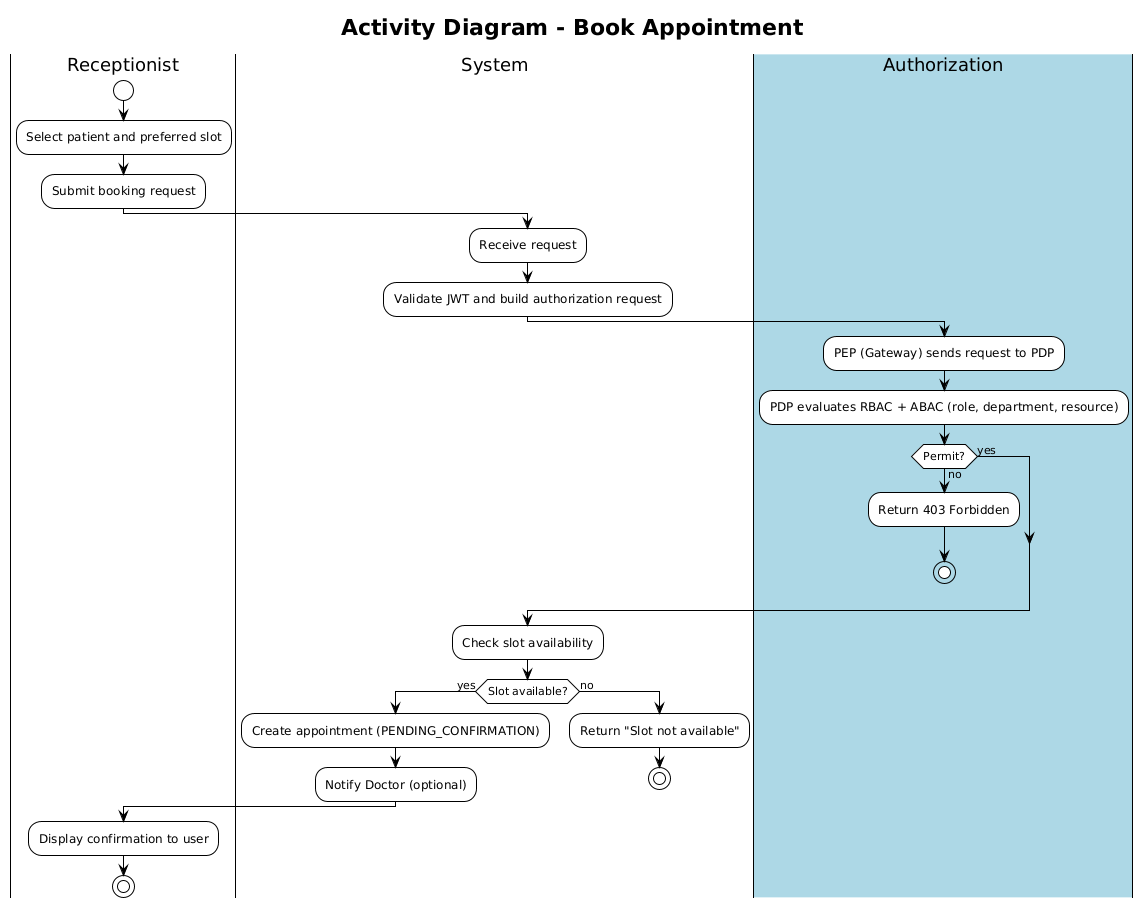
\includegraphics[width=0.75\linewidth]{images/activity-appointment.png}
    \caption{Activity Diagram - Booking Appointment - Receptionist}
    \label{fig:activityappointment}
\end{figure}



\subsubsection{Sequence Diagram}
\begin{figure}[H]
    \centering
    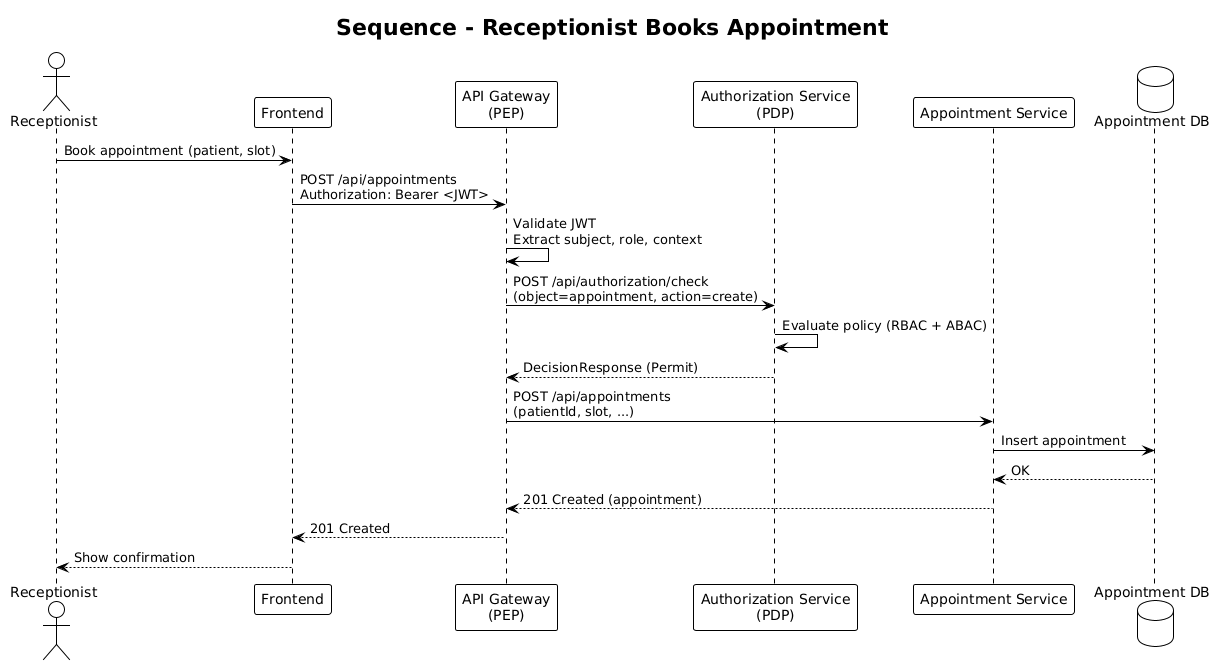
\includegraphics[width=1\linewidth]{images/sequence-appointment.png}
    \caption{Sequence Diagram - Booking Appointment - Receptionist}
    \label{fig:seqappointment}
\end{figure}
In this workflow, the receptionist selects a patient and a preferred time slot, then submits a booking request through the UI. The request goes to the gateway, which validates the JWT and asks the PDP for a decision. If the decision is Deny, the system stops early. If it is Permit, the Appointment Service continues by checking whether the slot is available and then creates a new appointment with status \texttt{PENDING\_CONFIRMATION}. A doctor can later confirm or reject the appointment, which introduces a second set of actions with different authorization requirements.


\subsection{Prescription \& Pharmacy }
Dispensing medication is sensitive because it changes prescription state and inventory records. RBAC provides the baseline permission (for example, a pharmacist role is allowed to dispense), but ABAC constraints can narrow access based on hospital scope, working hours, or prescription type. Figure~\ref{fig:usecasepharmacy} illustrates the prescription and pharmacy use case view. In this workflow, the authorization request is modeled as resource type \texttt{prescription} and action \texttt{dispense}. The Pharmacy Service performs the state change only after the gateway receives a Permit decision.


\subsubsection{Use case Diagram}

\begin{figure}[H]
    \centering
    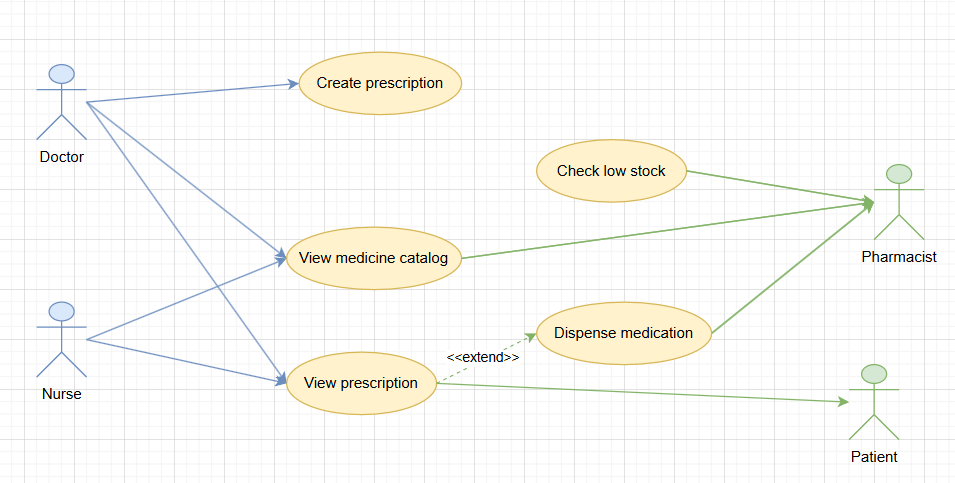
\includegraphics[width=1\linewidth]{images/use-case-diagram-pharmacy.png}
    \caption{Use case diagram - Prescription \& Pharmacy}
    \label{fig:usecasepharmacy}
\end{figure}

\subsubsection{Use case table}


\begin{table}[H]
\centering
\begin{tabular}{|l|p{9cm}|}
\hline
\textbf{Name} & \textbf{Description} \\
\hline
Actor & Pharmacist \\
\hline
Main function & Dispense Medication \\
\hline
Brief description & The Pharmacist selects a prescription that is in APPROVED status, verifies patient allergies and medicine stock, then confirms the dispense action. The system updates the prescription status to DISPENSED, records the dispenser and timestamp, deducts the quantity from inventory, and creates an inventory transaction (OUT). \\
\hline
Context information & Prescription exists and has been approved by a Doctor. Medicine is available in the pharmacy inventory. \\
\hline
Triggers & User must be authenticated and have the Pharmacist (or Admin) role. The prescription must be in APPROVED status. The requested medicine and quantity must be in stock. \\
\hline
\end{tabular}

\label{tab:uc-prescription-1}

\end{table}



\begin{table}[H]
\centering
\begin{tabular}{|l|p{9cm}|}
\hline
\textbf{Name} & \textbf{Description} \\
\hline
Flow of events summary & 
1. Pharmacist opens the list of approved prescriptions. \\
& 2. Pharmacist selects a prescription to dispense. \\
& 3. System validates authorization (PEP $\rightarrow$ PDP); if Deny, access is refused. \\
& 4. Pharmacist reviews prescription details and (if shown) patient allergies. \\
& 5. Pharmacist verifies that the medicine and quantity are available in stock. \\
& 6. Pharmacist confirms the dispense action. \\
& 7. System updates prescription status to DISPENSED and records dispensed\_by, dispensed\_at. \\
& 8. System deducts quantity from inventory and creates an OUT transaction. \\
& 9. System returns success to the Pharmacist. \\
\hline
\end{tabular}
\caption{Use case table: Dispense Medication (Prescription \& Pharmacy)}
\label{tab:uc-prescription}

\end{table}
\vspace{1em}


\subsubsection{Activity Diagram}

\begin{figure}[H]
    \centering
    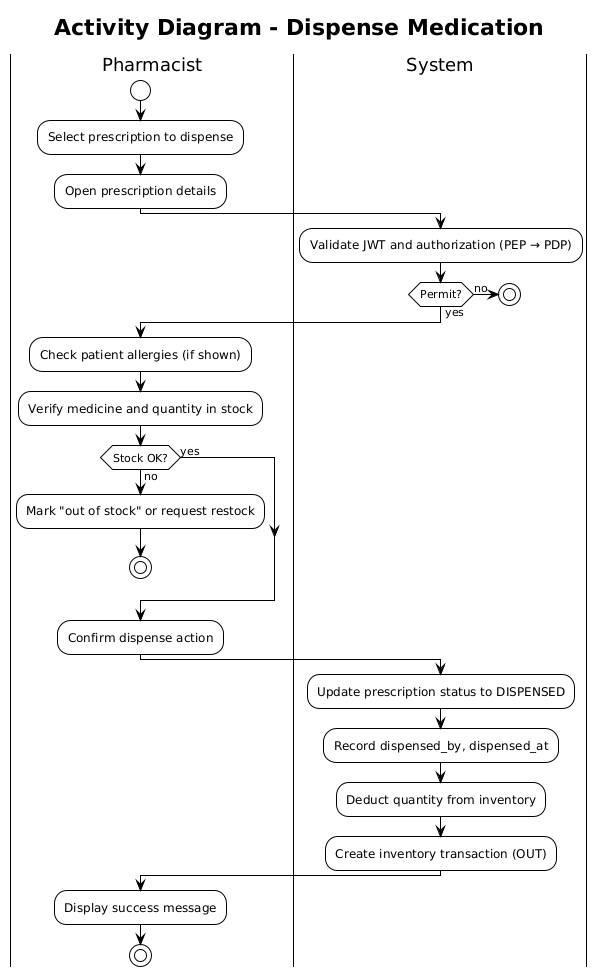
\includegraphics[width=0.5\linewidth]{images/actitvitypharmacy.png}
    \caption{Activity Diagram - Dispense Medication}
    \label{fig:activitypharmacy}
\end{figure}
A typical dispensing flow starts when the pharmacist opens the list of approved prescriptions and selects one to dispense. The system evaluates authorization before performing any updates. If permitted, the pharmacist verifies prescription details and stock availability, then confirms the dispensing action. The system updates the prescription status to \texttt{DISPENSED}, records the dispenser and timestamp, deducts the quantity from inventory, and creates an inventory transaction record. By placing authorization in front of these state changes, the system reduces the risk of unintended updates and keeps enforcement consistent.

\section{Hybrid Access Control Design}

\subsection{Model Selection}
In hospital systems, access control must balance two needs. First, patient data is highly sensitive, so access must be restricted and auditable. Second, clinical work is time-critical, so the model must remain practical to manage and fast enough for daily use. Traditional RBAC is widely used because it is easy to review and administer once roles and permissions are defined. However, RBAC alone becomes rigid when access depends on context such as time, shift, assignment, or department. When RBAC tries to cover many contexts by introducing more roles, it can lead to role explosion (too many roles to maintain). \cite{KuhnCoyneWeil2010, Ferraiolo2007RBAC2E}
\vspace{0.5cm}


ABAC is more flexible because it can express rules directly using attributes, but it can be difficult to manage at scale. \cite{KuhnCoyneWeil2010} points out that ABAC’s flexibility comes with a cost: many attribute combinations may need to be considered, and it can be hard to analyze “who has what permissions” for a given employee position.
\vspace{0.5cm}


To combine the strengths of both models, this thesis adopts RBAC-A (role-centric), as described by \cite{KuhnCoyneWeil2010}. In RBAC-A, roles still define the maximum permission set, while attributes are added as constraints. In the role-centric variant, attribute-based rules can only reduce the permissions available to a user; they do not expand access beyond what the role already allows.
\vspace{0.5cm}


\cite{KuhnCoyneWeil2010} summarize several integration options and describe the role-centric approach as the mapping:


\textbf{User → Role → Attributes → Permission decision }

Under this approach, the final permission set is computed as an intersection:

\begin{itemize}
    \item let \emph{P} be the set of permissions granted by active roles (RBAC baseline),
    \item let \emph{R} be the set of permissions allowed after applying attribute constraints (ABAC rules),
then the effective permissions are $P \cap $R
\end{itemize}
This is the key reason this thesis selects role-centric RBAC-A: it keeps RBAC’s administrative clarity (roles remain the main unit of review), while adding enough flexibility to handle common hospital contexts (time, department, owner, and so on). 

\subsection{Policy Evaluation Workflow (PEP–PDP–PIP)}
Figure~\ref{fig:peppippdp} summarizes how the prototype evaluates authorization decisions. The gateway acts as the PEP and intercepts each request. It validates the JWT and extracts basic claims such as user id and roles. The gateway then sends a decision request to the Authorization Service, which acts as the PDP. When the decision requires context beyond what the token contains, the PDP queries the PIP for additional attributes, for example to check whether a doctor is assigned to a patient. After collecting the required attributes, the PDP evaluates the policy using OPA and returns a Permit/Deny result. The gateway enforces the result by forwarding the request only when access is permitted. 


\begin{figure}[H]
    \centering
    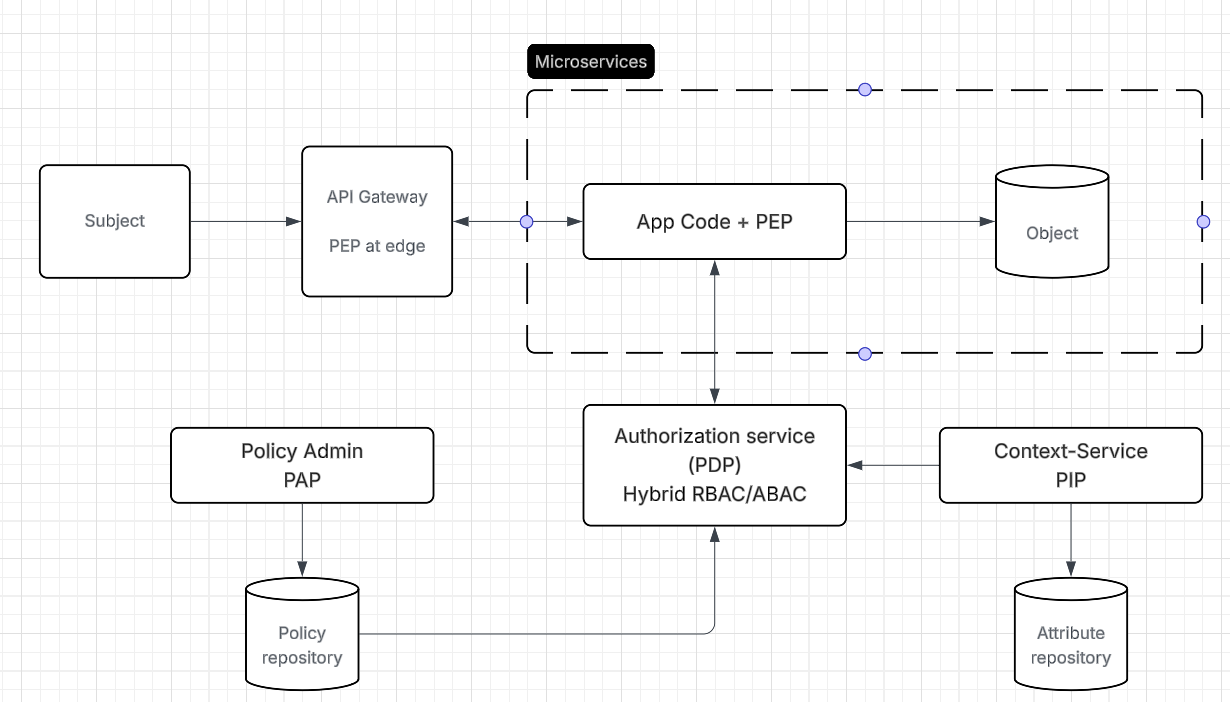
\includegraphics[width=0.75\linewidth]{images/peppippdp.png}
    \caption{System architecture for hybrid RBAC/ABAC authorization}
    \label{fig:peppippdp}
\end{figure}

This workflow protects business services consistently while keeping policy logic centralized and easier to maintain.

\subsection{Policy structure \& combining strategy}
Policies in this thesis follow the role-centric RBAC-A idea: roles define the baseline actions that are generally allowed on each resource type, and attributes narrow access through constraints such as time windows, department matching, or other context. The decision logic therefore happens in two stages. First, the system checks whether the user’s role allows the requested operation on the resource type. If the RBAC baseline fails, the request is denied immediately. If the RBAC baseline passes, the system evaluates ABAC constraints using the attributes collected through the PIP.
\vspace{0.5cm}


When more than one rule or policy can match a request, the system needs a clear and predictable combining behavior. In this thesis, matching rules are first evaluated within their parent policy according to that policy’s combining algorithm (e.g.\ \texttt{deny-overrides}, \texttt{allow-overrides}, or \texttt{first-applicable} based on priority). After that, the system resolves the final decision across matched rules using deterministic priority: deny rules take precedence; otherwise, the highest-priority allow rule wins. This separation keeps evaluation predictable while still allowing policies to be written in a practical format for administration and testing.

\subsection{Attribute model (Subject–Resource–Action–Context)}
\label{sec:hybrid-access-control-design}
The hybrid model in this thesis organizes attributes into four groups. Subject attributes represent who is making the request, such as user id, role, department, and staff-related fields. Resource attributes describe what data is being accessed, such as resource type, resource id, owner id, department id, or status fields that belong to domain objects. The action describes what operation is being requested, such as \texttt{read}, \texttt{create}, or \texttt{update}. Context attributes represent runtime conditions such as time or shift, device information, and IP or location indicators.
\vspace{0.5cm}

\paragraph{Reasons for the chosen attributes:}
The hybrid model in this thesis organizes attributes into four groups. Subject attributes represent who is making the request, such as user id, role, department, and staff-related fields. Resource attributes describe what data is being accessed, such as resource type, resource id, owner id, department id, or status fields that belong to domain objects. The action describes what operation is being requested, such as \texttt{read}, \texttt{create}, or \texttt{update}. Context attributes represent runtime conditions such as time or shift, device information, and IP or location indicators.
\vspace{0.5cm}


The PIP is responsible for collecting only the minimum attributes required to evaluate constraints. It should not return full business payloads, especially for sensitive resources. This design keeps authorization focused on decision-making while limiting unnecessary exposure of medical data.





\subsection{Policy conflict detection}
\label{sec:policy-conflict-detection}
When many policies are defined, some rules can apply to the same request but return different decisions. For example, one rule may allow access for a given role and resource in a time window, and another may deny the same. That situation is called a \emph{policy conflict}. If conflicts are not detected, the system can behave in an unpredictable way: the same kind of request might be allowed or denied depending on the order of evaluation or the combining algorithm. In practice, security problems often come from wrong or inconsistent policy configuration rather than from cryptographic failures~\cite{Zheng2019ABAC}. So we need a way to find conflicts before or after policy changes. The idea is simple: (1) find pairs of rules whose conditions can overlap (i.e.\ there exists at least one request that matches both), and (2) among those, report pairs where one rule permits and the other denies. The result is a list of conflicting rule pairs that an administrator can review and fix.
\vspace{0.5cm}

Because the number of rules can be large, comparing every pair of rules is expensive. Two approaches from the literature help. The first is \emph{rule reduction}: drop or ignore rules that cannot take part in any conflict (e.g.\ rules without actions or without subject/object attributes), and only run conflict checks on the remaining set~\cite{Shu2009Conflicts}. The second is to encode each rule (or its attribute conditions) into a compact form and use fast operations to test overlap.\cite{Zheng2019ABAC} represents attribute conditions as binary sequences and use bitwise AND to detect overlap between two rules, which speeds up conflict detection when the policy set and the number of attributes grow.
\vspace{0.5cm}


In this thesis, conflict detection is implemented in the policy service. When an administrator adds or updates policies, the system can run a conflict check (on demand or after save). The implementation uses rule reduction: only rules that have actions and at least subject or object attributes are considered. Rules are grouped by resource type and action so that we only compare rules that share at least one action and can apply to the same resource type. For each candidate pair (one Allow, one Deny), the service checks whether their subject and object attribute sets overlap; if time conditions are present, it also checks whether their time intervals overlap, using a binary-search style check on disjoint time intervals. In addition, \emph{redundancy} is detected: two rules with the same effect (both Allow or both Deny) that have fully overlapping conditions. Redundancy does not change the decision but makes the policy set harder to maintain; reporting it helps the administrator simplify policies~\cite{Zheng2019ABAC}. The output of the detector is a list of conflicting pairs (and optionally a ``witness'' request that matches both rules), so the admin can adjust or merge rules and redeploy.

\subsection{Policy governance and misuse prevention}
\label{sec:policy-governance}

The role-centric hybrid model in this thesis helps address the practical problem of role explosion. However, a hybrid system also introduces a second class of risks: \textbf{policy governance risks}. If policy changes are not controlled, hybrid rules can become inconsistent over time, and privileged users can abuse their power by creating overly broad Allow rules or by weakening constraints and conditions during policy updates. In a hospital setting, this is serious because the most harmful failures are \emph{false-permit} decisions (access granted when it should have been denied).
\vspace{0.5cm}

This thesis therefore treats governance as part of the access control design. The goal is to keep authorization behavior predictable, make policy changes traceable, and reduce the chance that a single administrator action silently weakens security. To address the concern that hybrid (RBAC \& ABAC) implementation must be \emph{effectively controlled}---and not only mentioned---we define what constitutes misuse and how the following controls prevent it.
\vspace{0.5cm}

\paragraph{Misuse and abuse in this context.}
We define \textbf{policy misuse} or \textbf{abuse of power} in the hybrid system as: (i) introducing into the enabled policy set a pair of rules that form an \emph{authorization conflict} (one Allow and one Deny for the same request conditions, as in Section~\ref{sec:policy-conflict-detection}), which makes access behavior unpredictable; or (ii) allowing policy write operations by subjects who are not authorized to administer policies, so that the system cannot attribute or limit who changes rules. The governance controls below are designed so that (i) is prevented by conflict checks on update, and (ii) is prevented by restricting policy writes to administrators.
\vspace{0.5cm}

\paragraph{Invariants and policy-update conditions.}
The design maintains two invariants. \textbf{Conflict-freedom:} at every point in time, the set of enabled policies does not contain any pair of rules that form an AUTH\_CONFLICT (overlapping conditions with opposite effects). \textbf{Write-restriction:} only subjects with the ADMIN role may perform create, update, or delete on policies. For a \emph{policy update} (create or update), the pre-condition is: the subject has role ADMIN; and, when conflict-on-save is enabled in strict mode, the proposed policy set (existing enabled plus the new or updated policy) must not contain any AUTH\_CONFLICT. The post-condition after a successful save is that the conflict-freedom invariant holds and the policy record has updated version, timestamps, and administrator identity (created\_by / updated\_by) for traceability.
\vspace{0.5cm}

\subsubsection*{Deterministic decision semantics (avoid ambiguous behavior)}
The first governance control is making the decision semantics explicit. In this thesis, evaluation is deterministic in two ways. First, the system follows the role-centric RBAC-A principle: ABAC constraints \emph{only narrow} access. If the RBAC baseline does not allow an action for the role, the request is denied immediately. Second, when multiple rules can match, the policy engine applies a defined combining strategy (e.g. \texttt{deny-overrides}, \texttt{allow-overrides}, or \texttt{first-applicable} within a policy), and then resolves the final result using a clear precedence: deny rules take priority; otherwise, the highest-priority allow rule applies. This reduces the risk of ``accidental permission'' caused by unclear rule ordering and supports predictable behavior so that misuse (e.g.\ unintended broadening of access) is easier to detect and audit.
\vspace{0.5cm}

\subsubsection*{Restricted policy administration (limit who can change rules)}
The second control is limiting who can create or update policies. In the prototype, policy write operations are restricted to administrators. This directly enforces the write-restriction invariant and prevents abuse by non-admin users (only ADMIN can change rules). This includes creating policies, updating policies, triggering OPA synchronization, and running conflict detection. Read-only access (listing and viewing policies) can be granted more widely for transparency, but write access is treated as a privileged action.
\vspace{0.5cm}

This separation matters because policy administration is a powerful capability. If too many users can edit policies, the system becomes hard to control and easy to misuse.
\vspace{0.5cm}

\subsubsection*{Change traceability and policy version history}
Hybrid systems evolve. New endpoints are added, services change, and hospital workflows change. For that reason, policy governance must support traceability. In this thesis, policies are stored with metadata that supports auditing and rollback: \texttt{enabled} state, \texttt{version}, timestamps, and the administrator identity (created/updated by). Metadata (e.g.\ \texttt{created\_at}, \texttt{updated\_at}, \texttt{created\_by\_keycloak\_id}, \texttt{updated\_by\_keycloak\_id}) creates a clear trail of \emph{who changed what and when}, which is necessary when investigating incidents or reviewing why access changed after a deployment. Full content snapshots for each version can be added in future work to support rollback; the current prototype relies on version and actor metadata for accountability.
\vspace{0.5cm}

\subsubsection*{Conflict checks on policy update (fail safe by default)}
The most direct way to control conflict risk is to detect it at the time of change. In this prototype, conflict detection is not only a reporting tool; it is also used as a guardrail. Before saving a new or updated policy, the policy service runs conflict detection on the proposed state (existing enabled rules plus the proposed change) when configured in \emph{strict} mode. If the change introduces an authorization conflict (Allow/Deny overlap on the same action and resource type under overlapping attribute conditions), the update is \textbf{rejected} and the service returns HTTP 409 with a conflict report; no change is persisted, so the conflict-freedom invariant is preserved. This prevents administrators from accidentally publishing policies that make access behavior unpredictable and directly addresses misuse (i).
\vspace{0.5cm}

This ``conflict-on-save'' approach is intentionally conservative. It prefers a safe failure (do not apply risky policy changes) over silently deploying a policy set with unclear behavior.
\vspace{0.5cm}

\subsubsection*{Audit evidence for sensitive access and privileged operations}
Finally, governance requires evidence. The authorization path records audit information for protected requests, including the final Permit/Deny decision and the context used for evaluation. For privileged events (for example policy updates, conflict scans, or access to audit logs), audit data is especially important because it supports accountability and later review. Policy create/update events can be sent to the audit service so that every change to the policy set is logged; this closes the loop from governance design to observable evidence.
\vspace{0.5cm}

In summary, the hybrid RBAC/ABAC rules in this thesis are intentionally kept manageable, but they are also surrounded by governance controls that \emph{solve} the problems of conflict and abuse: deterministic combining avoids ambiguous decisions; restricted administration enforces write-restriction; version and actor metadata provide traceability; conflict-on-save enforces conflict-freedom; and audit evidence supports accountability. Thus the hybrid model is kept safe in practice by controlling policy evolution both in design (Section~\ref{sec:policy-governance}) and in the prototype (Chapter~4).
\section{Policy Model}
\label{sec:policy-model}

This section describes the data and structural model used for policies and audit in the HMS: the RBAC baseline, the ABAC constraint layer, the policy and rule schema, the policy store (PAP), and the audit log model. These elements support the workflow and attribute model described in Section~\ref{sec:hybrid-access-control-design}.

\subsection{RBAC model}
\label{sec:rbac-model}

The RBAC layer defines the baseline permissions. Each user is assigned one or more roles (e.g.\ DOCTOR, NURSE, RECEPTIONIST, PHARMACIST, ADMIN) by the Identity Provider (Keycloak). Roles are carried in the JWT and passed to the PDP. The policy engine (OPA) evaluates whether the requested action is permitted for the user's role on the given resource type. A role hierarchy is supported in policy: for example, PRIMARY\_DOCTOR is treated as having DOCTOR permissions, and administrative roles (Admin, admin) are normalized to ADMIN so that a single role check can be used in Rego. Thus the RBAC model in this thesis is: \emph{user $\rightarrow$ roles (from IdP) $\rightarrow$ permitted (resource\_type, action)}; the PDP allows an action only if the role is in the set of roles permitted for that resource and action.

\subsection{ABAC constraint model}
\label{sec:abac-constraint-model}
ABAC constraints narrow the RBAC baseline. Each policy rule can specify subject attributes (e.g.\ role, department\_id), resource attributes (e.g.\ resource type, owner\_id, department\_id, status), and optional conditions (e.g.\ time windows, IP range). In the implementation, a rule is stored with \texttt{effect} (Allow or Deny), \texttt{subjects}, \texttt{actions}, \texttt{resources} (each as JSON), and \texttt{conditions} (JSON). The PDP builds an input object that includes the subject (from JWT and optional PIP), the resource (type and attributes), and the action; OPA then evaluates constraint predicates such as same-department, same-hospital, owner-is-user, allowed status, and time-window. Thus the ABAC model is: \emph{given an RBAC-allowed (role, resource\_type, action), the request is permitted only if all applicable attribute constraints are satisfied}.


\subsection{Policy model and JSON schema}

In this thesis, a policy is treated as a named container that groups rules under a defined combining behavior. Each rule includes an effect (Allow/Deny), subject constraints (as JSON), actions (as a list), resource constraints (as JSON), optional conditions (as JSON), and a priority field. The policy itself also stores its combining algorithm. The combining algorithm can be deny-overrides, allow-overrides, or first-applicable, depending on the intended behavior of that policy. Policies are stored in the policy store and normalized into a format that OPA can consume during evaluation. Figure~\ref{lst:policy-json} shows a sample policy using the JSON format exposed by the Policy Service API, including examples of time-range and IP constraints. With deny-overrides, any request matching a deny rule results in Deny even if other allow rules exist.
\vspace{0.5cm}

Before encoding rules into the Policy Service JSON format and deploying them to OPA, the system states the intended access
control rules in plain language so that they are easy to review. Doctors may read or update a patient record, but only when
the request is made within working hours and the doctor’s department matches the patient record’s department. Even when
that access would normally be allowed, it must be denied when the request comes from a blocked network range. Nurses may
update patient-related information within their hospital scope, but their access is still constrained by department and
other context rules. Receptionists may create appointments, but they must not read patient medical records. Pharmacists may
dispense prescriptions, but only when the prescription is in the correct state and the request is within the hospital
scope. Administrators may manage policies and audit functions, while external auditors may only read audit logs. These
plain-English rules are then translated into structured fields (\texttt{subjects}, \texttt{actions}, \texttt{resources}, and
\texttt{conditions}) and evaluated with the selected combining algorithm (e.g.\ \texttt{deny-overrides}) so that Deny rules
can override Allow rules when both match. Table~\ref{tab:access-control-rules-plain} lists all access control rules for the hospital example in plain English.

\begin{table}[H]
\centering
\renewcommand{\arraystretch}{1.2}
\small
\begin{tabular}{|l|p{5.2cm}|p{5.8cm}|}
\hline
\textbf{Role} & \textbf{Rule (plain English)} & \textbf{Conditions / exceptions} \\
\hline
Doctor & May view patient records and medical history. & Only when the doctor's department matches the patient record's department. \\
\cline{2-3}
Doctor & May read and update patient records. & Only when same department and within working hours (e.g.\ 08:00--17:00). \\
\cline{2-3}
Doctor & Must not delete patient records. & Deny rule: delete on patient records is always denied for doctors. \\
\cline{2-3}
Doctor, Nurse & Must not access patient records with critical sensitivity. & Deny when user's position level is below 3 (e.g.\ junior staff). \\
\cline{2-3}
Doctor & Must not access patient records from a blocked network. & Deny when the request comes from a blocked IP range (e.g.\ external/untrusted range). \\
\hline
Nurse & May view and update vital signs (medical history). & Only within hospital scope; may be constrained by department or ward. \\
\hline
Lab technician & May view, update lab orders and create lab results. & Only for lab orders assigned to that technician; within hospital scope. \\
\hline
Pharmacist & May read, create, update, and delete medicines. & Only within the same hospital. \\
\cline{2-3}
Pharmacist & May read, create, update, and delete prescriptions (e.g.\ dispense). & Only within the same hospital; prescription in correct state when required. \\
\hline
Receptionist & May create appointments. & Subject to hospital/department context as configured. \\
\cline{2-3}
Receptionist & Must not read patient medical records. & No permission for patient record or medical history read. \\
\hline
Patient & May read own patient record. & Only when requesting ``own'' record (e.g.\ \texttt{GET /api/patients/me}) with no resource id. \\
\hline
Administrator & May perform any action on any resource (full access). & No ABAC constraints for general admin access. \\
\cline{2-3}
Administrator & May manage policies (create, update, delete, sync to OPA). & Policy administration restricted to ADMIN role. \\
\cline{2-3}
Administrator & May read and clear (delete) audit logs. & Only ADMIN may clear or delete audit logs. \\
\hline
External auditor & May read audit logs only. & Read-only; cannot modify policies or clear audit data. \\
\hline
\end{tabular}
\caption{Access control rules for the hospital example in plain English. Allow rules may be narrowed by conditions; Deny rules override Allow when both match (deny-overrides).}
\label{tab:access-control-rules-plain}
\end{table}

\vspace{0.5cm}

A sample policy in the JSON format used by the Policy Service API is given in Figure~\ref{lst:policy-json}. Conditions are shown in the \emph{attribute-based tree} form produced by the policy UI: user and resource attributes (e.g.\ \texttt{user.attributes.departmentId}, \texttt{resource.departmentId}) and environment attributes (e.g.\ \texttt{env.time}) are combined with \texttt{AND}. Rule r1 allows doctors to read/update patient records when the user's department matches the resource's department (\texttt{value\_ref} compares two attributes) and the request time is in the range 08:00--17:00; r2 illustrates a deny constraint on \texttt{env.ip} (blocked network range). With \texttt{deny-overrides}, any request matching the Deny rule is denied.

\begin{figure}[H]
\centering
\small
\begin{verbatim}
{
  "tenantId": "HOSPITAL_A",
  "policyId": "policy-doctor-patient-record",
  "policyName": "Doctor access to patient records",
  "description": "Allow doctors read/update in same department, within working hours",
  "combiningAlgorithm": "deny-overrides",
  "priority": 10,
  "enabled": true,
  "rules": [
    {
      "ruleId": "r1",
      "ruleName": "Allow same-department and working hours",
      "effect": "Allow",
      "subjects": {"roles": ["DOCTOR"]},
      "actions": ["read", "update"],
      "resources": {"type": "patient_record"},
      "conditions": {
        "operator": "AND",
        "children": [
          {
            "field": "resource.departmentId",
            "operator": "eq",
            "value_ref": "user.attributes.departmentId"
          },
          {"field": "env.time", "operator": "eq", "value": "08:00-17:00"}
        ]
      },
      "priority": 1
    },
    {
      "ruleId": "r2",
      "ruleName": "Deny from blocked network range",
      "effect": "Deny",
      "subjects": {"roles": ["DOCTOR"]},
      "actions": ["read", "update"],
      "resources": {"type": "patient_record"},
      "conditions": {
        "operator": "AND",
        "children": [
            {"field": "env.ip", "operator": "eq", "value": "203.0.113.0/24"}]
      },
      "priority": 2
    }
  ]
}
\end{verbatim}
\caption{Sample policy JSON with attribute-based conditions}
\label{lst:policy-json}
\end{figure}



\subsection{Policy store and policy administration data}
\label{sec:policy-store}

Policies and rules are persisted in a relational database (MySQL) owned by the Policy Service. The \texttt{policies} table stores policy metadata such as identifier, name, combining algorithm, enable flag, priority, versioning information, and timestamps. The \texttt{policy\_rules} table stores individual rule entries including effect, JSON fields for subject/action/resource/conditions, priority, and enable flag.

\vspace{0.5cm}

To make the schema concrete, Table~\ref{tab:policy-service-examples} shows example rows for a hospital rule set. The example encodes a policy container that uses \texttt{deny-overrides} and two fine-grained rules: an allow rule for doctors under scope and working-hours constraints, and a deny rule as an exception for a blocked IP range. This type of representation demonstrates how the schema can capture multiple rules that may overlap, while leaving the final resolution to the combining strategy enforced by the policy engine.

\begin{table}[H]
\centering
\renewcommand{\arraystretch}{1.15}
\small
\begin{tabular}{|p{2.4cm}|p{3.8cm}|p{9.0cm}|}
\hline
\textbf{Entity} & \textbf{Field} & \textbf{Example value} \\
\hline
\texttt{policies} & \texttt{tenant\_id} & \texttt{"HOSPITAL\_A"} \\
\cline{2-3}
& \texttt{policy\_id} & \texttt{"policy-doctor-emr"} \\
\cline{2-3}
& \texttt{policy\_name} & \texttt{"Doctor access to patient records"} \\
\cline{2-3}
& \texttt{combining\_algorithm} & \texttt{"deny-overrides"} \\
\cline{2-3}
& \texttt{priority} & \texttt{10} \\
\cline{2-3}
& \texttt{enabled} & \texttt{true} \\
\hline

\texttt{policy\_rules} (r1) & \texttt{rule\_id} & \texttt{"r1-allow-doctor-read-update"} \\
\cline{2-3}
& \texttt{effect} & \texttt{"allow"} \\
\cline{2-3}
& \texttt{priority} & \texttt{10} \\
\cline{2-3}
& \texttt{subjects} & \texttt{\{"roles":["DOCTOR"]\}} \\
\cline{2-3}
& \texttt{actions} & \texttt{["read","update"]} \\
\cline{2-3}
& \texttt{resources} & \texttt{\{"type":"patient\_record"\}} \\
\cline{2-3}
& \texttt{conditions} &
\texttt{\{"same\_department":true,"same\_hospital":true,"working\_hours\_only":true\}} \\
\hline

\texttt{policy\_rules} (r2) & \texttt{rule\_id} & \texttt{"r2-deny-blocked-ip-range"} \\
\cline{2-3}
& \texttt{effect} & \texttt{"deny"} \\
\cline{2-3}
& \texttt{priority} & \texttt{100} \\
\cline{2-3}
& \texttt{subjects} & \texttt{\{"roles":["DOCTOR"]\}} \\
\cline{2-3}
& \texttt{actions} & \texttt{["read","update"]} \\
\cline{2-3}
& \texttt{resources} & \texttt{\{"type":"patient\_record"\}} \\
\cline{2-3}
& \texttt{conditions} & \texttt{\{"allowed\_ip\_ranges":["203.0.113.0/24"]\}} \\
\hline
\end{tabular}
\caption{Example policy and rule rows stored in MySQL for the hospital scenario. Conditions use the flat JSON form supported by the Policy Service and OPA transformer (same department/hospital, working hours; deny when IP in blocked range).}
\label{tab:policy-service-examples}
\end{table}

\vspace{0.5cm}

In the implementation, the Policy Service retrieves only enabled policy containers and enabled rules, normalizes their JSON structure into the expected input format of the OPA engine, and publishes them to OPA as dynamic data (e.g., \texttt{data.dynamic\_policies}). This supports policy administration (create/update/disable) while keeping authorization rules flexible enough for ABAC constraints in the hybrid RBAC/ABAC model.

\vspace{0.5cm}

Admins manage policies through the Policy Service API (PAP), including creating and updating policies and rules. After changes, the Policy Service publishes a normalized policy set to OPA, for example through a bundle or REST-based update. This keeps the policy database as the single source of truth, while OPA holds a deployed copy used only for evaluation.


\subsection{Audit log model}
\label{sec:audit-log-model}

Hospital systems require traceability because access to medical and financial data must be accountable. For this reason, authorization decisions and important actions are recorded by the Audit Service. The audit model captures what happened (event type), who performed it (actor identifier and role), what was accessed (resource type and resource id), the requested action, the decision outcome, and supporting metadata such as timestamp and correlation identifiers. In the prototype, the gateway or PDP emits an audit event and the Audit Service persists it in an \texttt{audit\_logs} table. Indexing common fields such as actor id, resource type, resource id, and timestamp supports later filtering and reporting. This structure makes it possible to answer a practical set of questions: who did what, on which data, when, and with what outcome.



\section{Technology Stack}
\label{sec:technology-stack}

This section summarizes the technologies used to implement the hospital management system and its hybrid RBAC-ABAC authorization layer. The stack is organized by role: backend services, frontend, identity and policy engines, data storage, messaging, and infrastructure.

\subsection{Backend and API Gateway}
Microservices are implemented with Java 21 and Spring Boot (3.2.0). The API Gateway is Spring Cloud Gateway (Spring Cloud 2023.0.0), which handles routing, JWT validation (OAuth2 Resource Server), and acts as the Policy Enforcement Point (PEP). Backend services use Spring Web (REST), Spring Data JPA for persistence, and Spring Security with OAuth2 Resource Server for validating tokens issued by Keycloak. This choice provides a mature, standard way to integrate with an external IdP and to enforce authorization at the gateway before requests reach domain services.

\subsection{Identity and policy engines}
Keycloak (24.0) is used as the Identity Provider (IdP): it manages users, roles, and realms and issues JWT access tokens. The Policy Decision Point (PDP) relies on Open Policy Agent (OPA) as the policy engine. Policies are written in Rego and can be loaded from files or via bundle API; the authorization service builds the input (subject, resource, action, attributes) and calls OPA's HTTP API to obtain Allow/Deny decisions. This separation keeps authorization logic declarative and auditable.

\subsection{Data and messaging}
MySQL 8.0 is the primary database; each service uses its own schema or database for isolation. RabbitMQ (3.0, with management plugin) is used for asynchronous events such as audit logging and notifications, enabling loose coupling between the PDP, domain services, and the audit service. Redis is available for rate limiting, session and caching use at the gateway.

\subsection{Frontend}
The user interface is built with Next.js (14), React 18, and TypeScript. Authentication is integrated with Keycloak via NextAuth. The UI uses Tailwind CSS for styling and Recharts for dashboards; role-specific views (receptionist, doctor, pharmacist, admin, etc.) call backend APIs through the gateway, so all authorization is enforced at the PEP/PDP layer rather than in the browser.

Table~\ref{tab:tech-stack} summarizes the main components and their versions or families. The implementation and deployment use Docker and Docker Compose for Keycloak, OPA, MySQL, RabbitMQ, and Redis; microservices can run on the host or in containers.

\begin{table}[H]
\centering
\label{tab:tech-stack}
\begin{tabular}{|l|l|l|}
\hline
\textbf{Category} & \textbf{Technology} & \textbf{Version / notes} \\
\hline
Runtime & Java & 21 \\
Backend framework & Spring Boot & 3.2.0 \\
API Gateway & Spring Cloud Gateway & 2023.0.0 \\
Identity (IdP) & Keycloak & 24.0 \\
Policy engine & Open Policy Agent (OPA) & Rego, HTTP API \\
Database & MySQL & 8.0 \\
Messaging & RabbitMQ & 3.0 (management plugin) \\
Cache / rate limit & Redis & 7.0 \\
Frontend & Next.js, React, TypeScript & 14, 18, 5.0 \\
Auth (frontend) & NextAuth & 4.0 \\
Containers & Docker, Docker Compose & — \\
\hline
\end{tabular}
\caption{Technology stack overview.}
\label{tab:tech-stack}
\end{table}

The technology choices support the architecture described in Section~\ref{sec:sysarchitecture}: a central PDP (authorization service + OPA), a single PEP at the gateway, and optional attribute enrichment via the user service, with policies managed and checked for conflicts in the policy service before being deployed to OPA.
\vspace{0.5cm}

To summarize, the system design uses a single enforcement point at the gateway and a centralized PDP for consistent decisions across microservices. The hybrid model is role-centric: roles grant the maximum permissions and ABAC constraints narrow them based on context and resource attributes. Attributes are fetched via PIP from domain services without sharing databases. The next chapter explains how these components are implemented and validated in the demo.

\chapter{Implementation \& Evaluation}
\label{chap:implementaion}
\section{Implementation Overview}
This chapter presents how the proposed hospital management system (HMS) and the hybrid authorization layer are implemented. The prototype follows a microservices style. Each business service owns its database schema and exposes REST APIs. All external requests go through a single gateway. The gateway acts as the Policy Enforcement Point (PEP). It calls a dedicated Authorization Service that acts as the Policy Decision Point (PDP). The PDP evaluates role-centric RBAC-A policies, where roles define the baseline permissions and attributes are used as constraints to narrow access.
\vspace{0.5cm}

The goal of this chapter is twofold. First, it explains the implementation choices and data structures that support authorization. Second, it describes how this implementation can be tested and evaluated using clear scenarios and measurable metrics.

\subsection{Implemented components}

\begin{itemize}
    \item \textbf{Client/UI:} A web UI supports role-specific workflows such as receptionist booking,
    doctor confirmation, pharmacist dispensing, and admin policy management. The UI calls backend
    APIs only through the gateway. It does not perform authorization logic in the browser.

    \item \textbf{API Gateway / BFF (PEP):} The gateway is the single entry point for client requests.
    It validates JWT tokens issued by the Identity Provider, extracts basic claims (user id, roles, and
    optional tenant fields), and enforces the final decision. For protected endpoints, the gateway sends
    a decision request to the PDP before forwarding traffic to business services.

    \item \textbf{Authorization Service (PDP):} The PDP receives decision requests from the gateway.
    It normalizes the request, enriches it with attributes through the PIP when needed, and calls OPA
    to evaluate policy rules. The PDP returns a compact Permit/Deny decision to the gateway.

    \item \textbf{OPA policy engine:} Open Policy Agent (OPA) evaluates authorization logic written
    in Rego. This keeps policy evaluation separate from business code and makes rules easier to review
    and update.

    \item \textbf{Policy Service (PAP + Policy Store):} Administrators manage policies via the Policy
    Service. Policies and rules are stored in a dedicated policy database. After updates, the service
    publishes the normalized policy set to OPA.

    \item \textbf{Attribute Provider (PIP):} The PIP collects attributes required by policies. It queries
    domain services (for example, user department, appointment department, or patient sensitivity) and
    returns only the fields needed for the decision. It does not return full business payloads.

    \item \textbf{Business microservices:} The prototype focuses on six services: User, Patient,
    Appointment, Lab, Pharmacy, and Billing. Each service owns its database schema and exposes REST
    APIs.

    \item \textbf{Audit Service:} The system records security and access events for traceability. Audit
    logs are written asynchronously to reduce latency on the main request path.
\end{itemize}

This structure follows the design in Chapter 3. The key difference is that this chapter describes how the design is implemented in code and data models.

\subsection{End-to-end request flow}

A typical protected request follows these steps:

\begin{enumerate}
    \item The client calls an API endpoint through the gateway with a JWT in the \texttt{Authorization}
    header.

    \item The gateway validates the token and maps the HTTP request to an authorization request
    (subject, action, resource, and basic context).

    \item The gateway calls the PDP. If the policy requires extra context, the PDP requests additional
    attributes via the PIP.

    \item The PDP calls OPA and receives an Allow/Deny result (and optional metadata such as the matched rule).

    \item The gateway enforces the decision: it forwards the request on Permit, or returns
    \texttt{403 Forbidden} on Deny.

    \item The system records an audit event asynchronously for monitoring and investigation.
\end{enumerate}

This flow keeps business services focused on domain logic. Authorization decisions are evaluated in one place and enforced consistently at the edge.
\section{Database Design}
This section describes the database design used in the prototype. The system follows a \emph{database-per-service} approach. Each microservice owns its schema and can evolve it independently. The schemas are designed to support two needs:

\begin{itemize}
  \item \textbf{Business workflows:} appointments, prescriptions, billing, and staff/patient management.
  \item \textbf{Authorization and audit:} storing policy rules, and recording security-relevant actions.
\end{itemize}

All schemas are implemented in MySQL. The following subsections summarize the tables and key columns for each service, as shown in Tables~4.1--4.7.


\subsection{User Service — hospital\_users}
The User Service stores staff profiles and organizational structure. It also acts as a main source of staff attributes used by authorization (e.g., department and position level). Table~4.1 summarizes the schema.
\begin{table}[H]
\centering
\renewcommand{\arraystretch}{1.2}
\begin{tabular}{|p{3.2cm}|p{5.6cm}|p{5.6cm}|}
\hline
\textbf{Table} & \textbf{Purpose} & \textbf{Key columns} \\
\hline
\texttt{users} &
Common users linked with Keycloak &
\texttt{user\_id} (PK), \texttt{keycloak\_user\_id} (UNIQUE), \texttt{email}, \texttt{phone\_number}, \texttt{created\_at}, \texttt{updated\_at} \\
\hline
\texttt{departments} &
Hospital departments &
\texttt{department\_id} (PK), \texttt{name}, \texttt{location}, \texttt{hospital\_id}, \texttt{creation\_date}, \texttt{updation\_date} \\
\hline
\texttt{doctors} & Entity created for user who is
Doctor (DOCTOR) &
\texttt{doctor\_id} (PK), \texttt{user\_id} (FK \textrightarrow{} users), \texttt{first\_name}, \texttt{last\_name}, \texttt{gender}, \texttt{field}, \texttt{department\_id} (FK), \texttt{hospital\_id}, \texttt{position\_level}, \texttt{is\_active}\\
\hline
\texttt{nurses} &
Entity created for user who is Nurse (NURSE) &
\texttt{nurse\_id} (PK), \texttt{user\_id} (FK), \texttt{first\_name}, \texttt{last\_name}, \texttt{gender}, \texttt{department\_id} (FK), \texttt{hospital\_id}, \texttt{position\_level}, \texttt{is\_active} \\
\hline
\texttt{admins} &
Entity created for user who is Admin (ADMIN) &
\texttt{admin\_id} (PK), \texttt{user\_id} (FK), \texttt{first\_name}, \texttt{last\_name}, \texttt{gender}, \texttt{hospital\_id}, \texttt{admin\_level}, \texttt{created\_at} \\
\hline
        \texttt{pharmacists} &
    Entity created for user who is Pharmacist (PHARMACIST) &
    \texttt{pharmacist\_id} (PK), \texttt{user\_id} (FK), \texttt{hospital\_id}, \texttt{license\_number}, \texttt{is\_active} \\
    \hline
    \texttt{receptionists} &
    Entity created for user who is Receptionist (RECEPTIONIST) &
    \texttt{receptionist\_id} (PK), \texttt{user\_id} (FK), \texttt{hospital\_id}, \texttt{is\_active} \\
    \hline
    \texttt{billing\_clerks} &
    Entity created for user who is Billing clerk (BILLING\_CLERK) &
    \texttt{billing\_clerk\_id} (PK), \texttt{user\_id} (FK), \texttt{hospital\_id}, \texttt{is\_active} \\
    \hline
    \texttt{lab\_technicians}  & Entity created for user who is Lab Technician (LAB\_TECH) & \texttt{lab\_tech\_id (PK)}, \texttt{user\_id (FK)}, \texttt{department\_id (FK)}, \texttt{hospital\_id}, \texttt{is\_active}\\
    \hline
    \texttt{external\_auditor} & Entity created for user who is External Auditor (EXTERNAL\_AUDITOR) & \texttt{external\_auditor\_id (PK)}, \texttt{user\_id (FK)}, \texttt{department\_id (FK)}, \texttt{hospital\_id}, \texttt{is\_active}\\
    \hline
\hline
\end{tabular}
\label{tab:db-schema-user-service}
\caption{Database schema for User Service (\texttt{hospital\_users}).}
\end{table}
\begin{itemize}
  \item \textbf{\texttt{users}} links application users to Keycloak via \texttt{keycloak\_user\_id} (unique).
  \item \textbf{\texttt{departments}} stores hospital departments and location metadata.
  \item \textbf{Role-specific tables} store staff profiles by role:
  \texttt{doctors}, \texttt{nurses}, \texttt{admins}, \texttt{lab\_technicians},
  \texttt{pharmacists}, \texttt{receptionists}, \texttt{billing\_clerks}.
\end{itemize}
The role-specific tables reference \texttt{users} via \texttt{user\_id} (FK). This keeps login identity separated from staff profile data while still allowing stable joins when the PIP needs staff attributes.



\subsection{Patient Service — hospital\_patients}
The Patient Service stores patient identity and basic health history. Table~4.2 summarizes the schema.

\begin{table}[H]
\centering
\renewcommand{\arraystretch}{1.2}
\begin{tabular}{|p{3.2cm}|p{5.6cm}|p{5.6cm}|}
\hline
\textbf{Table} & \textbf{Purpose} & \textbf{Key columns} \\
\hline
\texttt{patients} &
Entity created for user who is Patient &
\texttt{patient\_id} (PK), \texttt{firstname}, \texttt{lastname}, \texttt{birthday}, \texttt{gender}, \texttt{phone\_number}, \texttt{keycloak\_user\_id} (UNIQUE), \texttt{hospital\_id} \\
\hline
\texttt{medical\_history} &
Medical history &
\texttt{id} (PK), \texttt{patient\_id} (FK \textrightarrow{} patients), \texttt{blood\_pressure}, \texttt{blood\_sugar}, \texttt{weight}, \texttt{height}, \texttt{creation\_date} \\
\hline
\end{tabular}
\caption{Database schema for Patient Service (\texttt{hospital\_patients}).}
\label{tab:db-schema-patient-service}
\end{table}
\begin{itemize}
  \item \textbf{\texttt{patients}} stores patient profile fields and links to Keycloak using \texttt{keycloak\_user\_id} (unique).
  \item \textbf{\texttt{medical\_history}} stores a minimal set of history/vitals and references \texttt{patients} via \texttt{patient\_id} (FK).
\end{itemize}

In the authorization flow, patient-related attributes can be fetched from this service (e.g., patient hospital id, or other context fields).


\subsection{Appointment Service — hospital\_appointments}
The Appointment Service stores scheduling information and appointment state transitions. Table~4.3 summarizes the schema.

\begin{table}[H]
\centering
\renewcommand{\arraystretch}{1.2}
\begin{tabular}{|p{3.2cm}|p{5.6cm}|p{5.6cm}|}
\hline
\textbf{Table} & \textbf{Purpose} & \textbf{Key columns} \\
\hline
\texttt{appointments} &
Core appointment records &
\texttt{appointment\_id} (PK), \texttt{doctor\_id}, \texttt{patient\_id}, \texttt{appointment\_date}, \texttt{appointment\_time}, \texttt{status}, \texttt{hospital\_id}, \texttt{department\_id}, \texttt{created\_by\_keycloak\_id} \\
\hline
\texttt{appointment \_slots} &
Available time slots per doctor &
\texttt{slot\_id} (PK), \texttt{doctor\_id}, \texttt{slot\_date}, \texttt{slot\_time}, \texttt{is\_available}, \texttt{max\_patients}, \texttt{booked\_count}, \texttt{hospital\_id}, \texttt{department\_id} \\
\hline
\texttt{appointment \_history} &
Change history / audit for appointments &
\texttt{history\_id} (PK), \texttt{appointment\_id} (FK), \texttt{action}, \texttt{previous\_status}, \texttt{new\_status}, \texttt{changed\_by\_keycloak\_id}, \texttt{changed\_at} \\
\hline
\end{tabular}
\caption{Database schema for Appointment Service (\texttt{hospital\_appointments}).}
\label{tab:db-schema-appointment-service2}
\end{table}
\begin{itemize}
  \item \textbf{\texttt{appointments}} stores core appointment records, including \texttt{doctor\_id}, \texttt{patient\_id}, time fields, \texttt{status}, and \texttt{department\_id}.
  \item \textbf{\texttt{appointment\_slots}} stores available time slots per doctor and supports capacity control (max patients, booked count).
  \item \textbf{\texttt{appointment\_history}} records changes to appointment status along with \texttt{changed\_by\_keycloak\_id} and timestamps.
\end{itemize}
The appointment tables are also useful for authorization context. For example, a policy may restrict access based on appointment department, doctor assignment, or appointment status.


\subsection{Pharmacy Service — hospital\_pharmacy}
The Pharmacy Service manages medicine inventory and prescription dispensing. Table~4.4 summarizes the schema.

\begin{table}[H]
\centering
\renewcommand{\arraystretch}{1.2}
\begin{tabular}{|p{3.2cm}|p{5.6cm}|p{5.6cm}|}
\hline
\textbf{Table} & \textbf{Purpose} & \textbf{Key columns} \\
\hline
\texttt{medicine} &
Medicine / drug catalog &
\texttt{medicine\_id} (PK), \texttt{name}, \texttt{generic\_name}, \texttt{category}, \texttt{dosage\_form}, \texttt{strength}, \texttt{unit\_price}, \texttt{stock\_quantity}, \texttt{requires\_prescription}, \texttt{hospital\_id} \\
\hline
\texttt{prescriptions} &
Prescriptions created by doctors &
\texttt{prescription\_id} (PK), \texttt{doctor\_id}, \texttt{patient\_id}, \texttt{appointment\_id}, \texttt{prescription\_date}, \texttt{diagnosis}, \texttt{status}, \texttt{hospital\_id}, \texttt{sensitivity\_level} \\
\hline
\texttt{prescription \_items} &
Line items for each prescription &
\texttt{item\_id} (PK), \texttt{prescription\_id} (FK), \texttt{medicine\_id} (FK), \texttt{dosage}, \texttt{frequency}, \texttt{duration\_days}, \texttt{start\_date}, \texttt{quantity}, \texttt{before\_after\_meal}, \texttt{total\_price} \\
\hline
\texttt{medicine \_inventory \_transactions} &
Inventory movements (IN/OUT/ADJUSTMENT) &
\texttt{transaction\_id} (PK), \texttt{medicine\_id} (FK), \texttt{transaction\_type}, \texttt{quantity}, \texttt{reference\_type}, \texttt{reference\_id}, \texttt{performed\_by\_keycloak\_id}, \texttt{hospital\_id}, \texttt{transaction\_date} \\
\hline
\end{tabular}
\label{tab:db-schema-pharmacy-service}
\caption{Database schema for Pharmacy Service (\texttt{hospital\_pharmacy}).}
\end{table}

\begin{itemize}
  \item \textbf{\texttt{medicine}} stores the medicine catalog, pricing, stock quantity, and whether a prescription is required.
  \item \textbf{\texttt{prescriptions}} stores prescriptions created by doctors, linked to patient and (optionally) appointment.
  \item \textbf{\texttt{prescription\_items}} stores line items for each prescription (dosage, quantity, schedule).
  \item \textbf{\texttt{medicine\_inventory\_transactions}} records inventory movements (IN/OUT/ADJUSTMENT) with an actor id and reference linkage.
\end{itemize}
This schema supports both workflows (dispensing and inventory) and audit-friendly metadata


\subsection{Billing Service — hospital\_billing}
The Billing Service records invoices and their line items. Table~4.5 summarizes the schema.

\begin{table}[H]
\centering
\renewcommand{\arraystretch}{1.2}
\begin{tabular}{|p{3.2cm}|p{5.6cm}|p{5.6cm}|}
\hline
\textbf{Table} & \textbf{Purpose} & \textbf{Key columns} \\
\hline
\texttt{invoices} &
Invoices for patients &
\texttt{invoice\_id} (PK), \texttt{invoice\_number} (UNIQUE), \texttt{patient\_id}, \texttt{appointment\_id}, \texttt{invoice\_date}, \texttt{total\_amount}, \texttt{status}, \texttt{hospital\_id} \\
\hline
\texttt{invoice\_items} &
Line items on an invoice &
\texttt{item\_id} (PK), \texttt{invoice\_id} (FK), \texttt{item\_type}, \texttt{item\_description}, \texttt{reference\_type}, \texttt{reference\_id}, \texttt{quantity}, \texttt{unit\_price}, \texttt{total\_price} \\
\hline
\end{tabular}
\caption{Database schema for Billing Service (\texttt{hospital\_billing}).}
\label{tab:db-schema-billing-service}
\end{table}

\begin{itemize}
  \item \textbf{\texttt{invoices}} stores invoice headers and overall status.
  \item \textbf{\texttt{invoice\_items}} stores detailed billing items and links each item to a reference type/id (e.g., lab, pharmacy, appointment).
\end{itemize}
\subsection{Audit Service — hospital\_audit}
The Audit Service stores security events and sensitive-data access logs. Table~4.6 summarizes the schema.

\begin{table}[ht]
\centering
\renewcommand{\arraystretch}{1.2}
\begin{tabular}{|p{3.2cm}|p{5.6cm}|p{5.6cm}|}
\hline
\textbf{Table} & \textbf{Purpose} & \textbf{Key columns} \\
\hline
\texttt{audit\_logs} &
Comprehensive audit trail for all actions &
\texttt{id} (PK), \texttt{event\_type}, \texttt{severity}, \texttt{action}, \texttt{keycloak\_user\_id}, \texttt{user\_role}, \texttt{hospital\_id}, \texttt{department\_id}, \texttt{resource\_type}, \texttt{resource\_id}, \texttt{success}, \texttt{timestamp} \\
\hline
\texttt{security\_events} &
Security events (failed logins, suspicious activity) &
\texttt{security\_event\_id} (PK), \texttt{event\_type}, \texttt{severity}, \texttt{attempted\_username}, \texttt{ip\_address}, \texttt{resolved}, \texttt{timestamp} \\
\hline
\end{tabular}
\label{tab:db-schema-audit-service}
\end{table}



\begin{table}[H]
\centering
\renewcommand{\arraystretch}{1.2}
\begin{tabular}{|p{3.2cm}|p{5.6cm}|p{5.6cm}|}
\hline
\textbf{Table} & \textbf{Purpose} & \textbf{Key columns} \\
\hline
\texttt{data \_access \_logs} &
sensitive data access logs &
\texttt{access\_log\_id} (PK), \texttt{keycloak\_user\_id}, \texttt{data\_type}, \texttt{patient\_id}, \texttt{record\_id}, \texttt{access\_type}, \texttt{sensitivity\_level}, \texttt{hospital\_id}, \texttt{access\_timestamp} \\
\hline
\texttt{compliance \_reports} &
Generated compliance/audit reports &
\texttt{report\_id} (PK), \texttt{report\_type}, \texttt{report\_period\_start}, \texttt{report\_period\_end}, \texttt{total\_events}, \texttt{security\_incidents}, \texttt{generated\_at} \\
\hline
\end{tabular}
\caption{Database schema for Audit Service (\texttt{hospital\_audit}).}
\label{tab:db-schema-audit-service2}
\end{table}
\begin{itemize}
  \item \textbf{\texttt{audit\_logs}} records actions with actor identity, role, resource type/id, success flag, and timestamp.
  \item \textbf{\texttt{security\_events}} records suspicious activities such as failed logins.
  \item \textbf{\texttt{data\_access\_logs}} focuses on sensitive data access (e.g., PHI), including patient id and sensitivity level.
  \item \textbf{\texttt{compliance\_reports}} stores generated audit/compliance summaries.
\end{itemize}

In this implementation, the core table for traceability is \texttt{audit\_logs}. It allows the system to review who accessed which resource and what decision was enforced.


\subsection{Policy Service — hospital\_policies}
The Policy Service stores policy containers, rules, and evaluation logs. Table~4.7 summarizes the schema.

\begin{table}[H]
\centering
\renewcommand{\arraystretch}{1.2}
\begin{tabular}{|p{3.2cm}|p{5.6cm}|p{5.6cm}|}
\hline
\textbf{Table} & \textbf{Purpose} & \textbf{Key columns} \\
\hline
\texttt{policies} &
Policy containers (with combining algorithm) &
\texttt{id} (PK), \texttt{tenant\_id}, \texttt{policy\_id} (UNIQUE), \texttt{policy\_name}, \texttt{combining\_algorithm}, \texttt{priority}, \texttt{enabled}, \texttt{version} \\
\hline
\texttt{policy\_rules} &
Authorization rules belonging to a policy &
\texttt{id} (PK), \texttt{policy\_id} (FK \textrightarrow{} policies), \texttt{rule\_id}, \texttt{effect}, \texttt{subjects} (JSON), \texttt{actions} (JSON), \texttt{resources} (JSON), \texttt{conditions} (JSON), \texttt{priority}, \texttt{enabled} \\
\hline
\end{tabular}
\caption{Database schema for Policy Service (\texttt{hospital\_policies}).}
\label{tab:db-schema-policy-service}
\end{table}

\begin{itemize}
  \item \textbf{\texttt{policies}} stores policy metadata such as \texttt{policy\_id} (unique), combining algorithm, priority, enabled flag, and version.
  \item \textbf{\texttt{policy\_rules}} stores rules belonging to a policy. Rule fields such as subjects, actions, resources, and conditions are stored as JSON to keep the rule model flexible.
\end{itemize}
Rules store \texttt{subjects}, \texttt{actions}, \texttt{resources}, and \texttt{conditions} as JSON. This keeps the rule model flexible, especially for ABAC constraints. In practice, the Policy Service validates and normalizes these JSON fields before publishing them to OPA.
\vspace{0.5cm}

This schema supports policy administration (create/update/delete) and supports the ABAC constraint layer in the hybrid RBAC/ABAC model.




\section{Authorization Service (PDP) Implementation}
This section describes how the authorization layer is implemented. The system follows a central PDP design. The API Gateway/BFF works as the main Policy Enforcement Point (PEP), while the Authorization Service works as the Policy Decision Point (PDP). The PDP evaluates role-centric RBAC-A rules: roles define the baseline permissions, and attributes are used as constraints to narrow access.


\subsection{Responsibilities and boundaries of the PDP}
In the application, the PDP performs the following tasks:
\begin{itemize}
    \item Receive a decision request from the gateway over HTTP (POST \texttt{/api/authorization/check}) that describes \textit{who} performs \textit{what action} on \textit{which resource}. In the implementation, the request contains the user's identity (Keycloak subject), role(s), \texttt{object} (resource type/object name such as \texttt{patient\_record}), \texttt{action} (such as \texttt{read}), an optional \texttt{resourceId}, and optional context such as IP and time.
    
  \item Apply RBAC baseline checks to ensure the requested action is allowed by role permissions.
  \item Request additional attributes through the PIP when the policy requires extra context. 
      \item Build the OPA input JSON and evaluate it using OPA. In this input, the PDP maps the request into \texttt{input.resource.object} and \texttt{input.resource.action} to keep Rego rules stable.

  \item Return a compact decision response to the gateway (Permit/Deny) with optional metadata (matched policy id, reason).
  \item Send decision information to the audit layer (directly or via asynchronous logging, depending on the flow).
\end{itemize}

This separation keeps the authorization logic consistent across microservices and reduces duplicated access checks inside each business service. The PDP does not store sessions or policy state; each request is independent.

\subsection{ Decision request/response format}
The gateway calls the PDP through a single endpoint. The request is designed to be stable and easy to log. Conceptually, it describes \texttt{subject}, \texttt{object} (resource type/object), \texttt{action}, an optional \texttt{resourceId}, and \texttt{context}.

Figure~4.1 shows an example request for a doctor reading a patient record.

\begin{figure}[H]
    \centering
    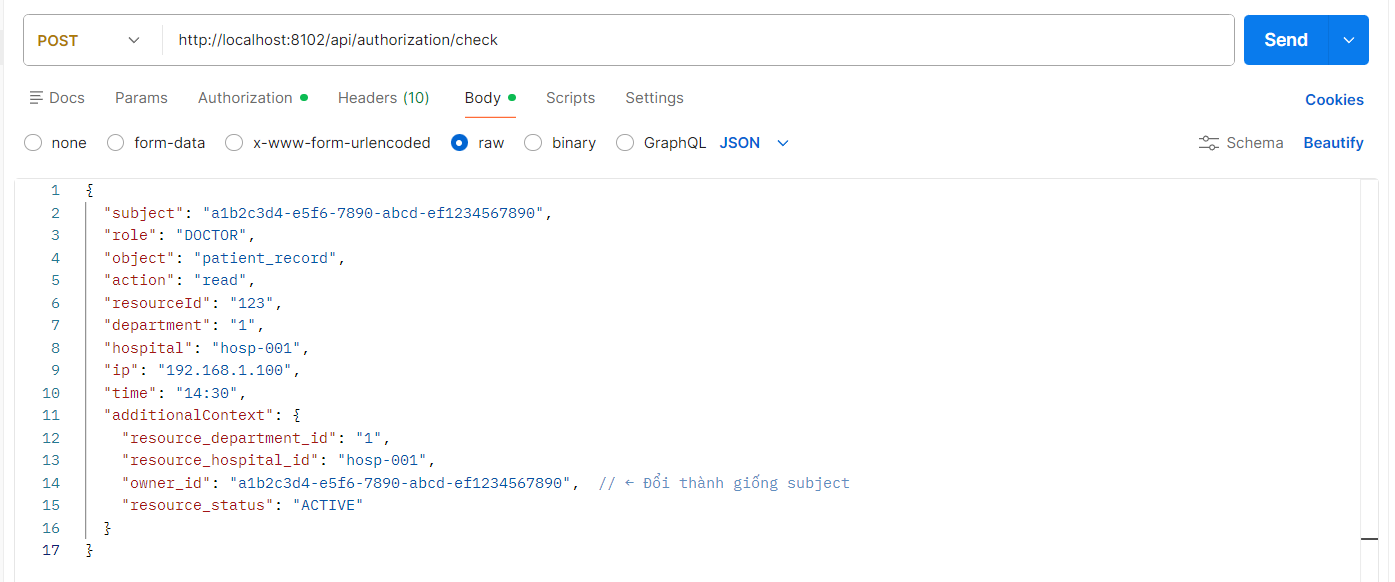
\includegraphics[width=1\linewidth]{images/request.png}
    \caption{Decision Request - Doctor reads patient record}
    \label{fig:request}
\end{figure}


The PDP returns a response that the gateway can enforce immediately. The response includes the final decision and may include a reason and the matched policy identifier for debugging and auditing. Figure~4.2 shows an example response.

\begin{figure}[H]
    \centering
    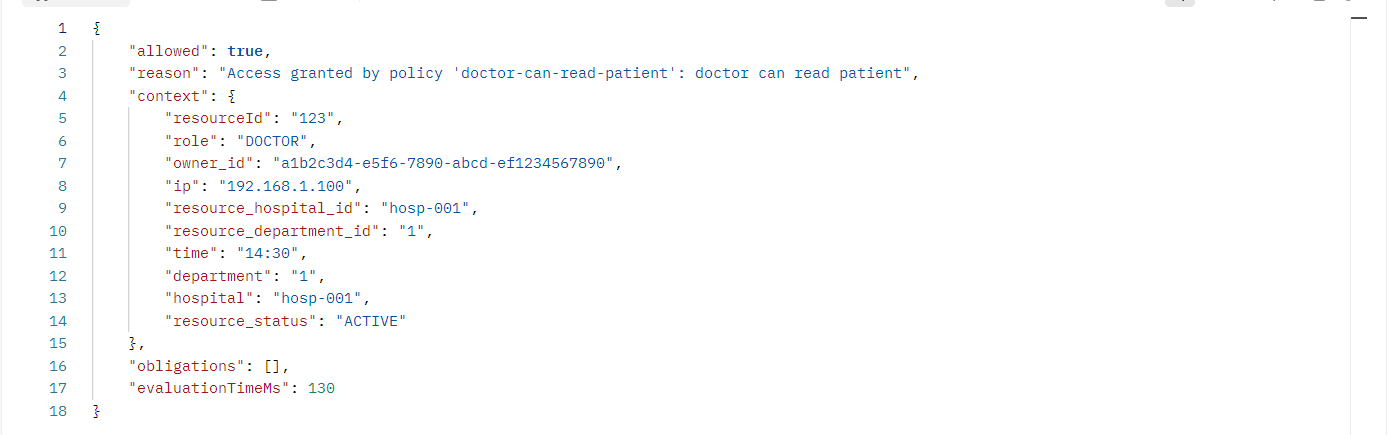
\includegraphics[width=1\linewidth]{images/response.png}
    \caption{Decision Response - Doctor reads patient record}
    \label{fig:response}
\end{figure}


\subsection{Role-centric RBAC–ABAC evaluation logic}
The PDP evaluates access in two steps. First, it checks whether the user's role grants the requested action on the resource type (RBAC baseline). Second, it evaluates attribute-based constraints (ABAC) to narrow access based on context and resource attributes. A request is permitted only if both steps succeed.
\vspace{0.5cm}


The baseline RBAC check prevents policies from granting access outside the role definition. In other words, attributes in this design are used to restrict access, not to expand it beyond the RBAC permission set.
\begin{figure}[H]
    \centering
    \small
    \begin{lstlisting}]
function decide(req):
    assert req.action, req.subject, req.object

  # Step 1: RBAC baseline (role -> permission)
  if not rbac_allows(req.subject.roles, req.action, req.object):
    return DENY("RBAC baseline denied")

  # Step 2: attribute enrichment (PIP)
  attrs = pip_get_attributes(req.subject.keycloak_user_id, req.object, req.resourceId)

  # Step 3: ABAC constraints (OPA)
  opa_input = build_opa_input(req, attrs)  # maps to input.resource.object/action for Rego
  if not opa_allows(opa_input):
    return DENY("ABAC constraints denied")

  return PERMIT("RBAC+ABAC passed")
\end{lstlisting}
    \caption{PDP evaluation flow (pseudo-code)}
    \label{lsting:pseudo-code}
\end{figure}


\subsection{ Attribute retrieval via PIP}
JWT claims provide only basic identity information. Many hospital decisions require extra attributes, such as department, assignment, or patient context. For this reason, the PDP retrieves additional attributes using the Attribute Provider (PIP).

In the application, the PIP collects attributes from two sources:

\begin{itemize}
  \item \textbf{Staff attributes:} obtained from the User Service (e.g., department id, position, staff status).
  \item \textbf{Resource/context attributes:} obtained from domain services such as Patient and Appointment (e.g. sensitivity level, owner id, department,  hospital id).
\end{itemize}

\begin{figure}[H]
    \centering
    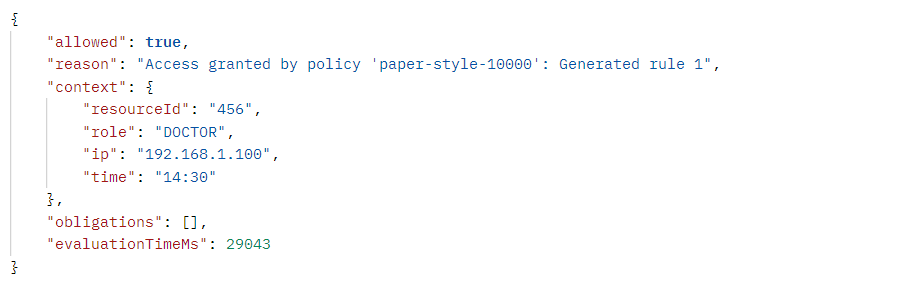
\includegraphics[width=1\linewidth]{images/attributeretrival.png}
    \caption{Attribute Retrieval}
    \label{fig:attributeretrieval}
\end{figure}

The PIP returns a compact attribute bundle. It does not return full business payloads (for example, it does not return the full Patient record content). This reduces data exposure and keeps the PIP focused on decision support.

\subsubsection{Attribute model and attribute selection}
In theory, the HMS exposes many possible attributes at the user, resource, and environment level. However,
not all of them are equally useful for access control. In the hybrid RBAC--ABAC design of this thesis, the
attribute model focuses on a small set of attributes that (i) clearly reduce RBAC over-permission in typical
hospital workflows, (ii) are available and verifiable in the microservices, and (iii) avoid unnecessary
exposure of detailed clinical data.

Conceptually, attributes are organized into three groups:

\begin{itemize}
  \item \textbf{Subject attributes} (user/staff): organizational and employment fields such as
  hospital id, department id, position level, and active status. These refine broad roles (e.g. DOCTOR,
  NURSE) into ``doctor of hospital H, department D, with at least level L, currently active''.

  \item \textbf{Resource attributes} (patient record, appointment, lab order, prescription, etc): context
  about the clinical object, including the resource hospital/department, treatment relationship
  (assigned doctor/owner), and lifecycle status (e.g. appointment status or discharge state). These
  attributes express who the record belongs to and in which department and state it is handled.

  \item \textbf{Environment/context attributes}: dynamic context such as time-of-day and shift
  (working hours flag), network zone (IP range). These attributes capture
  operational constraints such as on-duty access only or internal-network-only access.
\end{itemize}

Table~\ref{tab:attribute-comparison} compares the selected attribute groups with other candidates that
were not used as core attributes in the prototype.

\begin{table}[H]
\centering
\renewcommand{\arraystretch}{1.2}
\begin{tabular}{|p{2.4cm}|p{3.6cm}|p{5.1cm}|p{4.1cm}|}
\hline
\textbf{Category} & \textbf{Core attribute group} & \textbf{Main contribution in HMS} & \textbf{Examples not used as core} \\
\hline
Subject &
Hospital id, department id, position level, active status &
Refine broad roles into concrete staff context (which hospital/department the user works in,
seniority, and whether the staff member is still employed). This directly restricts RBAC permissions
by organization and employment state. &
Age, gender, nationality and other demographic fields; these are rarely the primary criteria for
authorization in common HMS workflows and may raise fairness concerns. \\
\hline
Resource &
Resource hospital/department, assigned doctor/owner, resource status (e.g. ACTIVE, DISCHARGED) &
Encode who the record belongs to, which department handles it, and in which lifecycle state it is.
This allows constraints such as ``only the assigned doctor in the same department may update an
active record''. &
Detailed diagnosis codes, lab result values, and full medical history. These attributes are highly
sensitive, harder to normalize, and more relevant to clinical decision-making than to baseline
authorization decisions. \\
\hline
Environment &
Time/shift (time range, working-hours-only), IP/network zone, ownership flag &
Capture operational context such as on-duty vs off-duty, internal vs external networK. These constraints are common in hospitals and can be enforced without accessing medical
content. &
Fine-grained GPS location, device posture (managed/unmanaged), or behavioural risk scores. These
attributes require additional infrastructure (MDM, tracking, ML) and add complexity that is outside
the scope of this prototype. \\
\hline
\end{tabular}
\caption{Comparison of attribute groups for the hybrid RBAC--ABAC model in the HMS prototype.}
\label{tab:attribute-comparison}
\end{table}

To make the comparison more concrete, the relative contribution of attribute groups can be estimated. In this prototype, resource-level attributes (department, hospital, status, treatment
relationship) are expected to contribute roughly $40\%$ of the ``control value'', subject-level attributes
around $35\%$, and environment/context attributes around $25\%$. Within these groups, four constraints
--- department/hospital matching, treatment relationship, time/shift, and resource status --- jointly
account for about $80$--$85\%$ of the effective reduction of RBAC over-permission, while network act as complementary safeguards.


\subsection{OPA integration and policy input}
\label{sec:opa-integration}

In this prototype, Open Policy Agent (OPA) is used as the policy evaluation engine. The Authorization
Service (PDP) does not hard-code business permissions. Instead, it builds a single input document and
asks OPA to evaluate the current request against the policy set.

\subsubsection{Policy deployment to OPA:}
Policies are managed in the Policy Service (PAP). When a policy is created or updated, the service
transforms the policy rules into an OPA-friendly format and publishes them to OPA as data. In the
normalized format, each rule becomes one entry in \texttt{data.dynamic\_policies}. For multi-rule
policies, the key format is \texttt{\{policyId\}\_\_\{ruleId\}} so OPA can evaluate rules individually
while still knowing their parent policy through fields such as \texttt{parent\_policy\_id} and
\texttt{combining\_algorithm}. This keeps the policy model readable in the Policy UI while making
evaluation in OPA straightforward.

\subsubsection{OPA input structure (request side):}
For each protected request, the PDP builds an OPA input map with three main parts:
\texttt{user}, \texttt{resource}, and \texttt{context}. The \texttt{user} object carries RBAC identity
(role) and subject attributes (e.g., department and hospital). The \texttt{resource} object describes
the target resource (object/type, action, resourceId) and resource-related attributes (e.g., resource
department, hospital, sensitivity, status). The \texttt{context} object contains environment data such as
time-of-day and client IP.
\vspace{0.5cm}


After OPA receives this input, it evaluates the request in a clear order. First, it matches rules by the basic target
fields (\texttt{resource.object} and \texttt{resource.action}) together with subject conditions such as the user's role.
Then it checks the ABAC constraints attached to each matched rule, for example department/hospital matching, ownership,
resource status, time window, and IP range. When more than one rule matches, OPA applies the policy’s combining behavior
and rule priority to decide which result takes effect. In this prototype, a matching Deny rule takes precedence over Allow,
so a deny rule can block access even if another rule allows it. Finally, OPA returns one decision object with
\texttt{allowed} and a short \texttt{reason} string, which is useful for debugging and for audit review.
\vspace{0.5cm}

Before building the final input, the PDP enriches missing fields through the PIP. For example, user
department/hospital is obtained from the User Service, while resource attributes (department/hospital,
sensitivity, status, owner) are obtained from the relevant domain service when a resourceId is present.
This enrichment step returns only the attributes needed for authorization, not full business payloads.

\subsubsection{Calling OPA and mapping the result:}
After the input document is built, the PDP calls OPA using the HTTP API endpoint
\texttt{/v1/data/hospital /authz/allow}. The Rego package \texttt{hospital.authz} returns a single
decision object with fields \texttt{allowed} (true/false), \texttt{reason}, and optional \texttt{obligations}.
The PDP converts this decision into the response format used by the gateway, which then enforces the
final Permit/Deny result. The same decision (including the reason) is also sent to the audit layer so
administrators can review why a request was allowed or denied.
\vspace{0.5cm}



\begin{figure}[H]
    \begin{lstlisting}
        # One decision
default decision := {"allowed": false, "reason": "No matching authorization policy", "obligations": []}

# Highest priority: Patient read own record (GET /api/patients/me) — no constraint check
decision := {"allowed": true, "reason": "Access granted: Patient can read own record (me)", "obligations": []} if {
    "PATIENT" in effective_roles
    input.resource.object == "patient_record"
    input.resource.action == "read"
    no_resource_id
}

else := {
    "allowed": false,
    "reason": sprintf("Access denied by policy '%s' (rule '%s'): %s", [
        display_policy_id(deny_hit[winner_deny_id]),
        winner_deny_id,
        deny_hit[winner_deny_id].policy_name,
    ]),
    "obligations": [],
} if { winner_deny_id }

else := {
    "allowed": true,
    "reason": sprintf("Access granted by policy '%s': %s", [
        display_policy_id(allow_hit[winner_allow_id]),
        allow_hit[winner_allow_id].policy_name,
    ]),
    "obligations": get_obligations(allow_hit[winner_allow_id]),
} if { winner_allow_id }

# -----------------------------------------------------------------------------
# 7. OUTPUT (single element set for authorization-service /v1/data/.../allow)
# -----------------------------------------------------------------------------
allow contains decision if { decision }
    \end{lstlisting}
    \caption{Calling OPA and mapping the result}
    \label{fig:opa-decision-output}
\end{figure}



Listing~\ref{fig:opa-decision-output} shows the final output rule in the \texttt{hospital.authz} package. OPA returns a decision object with three fields: \texttt{allowed}, \texttt{reason}, and \texttt{obligations}. The Authorization Service reads the first element returned from the \texttt{/v1/data/hospital/authz/allow} endpoint and maps it to the API response that the gateway can enforce.


\section{PEP at the Gateway and Request Routing}
\label{sec:gateway_pep}

In the prototype, the API gateway is the main Policy Enforcement Point (PEP). This means every external request must pass
through the gateway before it can reach any business microservice. The gateway has a clear responsibility: it does not
decide whether a request should be allowed, but it \textit{enforces} the decision returned by the PDP. This separation is
important for two reasons. First, it prevents accidental bypass, because domain services are not exposed directly to the
public network. Second, it ensures that all services follow the same enforcement logic, instead of re-implementing access
checks in each microservice.

\vspace{0.5cm}

From an implementation view, the gateway performs three steps on protected endpoints. It validates the JWT token, it
creates a decision request and calls the PDP, and it routes the request only when the outcome is Permit. If the outcome is
Deny, the gateway stops the request early and returns \texttt{403 Forbidden}. The following subsections describe these
steps in detail.

\subsection{JWT validation and claim extraction}
\label{subsec:gateway_jwt}

For each incoming request, the gateway first checks the \texttt{Authorization} header. If the header is missing, or the
token cannot be verified, the gateway returns \texttt{401 Unauthorized}. In the prototype, authentication is delegated to
Keycloak, so the gateway validates the token signature and standard fields such as issuer, audience, and expiration time.

\vspace{0.5cm}


When the token is valid, the gateway extracts a minimal set of claims that are required to build an authorization request.
This typically includes the subject identifier (user id), the role list, and optional tenant fields if they exist in the
token (for example hospital id). These fields are treated as baseline identity context, not as a complete attribute set.
The gateway does not attempt to fetch complex attributes such as department assignment or patient relationship. Those
attributes are collected later by the PDP through the PIP when required by policy constraints.

\vspace{0.5cm}


To support traceability, the gateway can generate or forward a correlation id for each request. This id is included in
logs and can be passed to the PDP and Audit Service. It helps connect a user request with its authorization decision and
domain-service execution.

\subsection{Protected endpoint interception}
\label{subsec:gateway_protected}

Not all endpoints require authorization checks. The gateway therefore distinguishes between public routes and protected
routes. Public routes include endpoints such as health checks or login-related callbacks. Protected routes include HMS
operations that access sensitive resources, such as patient records, appointments, lab results, prescriptions, and billing
data.
\vspace{0.5cm}


For protected routes, the gateway performs authorization before forwarding traffic. The core idea is simple: the gateway
does not call a business service until it receives a Permit decision. This reduces the risk of information leakage. It
also simplifies the domain services, because they can focus on business logic and assume that requests reaching them have
already passed a centralized access check.
\vspace{0.5cm}


In practice, the gateway needs a consistent way to translate an HTTP request into authorization terms. The prototype uses a
mapping from \texttt{(HTTP method, path pattern)} to \texttt{(resource type, action)}. This mapping is important because it
keeps policy writing stable. For example, reading a patient record is always evaluated as \texttt{patient\_record/read}
even if the actual URL contains many path parameters. Similarly, creating an appointment is always evaluated as
\texttt{appointment/create}. This mapping layer makes policies easier to review and reduces ambiguity.

\subsection{Decision request creation and PDP call}
\label{subsec:gateway_pdp_call}

Once the gateway confirms that a request targets a protected endpoint, it creates a decision request and calls the PDP.
The decision request is designed to be compact and consistent across all services. It contains four logical parts:
\texttt{subject}, \texttt{action}, \texttt{resource}, and \texttt{context}.
\vspace{0.5cm}


The \texttt{subject} is built from JWT claims. It includes the user identifier and the user roles. The \texttt{action} and
\texttt{resource} are built from the gateway mapping described earlier. The gateway also extracts a resource id when it is
available in the path, for example \texttt{/patients/\{patientId\}}. The \texttt{context} contains runtime metadata that can
be useful for constraints, such as request time and client IP address. The gateway keeps this context minimal and avoids
sending unnecessary user or business information to the PDP.
\vspace{0.5cm}


After building the decision request, the gateway calls the Authorization Service. If the PDP returns Permit, the gateway
routes the original request to the target microservice and returns the service response to the client. If the PDP returns
Deny, the gateway returns \texttt{403 Forbidden} and does not call the domain service. This behavior makes enforcement
explicit and consistent for all protected endpoints.
\vspace{0.5cm}


The prototype also needs a clear strategy when the PDP is unavailable. In a hospital setting, sensitive data access should
not be granted when the decision service is down. For this reason, the recommended default for protected endpoints is
\textit{fail-close}. In fail-close mode, the gateway denies the request when it cannot obtain a decision within a timeout.
The gateway logs the failure with the correlation id so that the event can be investigated. Non-sensitive routes can use a
different handling strategy if needed, but protected data access should remain conservative.
\vspace{0.5cm}


Overall, the gateway implementation provides a single enforcement point for the HMS. It ensures that authorization is
checked before any business service is reached, and it keeps routing behavior aligned with the role-centric hybrid policy
model evaluated by the PDP.
\section{User Interface}
The implementation includes a simple web UI to demonstrate end-to-end workflows. The UI is designed to reflect
different roles and their typical tasks. It does not contain authorization logic. It only displays available actions
and sends requests to the gateway. The final decision is always enforced at the gateway and PDP.


\subsection{Role-based layout and menu}
The application uses one shared layout for authenticated users and different default dashboards per role. The role comes from the session (Keycloak \texttt{realm\_access.roles} or a mapped claim). A mapping in the frontend (\texttt{DASHBOARD\_BY\_ROLE}) defines the default path for each role: admin $\to$ \texttt{/admin}, doctor $\to$ \texttt{/doctor}, nurse $\to$ \texttt{/nurse}, patient $\to$ \texttt{/patient}, pharmacist $\to$ \texttt{/pharmacist}, and so on. The sidebar menu (\texttt{Menu.tsx}) uses a \texttt{useRole} hook to read the current role and shows only items whose \texttt{visible} list includes that role. So patients see appointments and their own data; doctors and nurses see patients, appointments, lab orders, and related lists; pharmacists see prescriptions and medicines; admins see everything plus policy management and audit logs; external auditors see only the audit log page. Hiding a menu item is only for convenience; the gateway and PDP enforce access. If a user opens a URL they are not allowed to use, the API returns 403 and the UI shows an error. Table~\ref{tab:role-ui} summarises the main screens per role.

\begin{table}[H]
\centering
\begin{tabular}{|l|l|}
\hline
\textbf{Role} & \textbf{Main screens / functions} \\
\hline
Admin & Dashboard, employees, patients, appointments, lab, prescriptions, policies, audit logs \\
\hline
Doctor & Patients, appointments, lab orders/results, prescriptions (view) \\
\hline
Nurse & Patients, appointments, lab orders/results, prescriptions (view) \\
\hline
Receptionist & Appointments, scheduling, patients (limited) \\
\hline
Patient & My appointments, prescriptions, lab results \\
\hline
Lab Tech & Lab orders, lab results \\
\hline
Pharmacist & Prescriptions, medicines, inventory \\
\hline
Billing Clerk & Appointments, billing, invoices \\
\hline
External Auditor & Audit logs (read-only) \\
\hline
\end{tabular}
\caption{Main UI entry points and functions by role.}
\label{tab:role-ui}
\end{table}

\begin{figure}[H]
    \centering
    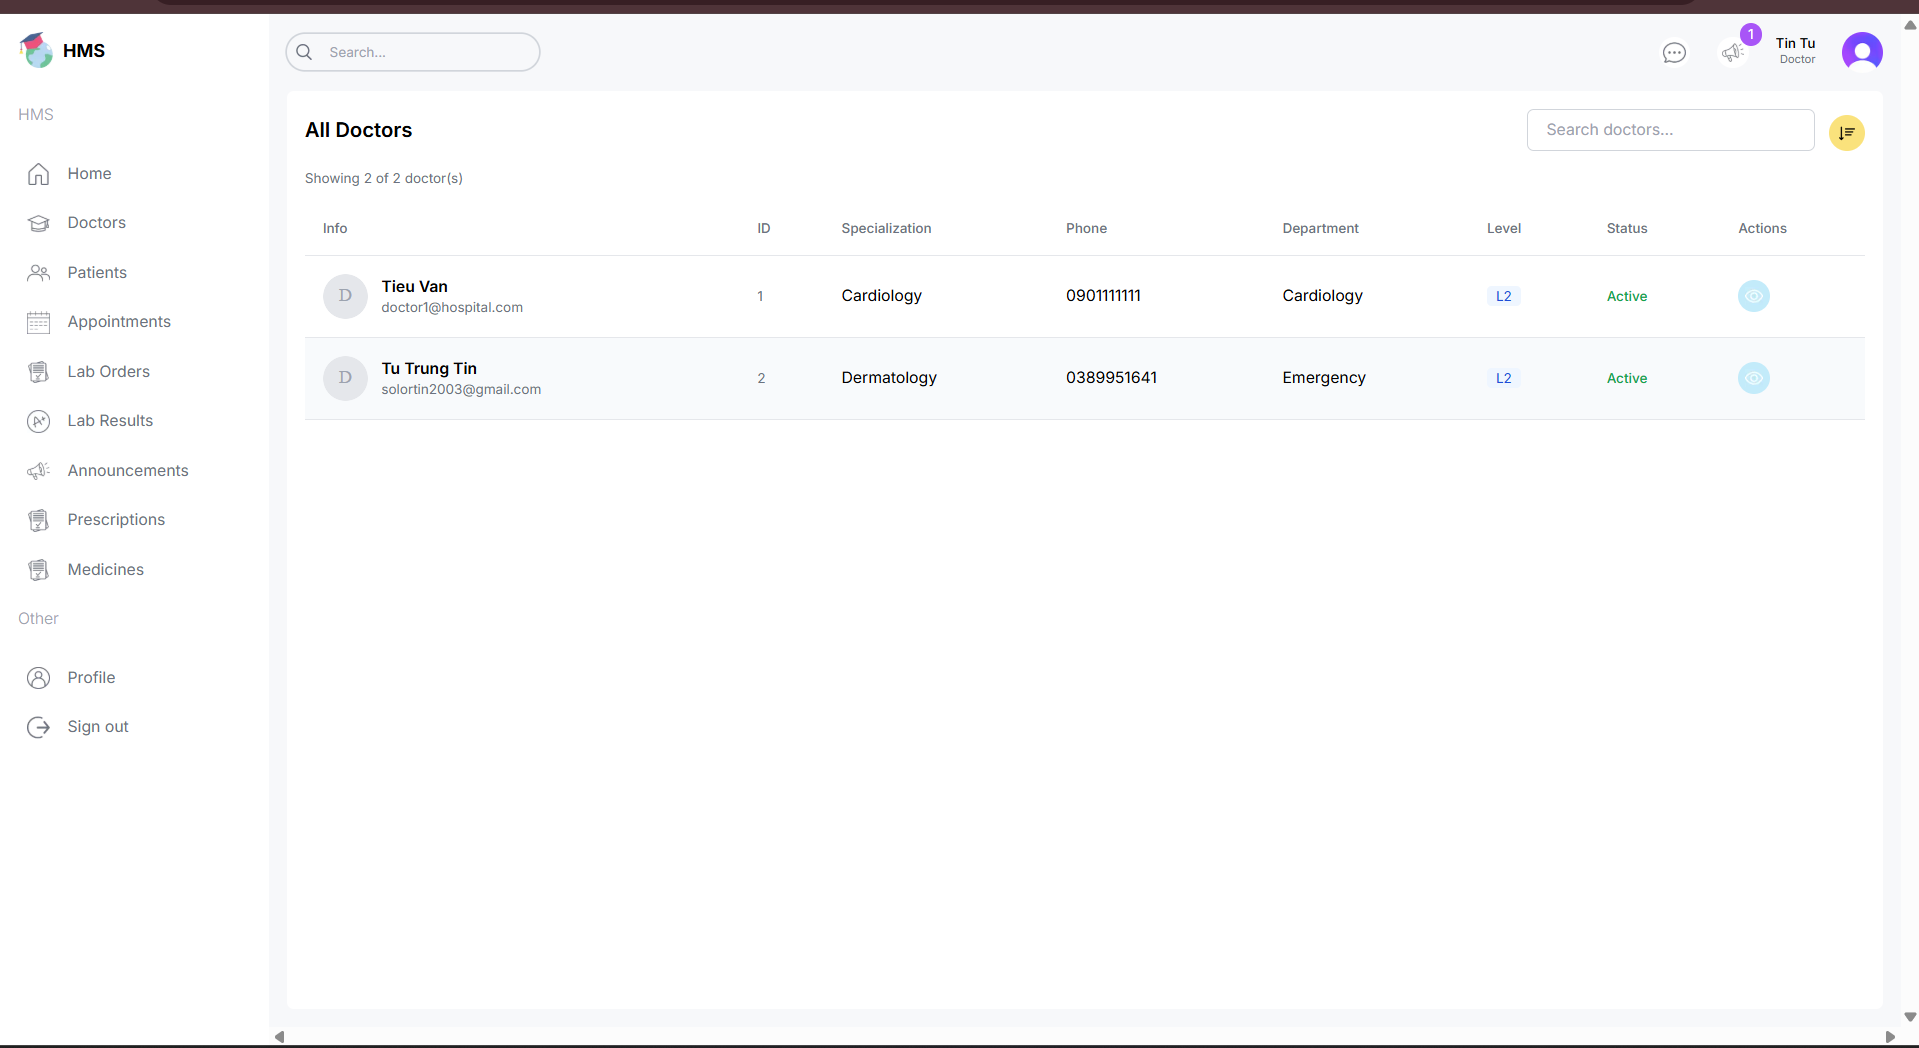
\includegraphics[width=0.75\linewidth]{images/doctorpage.png}
    \caption{Main UI for doctor role}
    \label{fig:doctorui}
\end{figure}


\begin{figure}[H]
    \centering
    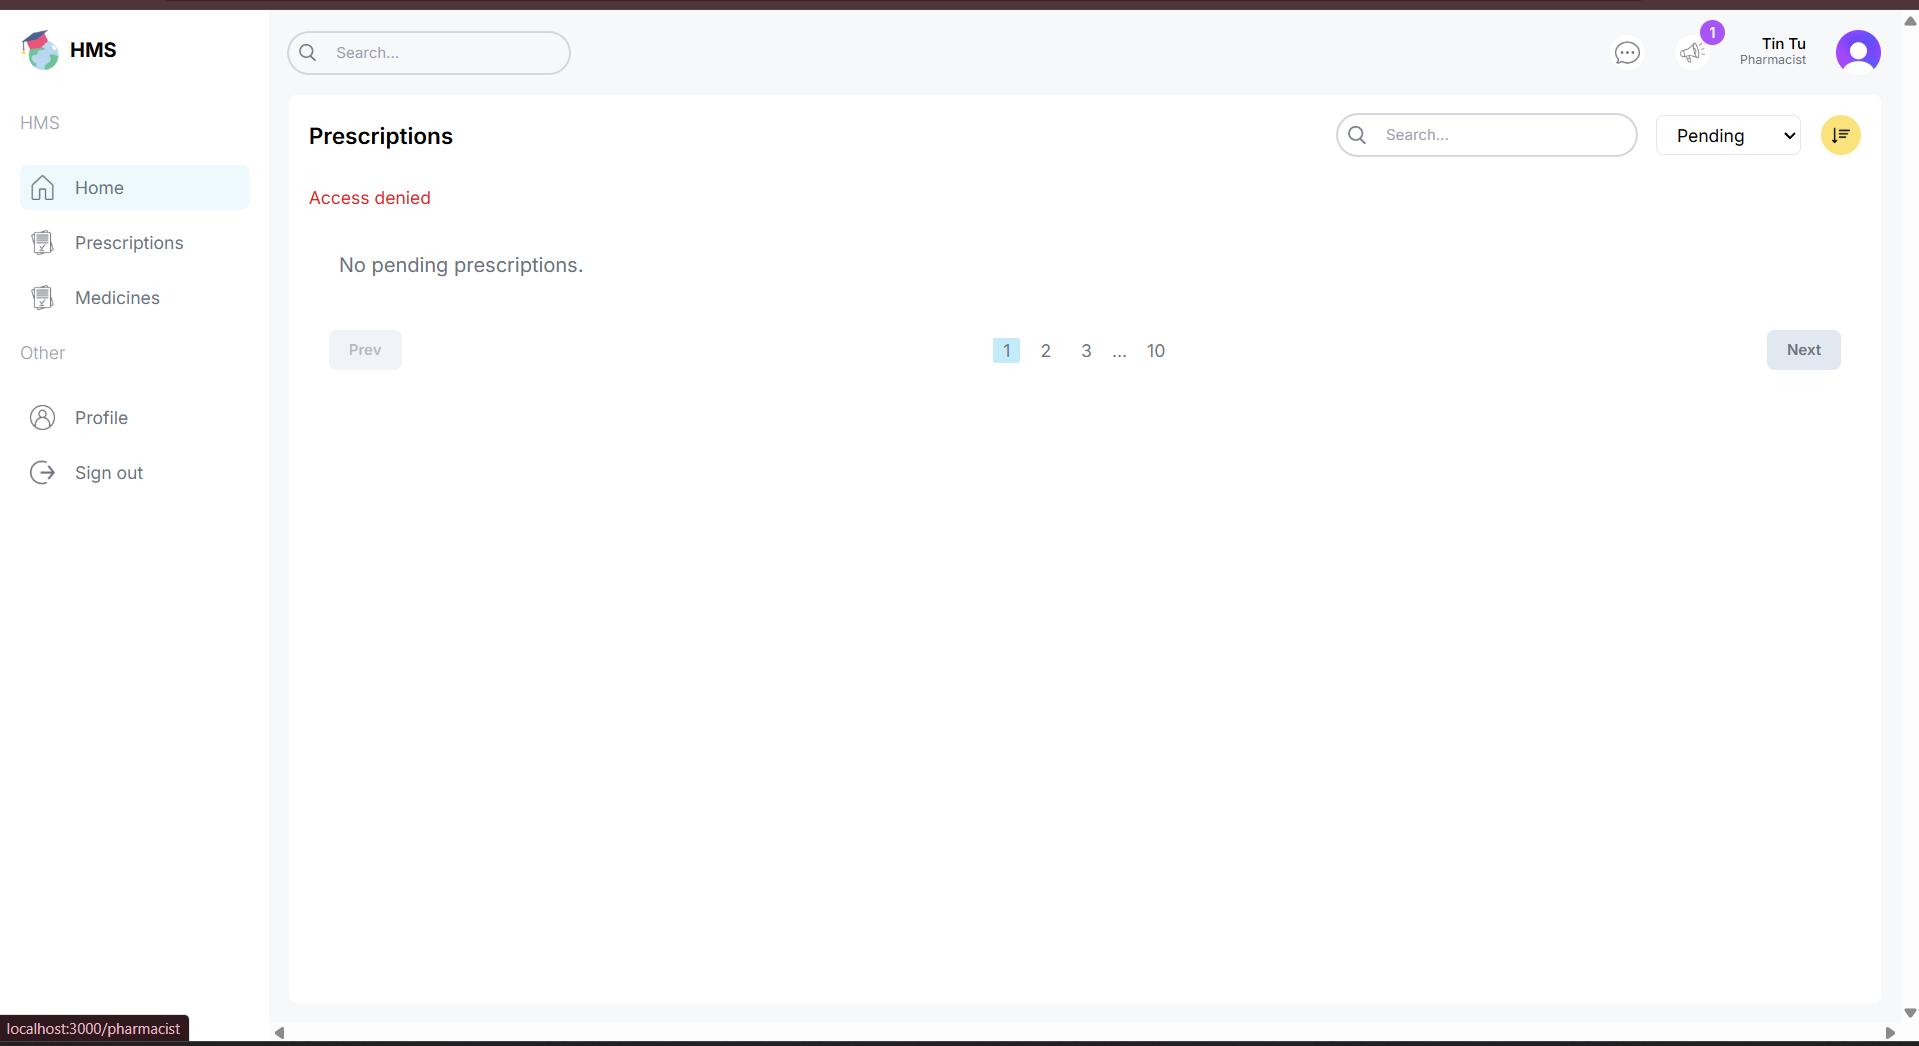
\includegraphics[width=0.75\linewidth]{images/pharmacistui.png}
    \caption{Main UI for pharmacist role}
    \label{fig:pharmacistui}
\end{figure}


\subsection{Policy Management Page}
Policy management is provided for the admin role. The goal of this UI part is to make policy operations transparent:
an admin can view existing policies, inspect the rule content, and create a new policy in a controlled format. 
\vspace{0.5cm}


Figure~\ref{fig:policymanagement} shows the policy list screen. This screen displays the policy name, status, and basic metadata so that an admin can quickly find the correct policy. From this list, the admin can open a policy to see its full content.
\begin{figure}[H]
    \centering
    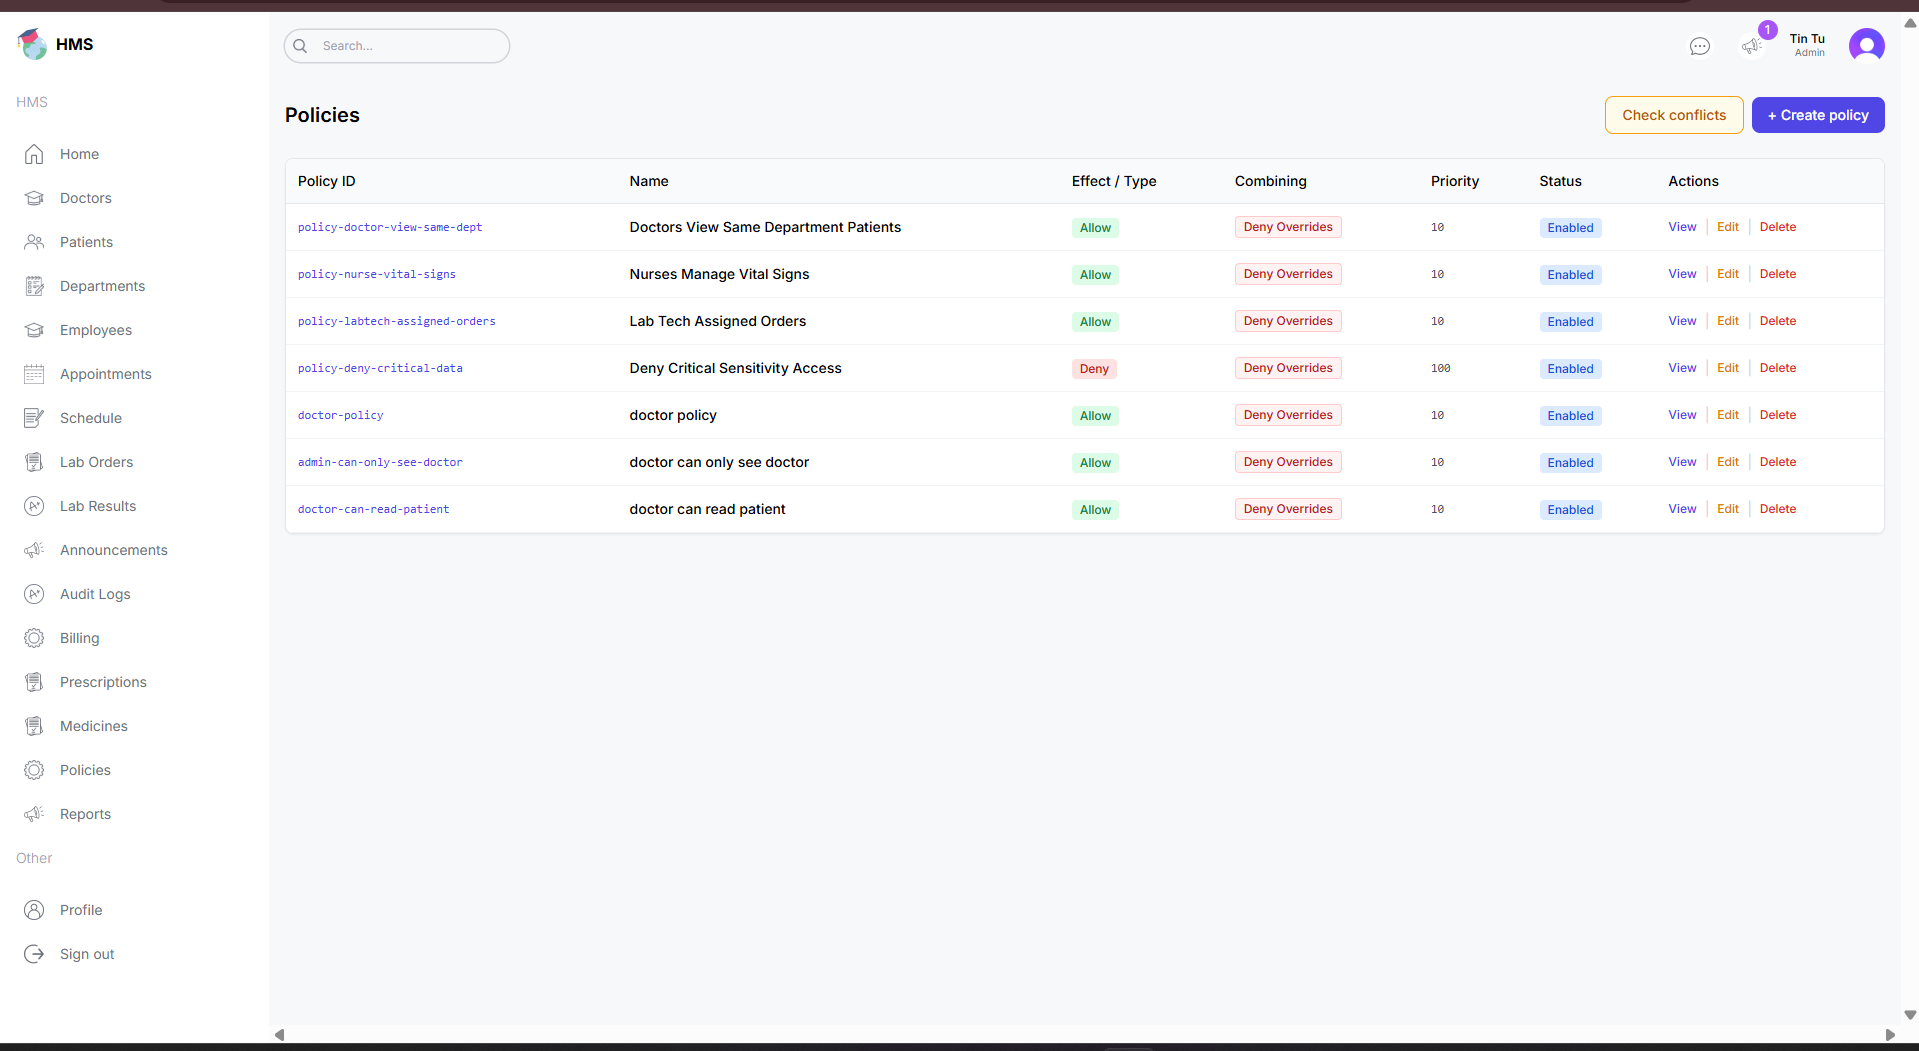
\includegraphics[width=1\linewidth]{images/policymanagement.png}
    \caption{Policy Management Page}
    \label{fig:policymanagement}
\end{figure}

Figure~\ref{fig:policydetail2} shows the policy detail screen. This view is important for review and debugging. It allows the admin to verify the target roles, resource type/object, allowed actions, effect (Allow/Deny), priority, and constraints (such as time range
or department rules). In the role-centric hybrid design of this thesis, roles define baseline access, while attributes are
mainly used as constraints to narrow access in specific contexts. This is reflected in the policy detail view, where the
role and action/resource fields are always explicit, and constraints are shown as structured conditions.

\begin{figure}[H]
    \centering
    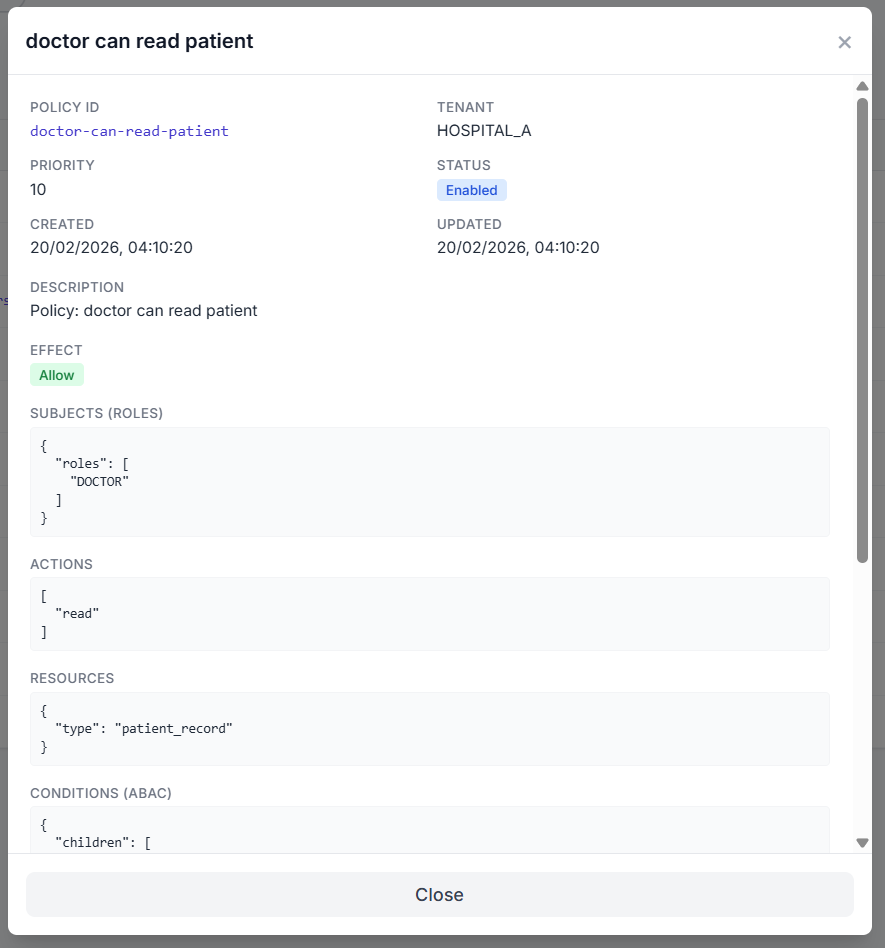
\includegraphics[width=0.65\linewidth]{images/policydetail.png}
    \label{fig:policydetail}
\end{figure}


\begin{figure}[H]
    \centering
    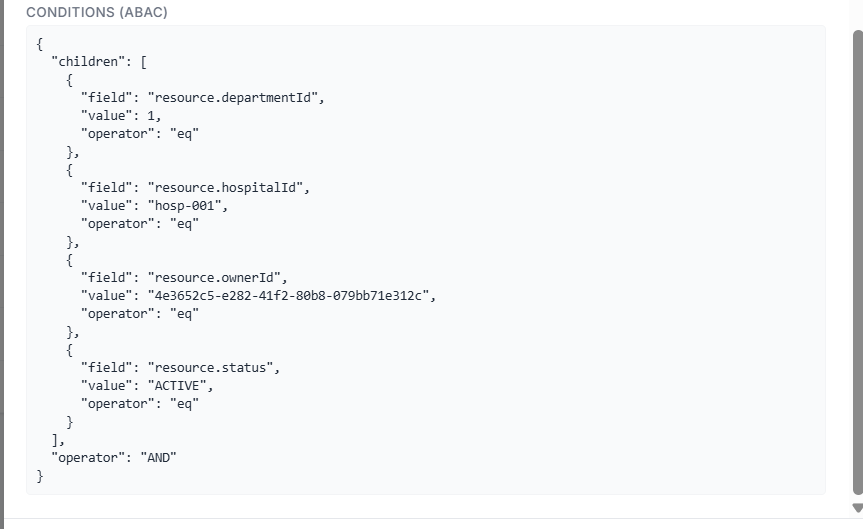
\includegraphics[width=0.65\linewidth]{images/policydetail2.png}
    \caption{Policy Detail Page}
    \label{fig:policydetail2}
\end{figure}

Figure~\ref{fig:policycreate} shows the policy creation screen. This screen is used to add a new policy or rule. In the prototype, the form is designed to reduce input errors. Fields such as action names and resource types follow a fixed naming convention so that
policies remain consistent across services. After a new policy is created, it is stored in the Policy Service database and
then published to OPA. This keeps policy authoring separate from policy evaluation.


\begin{figure}[H]
    \centering
    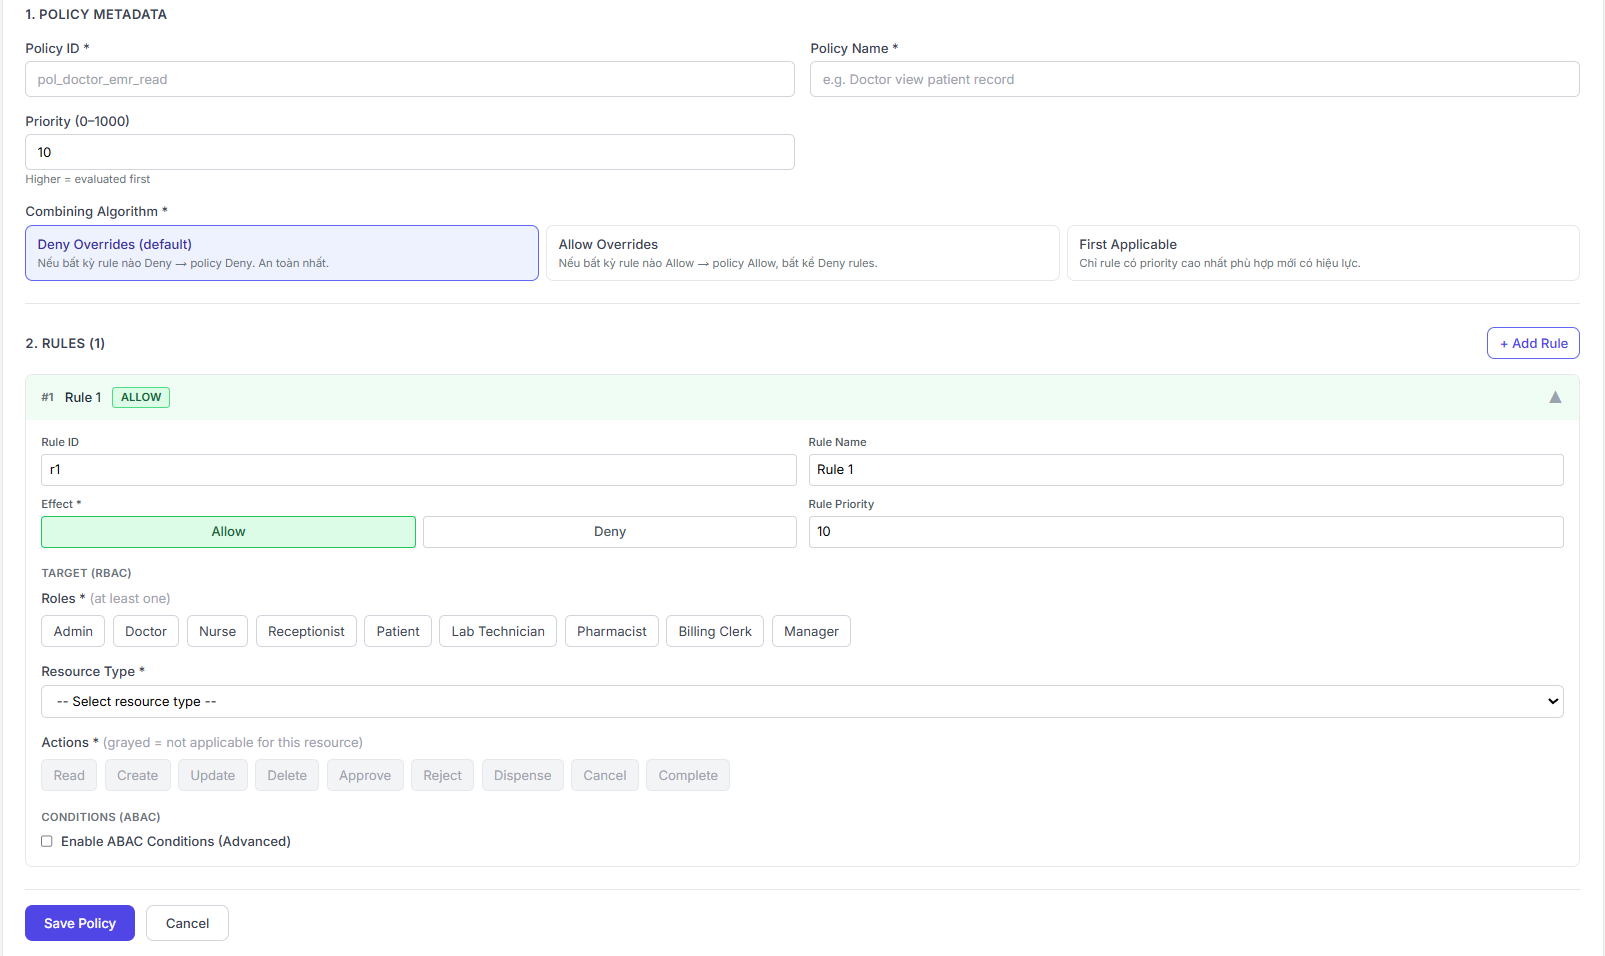
\includegraphics[width=1\linewidth]{images/polcreate.png}
    \caption{Policy create Page}
    \label{fig:policycreate}
\end{figure}





\subsection{Audit logs Page}
Audit logs are required in a hospital setting because medical data is sensitive and access must be traceable. The prototype
includes audit screens so that administrators (or authorized auditors) can review access activities and investigate abnormal
events.
\vspace{0.5cm}


Figure~\ref{fig:auditlogs} shows the audit log list screen. It provides a searchable overview of access events. A typical log entry includes the timestamp, subject identifier, role, action, resource type/object (or resource id), and the final decision (Permit/Deny).
This list view is useful for quick monitoring and for locating suspicious requests.
\begin{figure}[H]
    \centering
    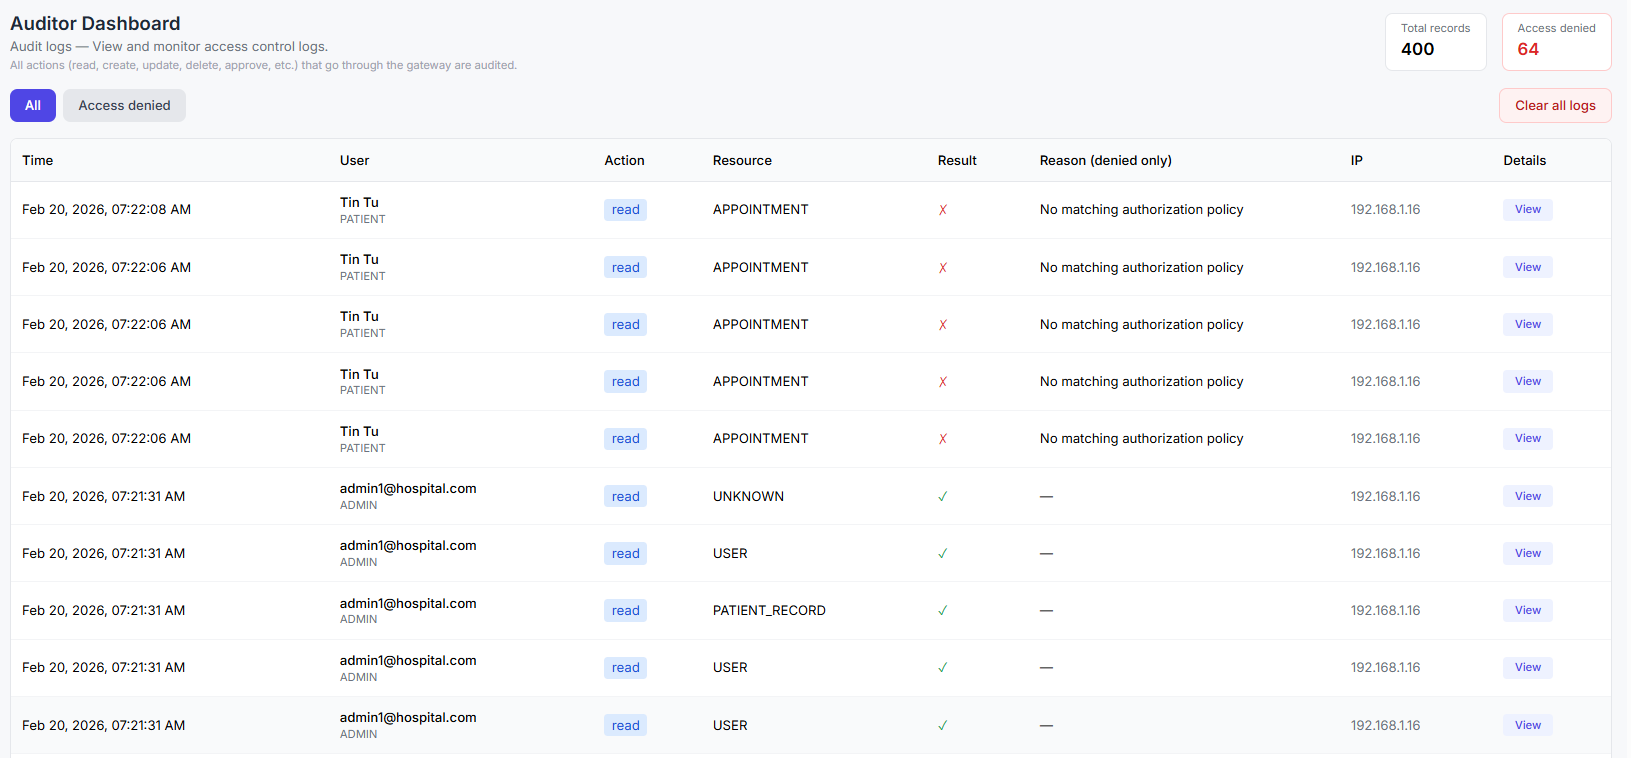
\includegraphics[width=1\linewidth]{images/auditlogs.png}
    \caption{Audit logs Page}
    \label{fig:auditlogs}
\end{figure}
Figure~\ref{fig:auditlogsdetail} shows the audit log detail screen. This screen provides more context for a specific event, such as request metadata and which policy (or rule) matched the request. This detail view is helpful when validating the correctness of policies during testing. It is also useful in real operation to support incident investigation and compliance requirements.
\begin{figure}[H]
    \centering
    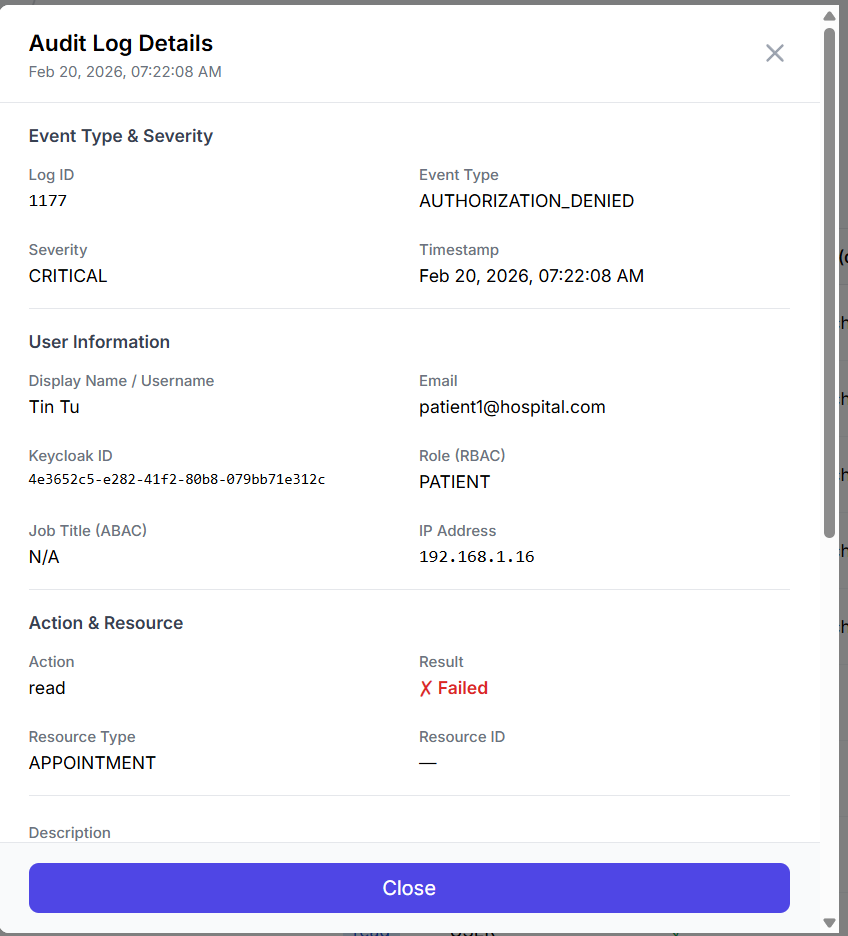
\includegraphics[width=0.55\linewidth]{images/auditlogdetail.png}
    \caption{Audit logs Detail Page}
    \label{fig:auditlogsdetail}
\end{figure}

Overall, the UI in this application serves two purposes: it demonstrates role-based workflows for HMS functions, and it provides
a practical way to manage policies and review audit trails. The next sections build on these screens to describe how policies
are evaluated and how the system can be tested and validated.

\subsection{Policy-aware navigation and access feedback}
\label{subsec:ui_policy_aware}
The UI is designed to be policy-aware at the navigation level, mainly to improve usability. After login, the UI reads the
user roles from the authentication token and shows the menus that match the role. For example, a doctor sees clinical menus
such as appointments and patient-related views, while an administrator sees policy and audit menus. This behavior reduces confusion for users and helps them focus on relevant workflows.

Hiding menu items is only a usability feature and does not enforce authorization. The final decision is always enforced by
the gateway (PEP) and the authorization layer (PDP/OPA). When a user tries to access an endpoint or page that is not
allowed, the UI provides clear feedback based on HTTP status codes:
\begin{itemize}
  \item \textbf{401 Unauthorized:} the session is missing/expired or the JWT cannot be validated. The UI prompts the user to
  sign in again.
  \item \textbf{403 Forbidden:} the user is authenticated, but the request is denied by policy. The UI shows an access
  denied message and avoids rendering sensitive data.
\end{itemize}
\begin{figure}[H]
    \centering
    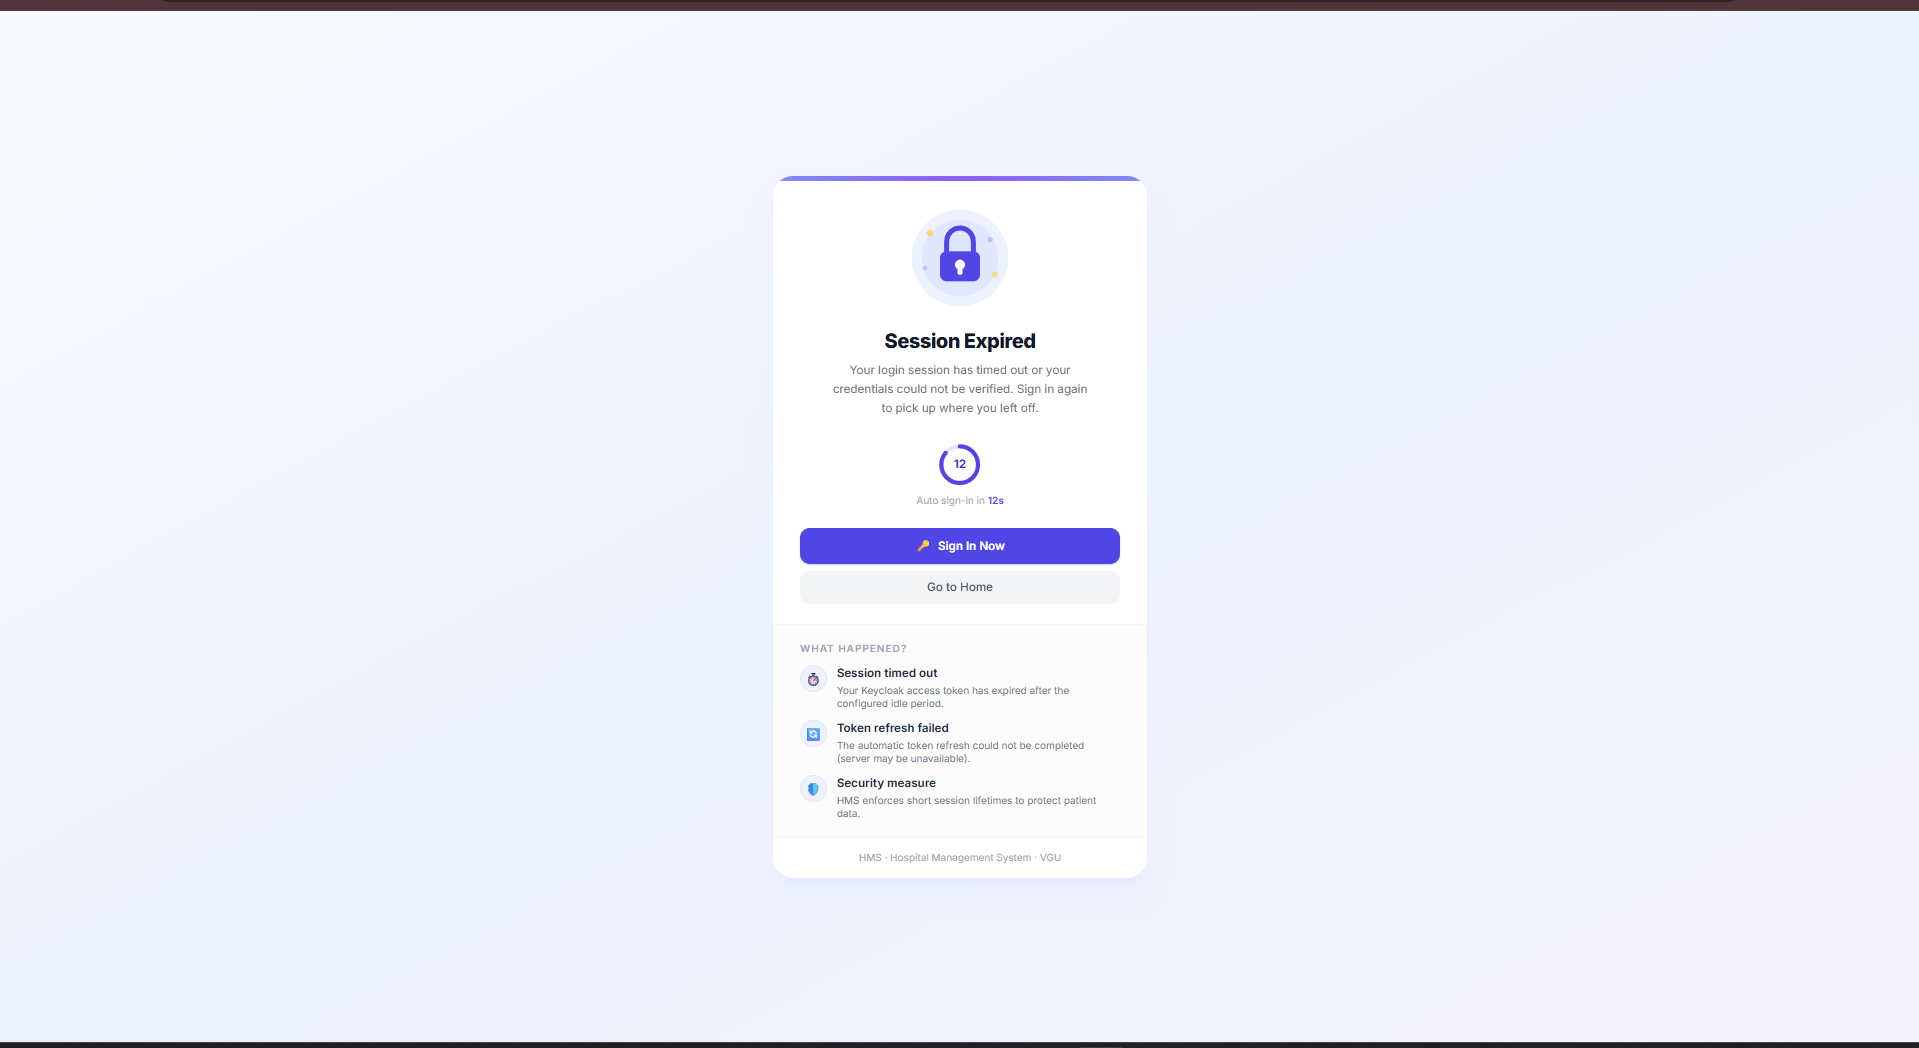
\includegraphics[width=1\linewidth]{images/ui-401-unauthorized.png}
    \caption{Policy-aware access feedback in the UI - Unauthorized, the session is missing/expired (HTTP 401)}
    \label{fig:ui-401-unauthorized}
\end{figure}


\begin{figure}[H]
    \centering
    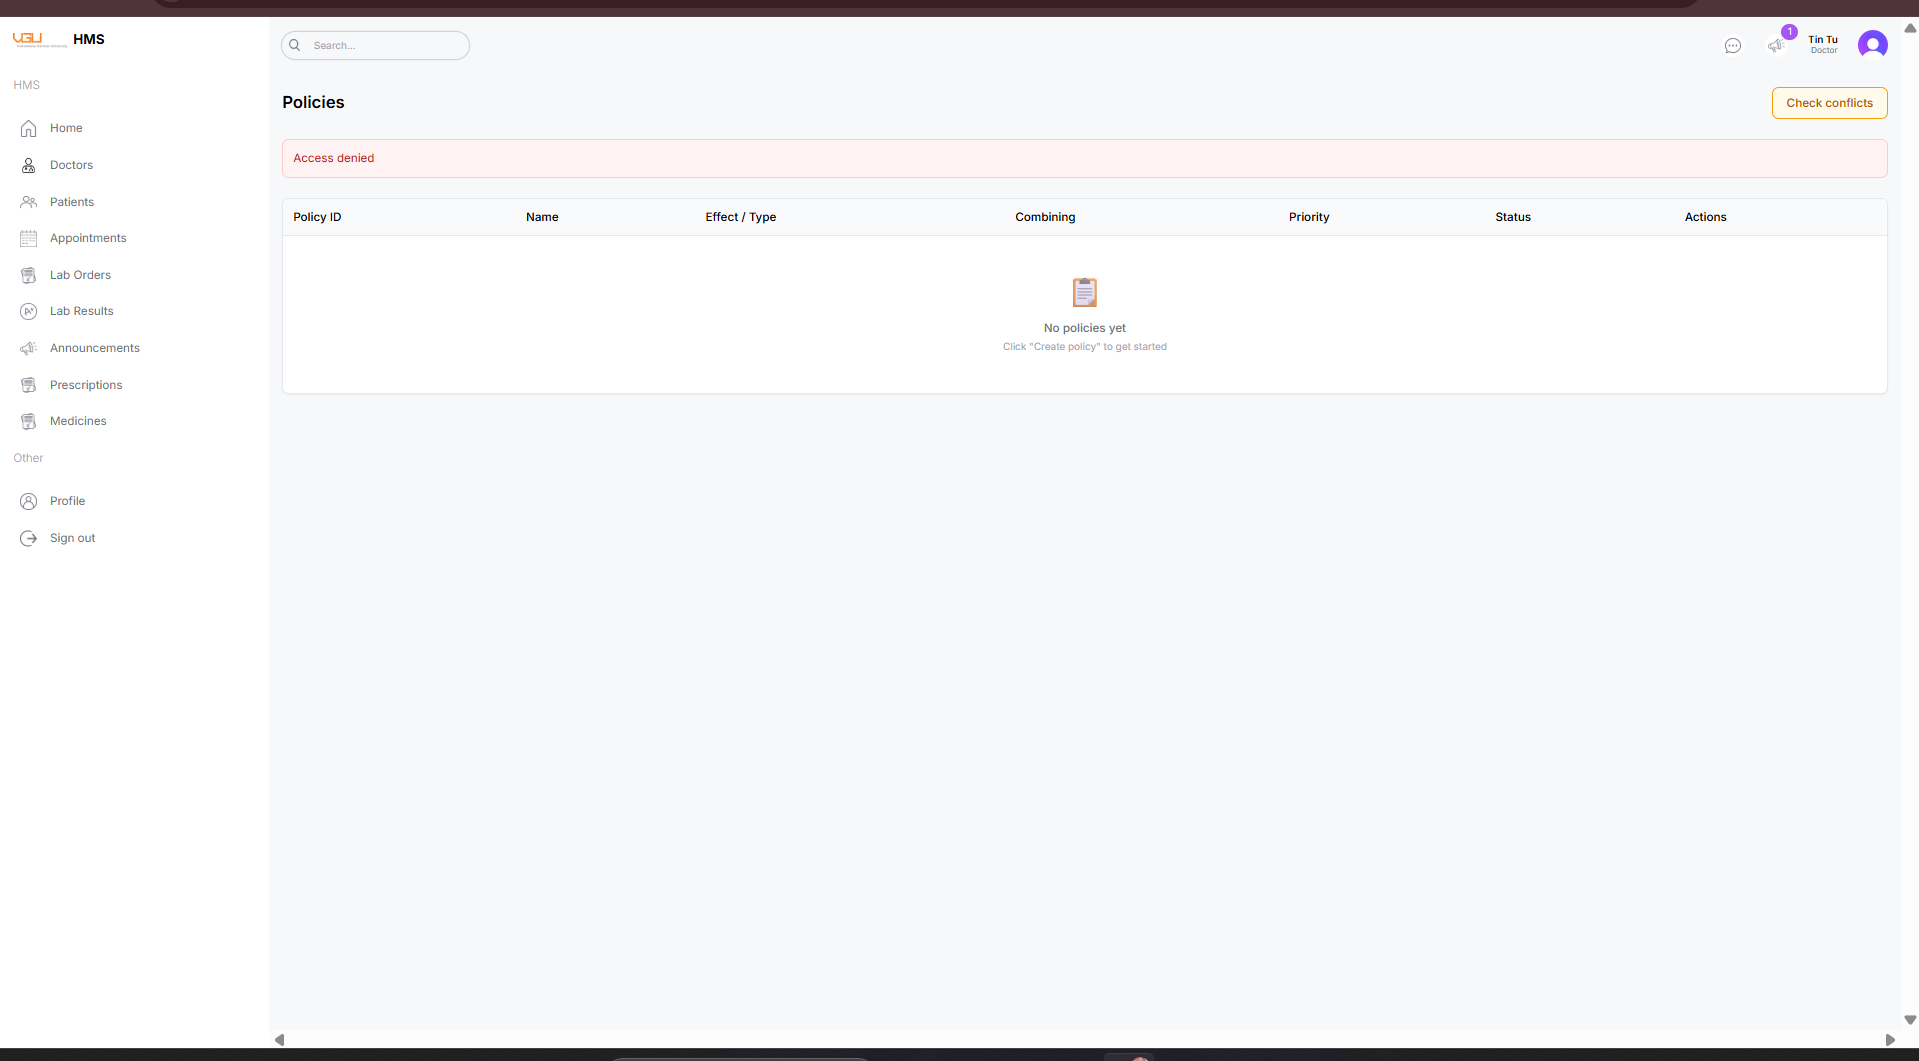
\includegraphics[width=1\linewidth]{images/ui-403-access-denied.png}
    \caption{Policy-aware access feedback in the UI - Authenticated but denied by policy (HTTP 403)}
    \label{fig:ui-403-access-denied}
\end{figure}




\section{Policy Conflict Detection Implementation}
\label{sec:policy-conflict-detection-2}

Policy conflict detection is implemented in the policy service. Its job is to find pairs of rules that can contradict each other or overlap in a way that makes the final decision unclear. The idea follows the design in Section~\ref{sec:policy-conflict-detection}: we do static analysis on the rules stored in the policy service, without running real requests. The result is a list of conflict pairs that the admin can review and fix (e.g. by merging rules, changing effects, or removing one of them).


\subsection{When detection runs and what it returns}

Detection can run in two ways. First, the admin can trigger it from the policy management page: after loading the list of policies, they click ``Check conflicts'' and the frontend calls the gateway, which forwards the request to the policy service. Second, the policy service exposes two REST endpoints. \texttt{GET /api/policies/conflicts} runs detection on all enabled policies and returns a single result. \texttt{POST /api/policies/conflicts/detect} accepts a body \texttt{\{ "policyIds": ["id1", "id2", ...] \}} and runs detection only on those policies. Both endpoints return the same shape: \texttt{totalPolicies} (number of rules considered after expanding each policy into its rules), \texttt{conflictCount}, \texttt{conflicts} (a list of conflict pairs), and \texttt{detectionTimeMs}. The frontend shows this in a panel: if \texttt{conflictCount} is 0 it shows ``No policy conflicts''; otherwise it lists each pair with the conflict type (e.g.\ \texttt{AUTH\_CONFLICT} or \texttt{REDUNDANCY\_CONFLICT}), the resource type, the overlapping actions, the reason text, and when available a witness (a sample attribute map that matches both rules). Figure~\ref{fig:policyconflitdetection} shows a real run: 11 policies scanned in 36\,ms with one redundancy conflict between \texttt{doctor-policy\_r1} and \texttt{admin-create-patient\_r1} on resource \texttt{patient\_record} for actions read, create, update, with witness \texttt{\{"roles":"ADMIN", "type":"patient\_record"\}}. 


\begin{figure}[H]
    \centering
    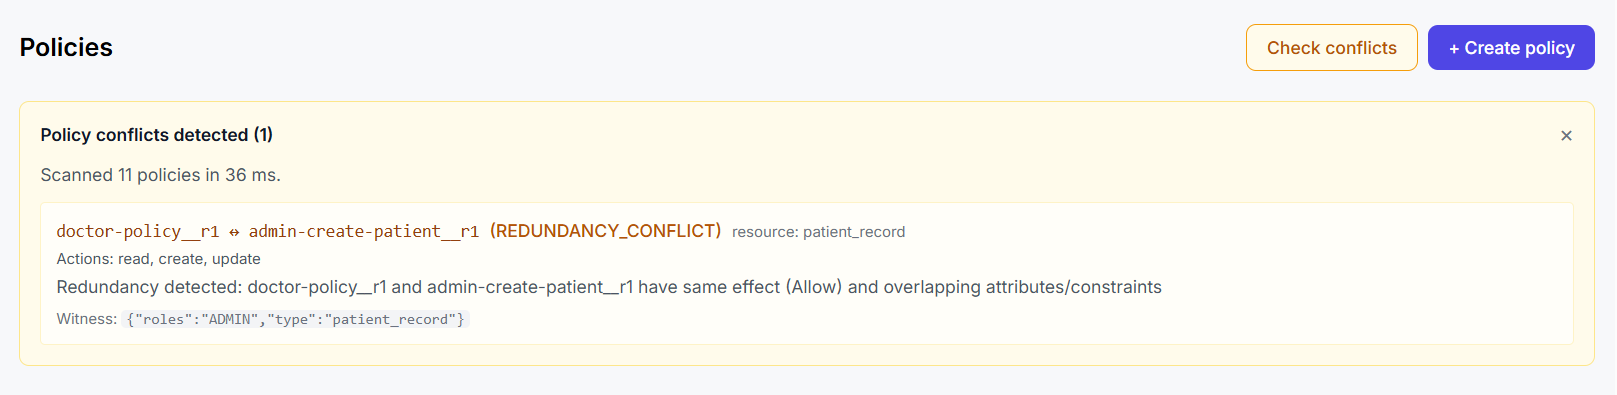
\includegraphics[width=1\linewidth]{images/policyconflict.png}
    \caption{Policy Conflict Detection Result}
    \label{fig:policyconflitdetection}
\end{figure}

\subsection{Types of conflicts}

The implementation detects two kinds of conflicts:
\begin{itemize}
    \item \textbf{Authorization conflict (Allow vs Deny).} Two rules conflict in this sense if one has effect Allow and the other Deny, and there exists at least one request that would match both rules. So we require: (1) the two rules have different effects; (2) their action sets overlap (e.g. both include \texttt{read}); (3) they apply to the same resource type (or one of them does not restrict resource type); (4) for each attribute that both rules use (subject or resource), the value sets intersect (e.g. one says role in \texttt{\{DOCTOR\}} and the other says role in \texttt{\{DOCTOR, NURSE\}}); and (5) if both rules have a time-range constraint, those intervals overlap. When all these hold, we report an \texttt{AUTH\_CONFLICT} and include the overlapping actions and a short reason (e.g. which two policies and that they have conflicting effects for those actions).
    \item \textbf{Redundancy.} Two rules are redundant if they have the same effect (both Allow or both Deny) and again there is some request that matches both. So the conditions are the same as above except the effects must be equal. In that case we report \texttt{REDUNDANCY} (or \texttt{REDUNDANCY\_CONFLICT} in the code). The admin may want to remove one of the rules or merge them to keep the policy set simpler.
\end{itemize}


Each conflict pair in the result includes the two rule identifiers (policy id and rule id), the conflict type, the list of overlapping actions, and a \texttt{reason} string. Optionally a \texttt{witness} (or \texttt{witnessRequest}) is provided: a sample attribute-to-value map that would satisfy both rules, which helps when debugging.

\subsection{How the algorithm works}

The service loads all enabled policies (or only the ones requested in the POST body), then expands each policy into a list of rules. Each rule has subject attributes (e.g. role, department), resource type, actions, and optionally object attributes and conditions (e.g. time range). Rules that have no actions or no subject/resource attributes are skipped; they cannot participate in a conflict in our definition.
\vspace{0.5cm}


To avoid comparing every pair of rules (which would be too slow with many policies), the code does a few things. First, rules are grouped by resource type. Within each group, rules are split into Allow and Deny. Only Allow--Deny pairs need to be checked for authorization conflicts; within the same effect we only check for redundancy. Second, within each resource-type bucket, rules are indexed by action: for each action we keep a list of rule indices. So we only compare an Allow rule and a Deny rule if they share at least one action. That cuts down the number of pairs a lot. Third, for rules that have a time-range constraint, the code builds a list of disjoint time intervals (using \texttt{TimeIntervalReducer}) and uses binary search (\texttt{TimeIntervalBinarySearch}) to find which rules overlap in time. So we do not need to compare every Allow with every Deny when many rules have time constraints; we only compare when the time intervals overlap.
\vspace{0.5cm}


For each candidate pair (Allow, Deny) or (same-effect, same-effect), the code checks attribute overlap. Subject attributes and object (resource) attributes are compared: for each attribute that appears in both rules, we check whether the value sets intersect (e.g. \texttt{\{DOCTOR\}} and \texttt{\{DOCTOR, NURSE\}} intersect). If one rule uses attributes that the other does not have, we still need some overlap on the shared attributes; the exact logic (full overlap vs partial) is what distinguishes conflict types like exception vs association in the literature; here we report either \texttt{AUTH\_CONFLICT} or \texttt{REDUNDANCY} with a reason string.
\vspace{0.5cm}

\subsection{Policy governance and misuse prevention (implementation)}
\label{sec:governance-implementation}
Section~\ref{sec:policy-governance} (Chapter~3) defines governance controls to prevent conflicts and abuse of power in the hybrid system. This subsection describes how they are implemented and demonstrated in the prototype, so that the design is not only stated but \emph{solved} from theory to demo.
\vspace{0.5cm}

\paragraph{Conflict-on-save (enforcing conflict-freedom).}
The policy service is configured with \texttt{policy.conflict-on-save: strict} in the main deployment. On create or update, the service runs conflict detection on the proposed state (all enabled policies plus the new or updated one). If any AUTH\_CONFLICT is found, the save is rejected with HTTP 409 and a conflict report is returned (policy id, rule ids, overlapping actions, reason). The UI displays this report so the administrator can resolve the conflict before retrying. Thus the invariant that the enabled policy set is conflict-free is maintained at every successful save.
\vspace{0.5cm}

\paragraph{Restricted policy administration (enforcing write-restriction).}
Policy write operations (create, update, delete policies; trigger OPA sync; run conflict detection) are protected by \texttt{@PreAuthorize("hasRole('ADMIN')")} in the policy service and by gateway route rules that allow only the ADMIN role for \texttt{/api/policies} write endpoints. A non-admin user who attempts to create or update a policy receives HTTP 403 Forbidden. This enforces the write-restriction invariant and prevents abuse by non-privileged users.
\vspace{0.5cm}

\paragraph{Traceability.}
Each policy record stores \texttt{version}, \texttt{created\_at}, \texttt{updated\_at}, \texttt{created\_by\_keycloak\_id}, and \texttt{updated\_by\_keycloak\_id}. This provides who-changed-what-when for every policy change and supports accountability. Optionally, policy create/update events can be published to the audit service so that privileged operations appear in the audit log; the prototype's audit path already records authorization decisions and can be extended to include policy lifecycle events.
\vspace{0.5cm}

\paragraph{Demo scenarios for governance.}
To show that conflict and abuse are actively prevented, the following scenarios can be demonstrated: (1) \textbf{Conflict prevention:} add or edit a policy so that a new rule conflicts (Allow vs Deny) with an existing rule for the same action and resource; the API returns 409 and the UI shows the conflict report; the policy set is unchanged. (2) \textbf{Abuse prevention:} call the policy create or update endpoint with a user that has a non-admin role (e.g.\ DOCTOR); the gateway or policy service returns 403. (3) \textbf{Traceability:} after an admin updates a policy, inspect the policy record or audit log to see the new version, timestamp, and \texttt{updated\_by} identity. These scenarios link Section~\ref{sec:policy-governance} to the running system and show that the hybrid implementation is effectively controlled.
\vspace{0.5cm}

\section{Evaluation}
\label{sec:evaluation}

This section evaluates the prototype with two goals. First, it validates authorization correctness using scenario-based test
cases, ensuring that the gateway enforces Permit/Deny decisions as defined by the role-centric hybrid policy set. Second, it
evaluates policy conflict detection as the main focus, including the correctness of conflict reports and the scalability of
conflict checking time as the number of policies grows.

\subsection{Scenario-based correctness validation}
Authorization correctness is validated using scenario-based test cases derived from the main workflows described in
Chapter~3. Each scenario defines a role, an API request sent through the gateway, the corresponding resource/action
mapping, the key constraints (such as department matching, ownership, time window, or resource status), and an expected
decision (Permit or Deny). The system is considered correct for a scenario if the gateway enforces the expected outcome:
a permitted request is forwarded to the target service successfully, while a denied request is blocked at the gateway and
returns \texttt{403 Forbidden}. Evidence is recorded using the HTTP response status together with a correlation identifier
(\texttt{X-Request-Id}) that can be used to locate the corresponding audit record.
\vspace{0.5cm}


Table~\ref{tab:scenario_test_matrix} summarizes the scenario-based test matrix. In total, \texttt{5} scenarios were
executed. The prototype produced the expected decision in \texttt{5} scenarios, resulting in an overall pass rate of
\texttt{100}\%. No unexpected Permit decisions were observed in the tested cases. For denied scenarios, the gateway returned
\texttt{403 Forbidden} consistently, which confirms that enforcement is performed before requests reach the business services.


\begin{table}[H]
\centering
\small
\begin{tabular}{|p{0.9cm}|p{2.4cm}|p{3.2cm}|p{2.8cm}|p{4.7cm}|p{1.2cm}|}
\hline
\textbf{ID} & \textbf{Role / User} & \textbf{API request } & \textbf{Resource / Action} & \textbf{Key constraints / context} & \textbf{Result} \\
\hline

1 & Doctor &
\texttt{GET /patients/ \{patientId\}} &
\texttt{patient\_record / read} &
Same hospital; doctor department matches patient department (or the doctor is assigned to this patient). &
Permit \\
\hline

2 & Doctor &
\texttt{GET /patients/ \{patientId\}} &
\texttt{patient\_record / read} &
Different department and not assigned to the patient (context violates department/assignment constraint). &
Deny \\
\hline

3 & Nurse &
\texttt{PATCH /patients/ \{patientId\}/ vitals} &
\texttt{patient\_record / update} &
Same ward/department and shift time is valid; update allowed only for vitals (scope-limited update). &
Permit \\
\hline

4 & Receptionist &
\texttt{POST /appointments} &
\texttt{appointment / create} &
Same hospital; appointment creation allowed; does not require clinical-data permission. &
Permit \\
\hline

5 & Receptionist &
\texttt{GET /patients/ \{patientId\}} &
\texttt{patient\_record / read} &
Receptionist role has no baseline permission to read medical record (RBAC baseline fails). &
Deny \\
\hline

\end{tabular}
\caption{Scenario-based test matrix for authorization correctness}
\label{tab:scenario_test_matrix}
\end{table}

The results also show the intended behavior of the role-centric hybrid model. First, scenarios where the RBAC baseline does
not grant an action (for example, a receptionist attempting to read a patient medical record) were denied immediately. This
confirms that ABAC constraints do not expand access beyond what the role allows. Second, scenarios where the RBAC baseline
permits the action but ABAC constraints fail (for example, wrong department, invalid resource status, or outside the allowed
time window) were also denied. These cases demonstrate the main advantage of the hybrid design: the system can narrow access
based on context while keeping the baseline permission model readable. Finally, scenarios where both the RBAC baseline and
ABAC constraints hold were permitted and completed successfully.
\vspace{0.5cm}


For all executed scenarios, an audit record was generated with the correlation identifier and the final decision. This
supports traceability and makes it possible to review why a request was permitted or denied during later analysis.



\subsection{ Conflict detection performance}
To evaluate the scalability of the conflict detection algorithm, we conducted performance tests with varying rule counts. The tests measure detection time and conflict counts for policy sets ranging from 1,000 to 10,000 rules. Table~\ref{tab:conflict-detection-performance} presents the results.

\begin{table}[H]
\centering
\begin{tabularx}{\textwidth}{|l|r|X|}
\hline
\textbf{Rule Count} & \textbf{Detection Time (ms)} & \textbf{Conflicts Found} \\
\hline
1000 & 493 & 18,638 \\
\hline
3000 & 2,218 & 171,538 \\
\hline
5000 & 3,309 & 479,278   \\
\hline
10000 & 18,751 & 1,890,378  \\
\hline
\end{tabularx}
\caption{Conflict Detection Performance: Detection Time vs Rule Count (1 rule per policy). Synthetic workload with overlapping subject/action/resource.}
\label{tab:conflict-detection-performance}
\medskip
\raggedright
\footnotesize
\textit{Note.} Workload: 50\% Allow / 50\% Deny; limited action/role/resource sets so many pairs overlap (synthetic stress). In practice, conflict counts are usually much lower after policy curation. Detection time includes full scan and reporting of all conflict pairs.
\end{table}

\subsubsection{Analysis of Results}

The results show the expected trend: detection time increases as the number of rules grows. For 1,000 rules, detection completes in 493\,ms, while 10,000 rules require 18.7\,s. The increase is not purely quadratic in this workload because the implementation reduces the comparison space using resource-type bucketing and action indexing (Section~\ref{sec:policy-conflict-detection}). At the same time, the runtime also depends on how many overlaps exist and how many conflicts must be reported.


The synthetic workload used in these tests intentionally creates many overlapping rules (50\% Allow / 50\% Deny, with limited action/role/resource sets) to stress-test the algorithm. As a result, the conflict counts are high (e.g., 1.89 million conflicts for 10,000 rules). In practice, after policy curation and conflict resolution, conflict counts are typically much lower, and detection time would be correspondingly faster.

\subsubsection{Scalability Characteristics}

The algorithm's scalability comes from three optimizations:

\begin{itemize}
    \item \textbf{Resource-type bucketing:} Rules are grouped by resource type, reducing the search space for each comparison.
    \item \textbf{Action indexing:} Within each resource bucket, rules are indexed by action, so only rules sharing at least one action are compared.
    \item \textbf{Time-interval optimization:} For rules with time-range constraints, binary search on disjoint intervals avoids unnecessary comparisons.
\end{itemize}

Overall, these optimizations reduce unnecessary comparisons compared to a naive all-pairs approach. In practice, the observed runtime depends on the number of rules, the amount of overlap between rules, and the amount of output generated (conflict pairs). For policy sets with thousands of rules, detection can complete within seconds in our stress test, which is acceptable for on-demand checks during policy management.



\chapter{Conclusion \& Future work}
\section{Conclusion}
\label{sec:conclusion}
This thesis focuses on access control for a hospital management system (HMS) built with a microservices architecture.
In a hospital, data must be protected because it contains sensitive patient information. At the same time, staff need fast
access to perform medical tasks. This creates a practical tension between security and availability.
\vspace{0.5cm}


Many hospital systems use role-based access control (RBAC) because it is easy to understand and manage. Roles such as
doctor, nurse, pharmacist, and receptionist match how hospitals are organized. However, RBAC alone is often too rigid.
In real workflows, access depends on context: department assignment, care team relationship, shift time, or whether a staff
member is responsible for a specific patient. Attribute-based access control (ABAC) can describe these situations, but a
pure ABAC approach can become difficult to maintain when policies grow.
\vspace{0.5cm}


To handle this, this thesis proposes a hybrid RBAC/ABAC model following a role-centric direction (RBAC-A). In this design,
roles define the baseline permissions, and attributes are used mainly as constraints to narrow access in specific contexts.
This keeps policies readable while still supporting common hospital conditions.
\vspace{0.5cm}


The thesis also shows how the model can be applied in a microservices HMS without spreading authorization logic across
many services. The implementation uses a centralized enforcement pattern. The API gateway acts as the Policy Enforcement Point
(PEP) and blocks or forwards requests. A dedicated Authorization Service acts as the Policy Decision Point (PDP) and
evaluates requests using Open Policy Agent (OPA). Policies are managed through a Policy Service, and audit logs are recorded
to support traceability.
\vspace{0.5cm}


From the implementation and validation work, this thesis provides three main takeaways. First, role-centric hybrid policies
are easier to review than fully attribute-centric policies, because the baseline permission is explicit in each rule.
Second, separating policy evaluation from business services reduces duplicated checks and makes enforcement consistent.
Third, audit logging is not an optional feature in a hospital setting; it is necessary for accountability and later review.
\vspace{0.5cm}


Overall, this thesis demonstrates that a role-centric hybrid RBAC/ABAC approach is a practical middle ground for hospital
microservices. It keeps the structure of RBAC while adding enough context checks to fit real hospital workflows.
\vspace{0.5cm}


\section{Limitations}
\label{sec:limitations}
The demo in this thesis is designed to be clear and testable, but it still has limitations.
\vspace{0.5cm}


First, the implementation covers a limited set of services and workflows. A full HMS in production typically includes more
modules and more data flows, which can introduce additional policy cases. Second, the policy set and test scenarios represent
typical assumptions, but real hospitals may have special procedures and local compliance requirements. Third, the conflict
detection approach in the application is practical and helpful during policy updates, but it is not a full formal verification
method. When conditions become more complex, conflict reasoning can also become more complex.
\vspace{0.5cm}


These limitations suggest that the current system should be seen as a foundation. It shows the feasibility of the model and
the architecture, but more work is needed for large-scale, real-world deployment.

\section{Future Work}
\label{sec:future_work}
Future work can improve the system in several directions. The most important point is to extend the model carefully while
keeping policies understandable and easy to manage.
\vspace{0.5cm}


A first direction is to support more hospital scenarios with richer context. For example, policies can include stronger
relationship checks (doctor--patient assignment and care team membership), location constraints (on-site vs remote access),
and purpose-of-use constraints (treatment vs billing). In addition, data sensitivity levels can be used to apply different
rules or different disclosure levels, such as masking some fields for non-primary staff.
\vspace{0.5cm}


A second direction is emergency access (break-glass). In hospitals, there are situations where strict rules must be
temporarily bypassed to protect a patient. A safe break-glass design should not simply ``allow everything''. It should
require a clear trigger, collect a justification, record a stronger audit trail, and support post-event review. This makes
emergency access controlled and accountable.
\vspace{0.5cm}


A third direction is to improve the policy lifecycle and tooling. In practice, policies change over time and are often
managed by multiple administrators. Future work can add policy versioning, review/approval steps, and a staging environment
before publishing to production. It is also useful to build automated policy tests, where expected Permit/Deny scenarios are
stored and re-run after every policy update. For conflict detection, the system can provide better reports and suggestions,
such as narrowing a condition or adjusting priority when a conflict is found.
\vspace{0.5cm}


A fourth direction is performance and scalability. As the number of rules and requests grows, decision latency becomes more
important. Future work can study caching strategies, reduce repeated attribute lookups, and optimize how policy bundles are
distributed to OPA instances. Load testing at larger scales should also be performed with realistic mixes of endpoints.
\vspace{0.5cm}


Finally, future work can strengthen assurance and compliance alignment. This includes clearer policy combining behavior,
more systematic testing, and better reporting for compliance review. If the system is integrated with healthcare standards
(e.g., resource modeling aligned with common healthcare formats), it can reduce integration cost in real environments.

\section{Final Remarks}
\label{sec:final_remarks}
This thesis proposed a role-centric hybrid RBAC/ABAC model for hospital microservices and demonstrated it through a working
demonstration with centralized enforcement at the gateway and centralized decision evaluation using OPA. The approach keeps the
simplicity of RBAC for baseline permissions and uses attributes as constraints to match dynamic hospital context. With further
work on emergency access, policy tooling, and large-scale evaluation, this design can be extended toward a deployable access
control solution for hospital systems.

\chapter*{References}
\printbibliography[heading=none]


\end{document}